\documentclass
[
a4paper,															%Papierformat
11pt,																%Schriftgröße
twoside=true,														%Zweiseitig
openright,															%Neues Kapitel immer auf der rechten Seite
titlepage,															%Titelseite
headinclude,														%Seitengröße auch bei Kopfzeile
numbers=noenddot,													%Bei Kapiteln keine abschließenden Punkte
listof=numbered,													%Listingsverzeichnis
bibliography=totocnumbered,											%Literaturverzeichnis
]
{scrbook}															%Dokumenttyp
\usepackage[ngerman]{babel}											%Deutsch
\usepackage[bottom=1in,inner=1in,outer=20mm,top=20mm]{geometry}		%Ganze Seite
\usepackage{emptypage}												%Leere Seiten ohne Kopf und Fußzeile
\usepackage[headsepline]{scrlayer-scrpage}							%Kopf und Fußzeile
\pagestyle{scrheadings}												%Nummerierung in der Kopfzeile
\clearscrheadfoot													%Kopf und Fußzeile löschen
\rehead{\headmark}													%Kapitelname auf der geraden Seite innen
\ohead[\pagemark]{\pagemark}										%Seitennummerierung
\lohead{}															%Name auf der ungeraden Seite innen
\renewcommand*{\chapterpagestyle}{scrheadings}						%Kopf und Fußzeile auf Seiten mit Überschriften anders
\usepackage{graphicx}												%Bilder
\usepackage{caption}												%Tabellen Listings und Figuren mit beschriftung im Verzeichnissen
\usepackage[T1]{fontenc}											%Outputencoding
\usepackage{float}													%Plazierung von Floats (Bilder Tabellen)
\usepackage[utf8]{inputenc}											%UTF8
\usepackage{wrapfig}												%Textumfluss von Bildern, die nicht die ganze Seite Brauchen
\usepackage{setspace}												%Zeilenabstand
\usepackage{listings}												%Listings (=Code)
\usepackage{times}													%Schriftart Times Roman
\usepackage{courier}												%Schriftart Courier
\usepackage{multirow}												%Bessere Tabellenformatierung
\usepackage{array}													%Bessere Tabellenformatierung
\usepackage{xcolor}													%Farben für Codehighlighting oder ähnliches
\usepackage{appendix}												%Anhang Titelseite
\usepackage{tabularx}												%Bessere Tabellen
\usepackage{jurabib}												%Zitierung
\usepackage[bookmarks]{hyperref}									%Automatische Lesezeichen
\usepackage[printonlyused,withpage]{acronym}						%Für die Verwendung von Akronymen + Verzeichnis - printonlyused: Abkürzung nur im Verzeichnis wenn auch benutzt; withpage: Seite der 1. Verwendung im Verzeichnis anzeigen
\usepackage{dirtree}												%

\usepackage{titlesec}

\titleformat{\chapter}[display]
  {\bfseries\Large}
  {\filright\MakeUppercase{\chaptertitlename} \Huge\thechapter}
  {1ex}
  {\titlerule\vspace{1ex}\filleft}
  [\vspace{1ex}\titlerule]
\colorlet{punct}{red!60!black}
\colorlet{numb}{magenta!60!black}
\definecolor{background}{RGB}{255,255,255}
\definecolor{delim}{RGB}{20,105,176}
\definecolor{lightgreen}{HTML}{09885f}
\definecolor{green}{HTML}{008000}
\definecolor{red}{HTML}{a31515}    
\definecolor{editorGray}{rgb}{0.95, 0.95, 0.95}
\definecolor{htmlstrings}{HTML}{0000ff}
\definecolor{htmlattributes}{HTML}{ff0000}
\definecolor{htmltags}{HTML}{800000}
\definecolor{htmlcomments}{HTML}{008000}
\definecolor{C_net_comment}{rgb}{0.586,0.586,0.586}
\definecolor{C_net_keyword}{rgb}{0,0,0.898}
\definecolor{C_net_string}{rgb}{0.805,0.480,0}
\definecolor{C_net_preprocessor}{rgb}{0,0.597,0}

\lstdefinestyle{JavaStyle}{
  language=Java,
  columns=flexible,
  frame=single,
  frameround=tttt,
  showstringspaces=false,
  basicstyle=\footnotesize\ttfamily,
  literate=%
    {Ö}{{\"O}}1
    {Ä}{{\"A}}1
    {Ü}{{\"U}}1
    {ß}{{\ss}}1
    {ü}{{\"u}}1
    {ä}{{\"a}}1
    {ö}{{\"o}}1
    {~}{{\textasciitilde}}1
}

\lstdefinelanguage{json}{
    basicstyle=\footnotesize\ttfamily,
    showstringspaces=false,
    breaklines=true,
    frame=single,
    frameround=tttt,
    backgroundcolor=\color{background},
    literate=
     *{0}{{{\color{numb}0}}}{1}
      {1}{{{\color{numb}1}}}{1}
      {2}{{{\color{numb}2}}}{1}
      {3}{{{\color{numb}3}}}{1}
      {4}{{{\color{numb}4}}}{1}
      {5}{{{\color{numb}5}}}{1}
      {6}{{{\color{numb}6}}}{1}
      {7}{{{\color{numb}7}}}{1}
      {8}{{{\color{numb}8}}}{1}
      {9}{{{\color{numb}9}}}{1}
      {:}{{{\color{punct}{:}}}}{1}
      {,}{{{\color{punct}{,}}}}{1}
      {\{}{{{\color{delim}{\{}}}}{1}
      {\}}{{{\color{delim}{\}}}}}{1}
      {[}{{{\color{delim}{[}}}}{1}
      {]}{{{\color{delim}{]}}}}{1},
}

\lstdefinelanguage{Typescript}{
  keywords={typeof, new, true, false, catch, function, return, null, catch, switch, var, if, for, in, while, do, else, case, break, class, export, boolean, throw, implements, import, this, constructor, from, =>, public, private, string, new},
  keywordstyle=\color{blue},
  identifierstyle=\color{black},
  sensitive=false,
  comment=[l]{//},
  morecomment=[s]{/*}{*/},
  commentstyle=\color{green}\ttfamily,
  stringstyle=\color{red}\ttfamily,
  morestring=[b]',
  morestring=[b]"
}

\lstdefinestyle{TypescriptStyle}{
   language=Typescript,
   backgroundcolor=\color{white},
   extendedchars=true,
   basicstyle=\footnotesize\ttfamily,
   showstringspaces=false,
   showspaces=false,
   numbers=left,
   numberstyle=\footnotesize,
   numbersep=9pt,
   tabsize=2,
   breaklines=true,
   showtabs=false,
   captionpos=b,
   literate={ä}{{\"a}}1 {ö}{{\"o}}1 {ü}{{\"u}}1
   {0}{{{\ProcessDigit{0}}}}1
   {1}{{{\ProcessDigit{1}}}}1
   {2}{{{\ProcessDigit{2}}}}1
   {3}{{{\ProcessDigit{3}}}}1
   {4}{{{\ProcessDigit{4}}}}1
   {5}{{{\ProcessDigit{5}}}}1
   {6}{{{\ProcessDigit{6}}}}1
   {7}{{{\ProcessDigit{7}}}}1
   {8}{{{\ProcessDigit{8}}}}1
   {9}{{{\ProcessDigit{9}}}}1
   {<=}{{\(\leq\)}}1,
   morestring=[b]",
   morestring=[b]',
   morecomment=[l]//,
}


\lstdefinelanguage{CSS}{
   keywords={accelerator,azimuth,background,background-attachment,
            background-color,background-image,background-position,
            background-position-x,background-position-y,background-repeat,
            behavior,border,border-bottom,border-bottom-color,
            border-bottom-style,border-bottom-width,border-collapse,
            border-color,border-left,border-left-color,border-left-style,
            border-left-width,border-right,border-right-color,
            border-right-style,border-right-width,border-spacing,
            border-style,border-top,border-top-color,border-top-style,
            border-top-width,border-width,bottom,caption-side,clear,
            clip,color,content,counter-increment,counter-reset,cue,
            cue-after,cue-before,cursor,direction,display,elevation,
            empty-cells,filter,float,font,font-family,font-size,
            font-size-adjust,font-stretch,font-style,font-variant,
            font-weight,height,ime-mode,include-source,
            layer-background-color,layer-background-image,layout-flow,
            layout-grid,layout-grid-char,layout-grid-char-spacing,
            layout-grid-line,layout-grid-mode,layout-grid-type,left,
            letter-spacing,line-break,line-height,list-style,
            list-style-image,list-style-position,list-style-type,margin,
            margin-bottom,margin-left,margin-right,margin-top,
            marker-offset,marks,max-height,max-width,min-height,
            min-width,-moz-binding,-moz-border-radius,
            -moz-border-radius-topleft,-moz-border-radius-topright,
            -moz-border-radius-bottomright,-moz-border-radius-bottomleft,
            -moz-border-top-colors,-moz-border-right-colors,
            -moz-border-bottom-colors,-moz-border-left-colors,-moz-opacity,
            -moz-outline,-moz-outline-color,-moz-outline-style,
            -moz-outline-width,-moz-user-focus,-moz-user-input,
            -moz-user-modify,-moz-user-select,orphans,outline,
            outline-color,outline-style,outline-width,overflow,
            overflow-X,overflow-Y,padding,padding-bottom,padding-left,
            padding-right,padding-top,page,page-break-after,
            page-break-before,page-break-inside,pause,pause-after,
            pause-before,pitch,pitch-range,play-during,position,quotes,
            -replace,richness,right,ruby-align,ruby-overhang,
            ruby-position,-set-link-source,size,speak,speak-header,
            speak-numeral,speak-punctuation,speech-rate,stress,
            scrollbar-arrow-color,scrollbar-base-color,
            scrollbar-dark-shadow-color,scrollbar-face-color,
            scrollbar-highlight-color,scrollbar-shadow-color,
            scrollbar-3d-light-color,scrollbar-track-color,table-layout,
            text-align,text-align-last,text-decoration,text-indent,
            text-justify,text-overflow,text-shadow,text-transform,
            text-autospace,text-kashida-space,text-underline-position,top,
            unicode-bidi,-use-link-source,vertical-align,visibility,
            voice-family,volume,white-space,widows,width,word-break,
            word-spacing,word-wrap,writing-mode,z-index,zoom},  
  sensitive=true,
  morecomment=[l]{//},
  morecomment=[s]{/*}{*/},
  morestring=[b]',
  morestring=[b]",
  alsoletter={:},
  alsodigit={-}
}
\lstdefinelanguage{HTML5}{
  language=html,
  sensitive=true, 
  alsoletter={<>=-},
  otherkeywords={
            % HTML tags
            <, </, >,
            </a, <a, </a>,
            </abbr, <abbr, </abbr>,
            </address, <address, </address>,
            </area, <area, </area>,
            </area, <area, </area>,
            </article, <article, </article>,
            </aside, <aside, </aside>,
            </audio, <audio, </audio>,
            </audio, <audio, </audio>,
            </b, <b, </b>,
            </base, <base, </base>,
            </bdi, <bdi, </bdi>,
            </bdo, <bdo, </bdo>,
            </blockquote, <blockquote, </blockquote>,
            </body, <body, </body>,
            </br, <br, </br>,
            </button, <button, </button>,
            </canvas, <canvas, </canvas>,
            </caption, <caption, </caption>,
            </cite, <cite, </cite>,
            </code, <code, </code>,
            </col, <col, </col>,
            </colgroup, <colgroup, </colgroup>,
            </data, <data, </data>,
            </datalist, <datalist, </datalist>,
            </dd, <dd, </dd>,
            </del, <del, </del>,
            </details, <details, </details>,
            </dfn, <dfn, </dfn>,
            </div, <div, </div>,
            </dl, <dl, </dl>,
            </dt, <dt, </dt>,
            </em, <em, </em>,
            </embed, <embed, </embed>,
            </fieldset, <fieldset, </fieldset>,
            </figcaption, <figcaption, </figcaption>,
            </figure, <figure, </figure>,
            </footer, <footer, </footer>,
            </form, <form, </form>,
            </h1, <h1, </h1>,
            </h2, <h2, </h2>,
            </h3, <h3, </h3>,
            </h4, <h4, </h4>,
            </h5, <h5, </h5>,
            </h6, <h6, </h6>,
            </head, <head, </head>,
            </header, <header, </header>,
            </hr, <hr, </hr>,
            </html, <html, </html>,
            </i, <i, </i>,
            </iframe, <iframe, </iframe>,
            </img, <img, </img>,
            </input, <input, </input>,
            </ins, <ins, </ins>,
            </kbd, <kbd, </kbd>,
            </keygen, <keygen, </keygen>,
            </label, <label, </label>,
            </legend, <legend, </legend>,
            </li, <li, </li>,
            </link, <link, </link>,
            </main, <main, </main>,
            </map, <map, </map>,
            </mark, <mark, </mark>,
            </math, <math, </math>,
            </menu, <menu, </menu>,
            </menuitem, <menuitem, </menuitem>,
            </meta, <meta, </meta>,
            </meter, <meter, </meter>,
            </nav, <nav, </nav>,
            </noscript, <noscript, </noscript>,
            </object, <object, </object>,
            </ol, <ol, </ol>,
            </optgroup, <optgroup, </optgroup>,
            </option, <option, </option>,
            </output, <output, </output>,
            </p, <p, </p>,
            </param, <param, </param>,
            </pre, <pre, </pre>,
            </progress, <progress, </progress>,
            </q, <q, </q>,
            </rp, <rp, </rp>,
            </rt, <rt, </rt>,
            </ruby, <ruby, </ruby>,
            </s, <s, </s>,
            </samp, <samp, </samp>,
            </script, <script, </script>,
            </section, <section, </section>,
            </select, <select, </select>,
            </small, <small, </small>,
            </source, <source, </source>,
            </span, <span, </span>,
            </strong, <strong, </strong>,
            </style, <style, </style>,
            </summary, <summary, </summary>,
            </sup, <sup, </sup>,
            </svg, <svg, </svg>,
            </table, <table, </table>,
            </tbody, <tbody, </tbody>,
            </td, <td, </td>,
            </template, <template, </template>,
            </textarea, <textarea, </textarea>,
            </tfoot, <tfoot, </tfoot>,
            </th, <th, </th>,
            </thead, <thead, </thead>,
            </time, <time, </time>,
            </title, <title, </title>,
            </tr, <tr, </tr>,
            </track, <track, </track>,
            </u, <u, </u>,
            </ul, <ul, </ul>,
            </var, <var, </var>,
            </video, <video, </video>,
            </wbr, <wbr, </wbr>,
            </ng-template, <ng-template, </ng-template>,
            </ng-container, <ng-container, </ng-container>,
            </router-outlet, <router-outlet, </router-outlet>,
            </app-cat, <app-cat, </app-cat>,
            </app-login, <app-login, </app-login>,
            />, <!
            },  
            ndkeywords={
            % General
            =,
            % HTML attributes
            accept=, accept-charset=, accesskey=, action=, align=, alt=, async=, autocomplete=, autofocus=, autoplay=, autosave=, bgcolor=, border=, buffered=, challenge=, charset=, checked=, cite=, class=, code=, codebase=, color=, cols=, colspan=, content=, contenteditable=, contextmenu=, controls=, coords=, data=, datetime=, default=, defer=, dir=, dirname=, disabled=, download=, draggable=, dropzone=, enctype=, for=, form=, formaction=, headers=, height=, hidden=, high=, href=, hreflang=, http-equiv=, icon=, id=, ismap=, itemprop=, keytype=, kind=, label=, lang=, language=, list=, loop=, low=, manifest=, max=, maxlength=, media=, method=, min=, multiple=, name=, novalidate=, open=, optimum=, pattern=, ping=, placeholder=, poster=, preload=, pubdate=, radiogroup=, readonly=, rel=, required=, reversed=, rows=, rowspan=, sandbox=, scope=, scoped=, seamless=, selected=, shape=, size=, sizes=, span=, spellcheck=, src=, srcdoc=, srclang=, start=, step=, style=, summary=, tabindex=, target=, title=, type=, usemap=, value=, width=, wrap=, click, ngClass, hidden, ngbDropdown, ngbDropdownToggle, ngbDropdownMenu, ngFor=, ngIf=, i18n, required, ngModel, placement=, ngSubmit, disabled, minlength=, maxlength=, keyup, change, class.input-error, @SaveAnimation, routerLink=,
            % CSS properties
            accelerator:,azimuth:,background:,background-attachment:,
            background-color:,background-image:,background-position:,
            background-position-x:,background-position-y:,background-repeat:,
            behavior:,border:,border-bottom:,border-bottom-color:,
            border-bottom-style:,border-bottom-width:,border-collapse:,
            border-color:,border-left:,border-left-color:,border-left-style:,
            border-left-width:,border-right:,border-right-color:,
            border-right-style:,border-right-width:,border-spacing:,
            border-style:,border-top:,border-top-color:,border-top-style:,
            border-top-width:,border-width:,bottom:,caption-side:,clear:,
            clip:,color:,content:,counter-increment:,counter-reset:,cue:,
            cue-after:,cue-before:,cursor:,direction:,display:,elevation:,
            empty-cells:,filter:,float:,font:,font-family:,font-size:,
            font-size-adjust:,font-stretch:,font-style:,font-variant:,
            font-weight:,height:,ime-mode:,include-source:,
            layer-background-color:,layer-background-image:,layout-flow:,
            layout-grid:,layout-grid-char:,layout-grid-char-spacing:,
            layout-grid-line:,layout-grid-mode:,layout-grid-type:,left:,
            letter-spacing:,line-break:,line-height:,list-style:,
            list-style-image:,list-style-position:,list-style-type:,margin:,
            margin-bottom:,margin-left:,margin-right:,margin-top:,
            marker-offset:,marks:,max-height:,max-width:,min-height:,
            min-width:,transition-duration:,transition-property:,
            transition-timing-function:,transform:,
            -moz-transform:,-moz-binding:,-moz-border-radius:,
            -moz-border-radius-topleft:,-moz-border-radius-topright:,
            -moz-border-radius-bottomright:,-moz-border-radius-bottomleft:,
            -moz-border-top-colors:,-moz-border-right-colors:,
            -moz-border-bottom-colors:,-moz-border-left-colors:,-moz-opacity:,
            -moz-outline:,-moz-outline-color:,-moz-outline-style:,
            -moz-outline-width:,-moz-user-focus:,-moz-user-input:,
            -moz-user-modify:,-moz-user-select:,orphans:,outline:,
            outline-color:,outline-style:,outline-width:,overflow:,
            overflow-X:,overflow-Y:,padding:,padding-bottom:,padding-left:,
            padding-right:,padding-top:,page:,page-break-after:,
            page-break-before:,page-break-inside:,pause:,pause-after:,
            pause-before:,pitch:,pitch-range:,play-during:,position:,quotes:,
            -replace:,richness:,right:,ruby-align:,ruby-overhang:,
            ruby-position:,-set-link-source:,size:,speak:,speak-header:,
            speak-numeral:,speak-punctuation:,speech-rate:,stress:,
            scrollbar-arrow-color:,scrollbar-base-color:,
            scrollbar-dark-shadow-color:,scrollbar-face-color:,
            scrollbar-highlight-color:,scrollbar-shadow-color:,
            scrollbar-3d-light-color:,scrollbar-track-color:,table-layout:,
            text-align:,text-align-last:,text-decoration:,text-indent:,
            text-justify:,text-overflow:,text-shadow:,text-transform:,
            text-autospace:,text-kashida-space:,text-underline-position:,top:,
            unicode-bidi:,-use-link-source:,vertical-align:,visibility:,
            voice-family:,volume:,white-space:,widows:,width:,word-break:,
            word-spacing:,word-wrap:,writing-mode:,z-index:,zoom:
            },  
  morecomment=[s]{<!--}{-->},
  tag=[s]
}

\lstdefinestyle{HtmlStyle}{%
	% Basic design
 	backgroundcolor=\color{editorGray},
 	basicstyle={\small\ttfamily},
    numbers=left,
    stepnumber=1,
    firstnumber=1,
    numberfirstline=true,
    % Code design   
    keywordstyle=\color{blue}\bfseries,
    commentstyle=\color{darkgray}\ttfamily,
    ndkeywordstyle=\color{editorGreen}\bfseries,
    stringstyle=\color{editorOcher},
    % Code
    language=HTML5,
    alsodigit={.:;},
    tabsize=2,
    showtabs=false,
    showspaces=false,
    showstringspaces=false,
    extendedchars=true,
    breaklines=true,
	literate={ä}{{\"a}}1 {ö}{{\"o}}1 {ü}{{\"u}}1 {ß}{{\ss}}1,        
    }

\newcommand\digitstyle{\color{lightgreen}}
\makeatletter
\newcommand{\ProcessDigit}[1]
{%
  \ifnum\lst@mode=\lst@Pmode\relax%
   {\digitstyle #1}%
  \else
    #1%
  \fi
}
\makeatother

\setlength{\parindent}{0em}
 
\subject{
\includegraphics[scale=0.7]{Bilder/Logo}}
\title{Katzenfütterungsanlage}
\subtitle{HTBLA Kaindorf an der Sulm\\Grazer Straße 202, A-8430 Kaindorf an der Sulm\\Ausbildungsschwerpunkt Mechatronik und Automatisierungstechnik}
\author{Florian Greistorfer, Florian Harrer, Dominik Pichler, Julian Wolf}
\date{Abgabedatum: 05.04.2018}
\publishers{Betreut von:\\Dipl.-Ing. Manfred Steiner\\Dipl.Ing. Dr. Gerhard Pretterhofer\\Otto}
\begin{document}
\onehalfspace
\maketitle
\setcounter{tocdepth}{5}
\setcounter{secnumdepth}{4}
\frontmatter
\pagenumbering{Roman}
\addtocounter{page}{2}

\newcommand{\doublesignature}[1]{%
  \parbox{\textwidth}{
    \hfill
    \parbox{7cm}{
      \centering
      \rule{6cm}{1pt}\\
      Florian Greistorfer
    }
    \parbox{7cm}{
      \centering
      \rule{6cm}{1pt}\\
      Florian Harrer
    }
  }
}
\newcommand{\doublesign}[1]{%
\mbox{}\\
\mbox{}\\
\mbox{}\\
\mbox{}\\
  \parbox{\textwidth}{
    \hfill
    \parbox{7cm}{
      \centering
      \rule{6cm}{1pt}\\
      Dominik Pichler
    }
    \parbox{7cm}{
      \centering
      \rule{6cm}{1pt}\\
      Julian Wolf
    }
  }
}

\vspace*{20pt}

\section*{Eidestattliche Erklärung}
\label{sec:eidestattliche-erklaerung}
Ich erkläre an Eides statt, dass ich die vorliegende Arbeit selbstständig verfasst, andere als die angegebenen
Quellen/Hilfsmittel nicht benutzt und die den benutzten Quellen wörtlich und inhaltlich entnommenen
Stellen als solche kenntlich gemacht habe.\\
\\
Arnfels, am 5. April 2018\\

\vskip 1cm

\doublesignature{}
\doublesign{}

\vskip 5cm

\clearpage

\newpage
\thispagestyle{empty}
\mbox{}

\clearpage

\section*{Danksagung}
\label{sec:danksagung}
@TODO

\clearpage

\newpage
\thispagestyle{empty}
\mbox{}

\clearpage

\section*{Abstract}
\label{sec:abstract}
WULF!!!

\section*{Zusammenfassung}
WOLF!!!

\clearpage

\newpage
\thispagestyle{empty}
\mbox{}

\clearpage

\subsection*{Gender Erklärung}
\label{sec:gender-erklaerung}
Aus Gründen der besseren Lesbarkeit wird in dieser Arbeit die Sprachform des generischen Maskulinums angewendet. Es wird an dieser Stelle darauf hingewiesen, dass die ausschließliche Verwendung der männlichen Form geschlechtsunabhängig verstanden werden soll.

\subsection*{Über dieses Dokument}
\label{sec:ueber-dokument}
Diese Arbeit wurde in \LaTeX{} verfasst. Diese Art der Dokumentation bietet gegenüber den normalen Textverarbeitungen gewisse Vorteile hinsichtlich der Formatierung und des Einbindens von Grafiken. Auch Formeln können sehr einfach und effizient angegegeben werden. Die Rohfassung des Dokuments befindet sich auf Github.

\subsection*{Erklärung der Sprachen}
\label{sec:sprachen-erklaerung}
Da Teile dieser Arbeit über Programmieren sind und alle Dokumentationen und Fachbegriffe hauptsächlich auf Englisch zu finden sind, werden in diesen Teilen sehr viele Englischen Wörter verwendet.

\clearpage

\newpage
\thispagestyle{empty}
\mbox{}

\clearpage

\section*{Projektteam}
\label{sec:projektteam}

\subsection*{Florian Greistorfer}
\begin{wrapfigure}[12]{l}{0.5\textwidth}
\begin{center}
  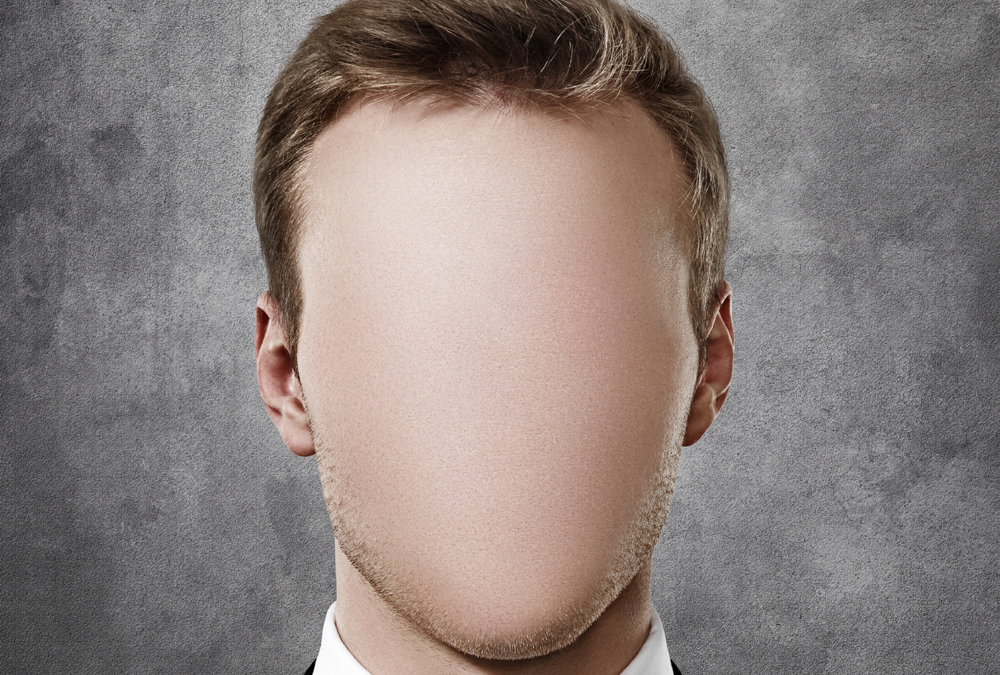
\includegraphics[width=0.35\textwidth]{Bilder/face.jpg}
\end{center}
\end{wrapfigure}
\mbox{}\\
\mbox{}\\
\mbox{}\\
\mbox{}\\
\mbox{}\\
\textbf{Aufgabenbereich}:\\
Webserver\\
Webclient\\
\textbf{Betreuer}:\\
Dip.-Ing. Manfred Steiner
\mbox{}\\
\mbox{}\\
\mbox{}\\
\mbox{}\\
\mbox{}\\

\subsection*{Florian Harrer}
\begin{wrapfigure}[15]{l}{0.5\textwidth}
\begin{center}
  \includegraphics[width=0.35\textwidth]{Bilder/Fotos/Harrer}
\end{center}
\end{wrapfigure}
\mbox{}\\
\mbox{}\\
\mbox{}\\
\mbox{}\\
\mbox{}\\
\mbox{}\\
\textbf{Aufgabenbereich}:\\
Java-Programm\\
\textbf{Betreuer}:\\
Dip.-Ing. Manfred Steiner
\mbox{}\\
\mbox{}\\
\mbox{}\\
\mbox{}\\
\mbox{}\\
\newpage

\subsection*{Dominik Pichler}
\begin{wrapfigure}[12]{l}{0.5\textwidth}
\begin{center}
  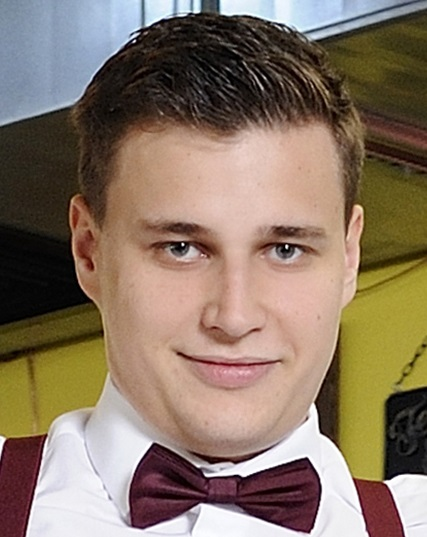
\includegraphics[width=0.35\textwidth]{Bilder/Fotos/Pichler}
\end{center}
\end{wrapfigure}
\mbox{}\\
\mbox{}\\
\mbox{}\\
\mbox{}\\
\mbox{}\\
\mbox{}\\
\textbf{Aufgabenbereich}:\\
Mechanik\\
\textbf{Betreuer}:\\
Dip.-Ing. Dr. Gerhard Pretterhofer
\mbox{}\\
\mbox{}\\
\mbox{}\\
\mbox{}\\
\mbox{}\\

\subsection*{Julian Wolf}
\begin{wrapfigure}[15]{l}{0.5\textwidth}
\begin{center}
  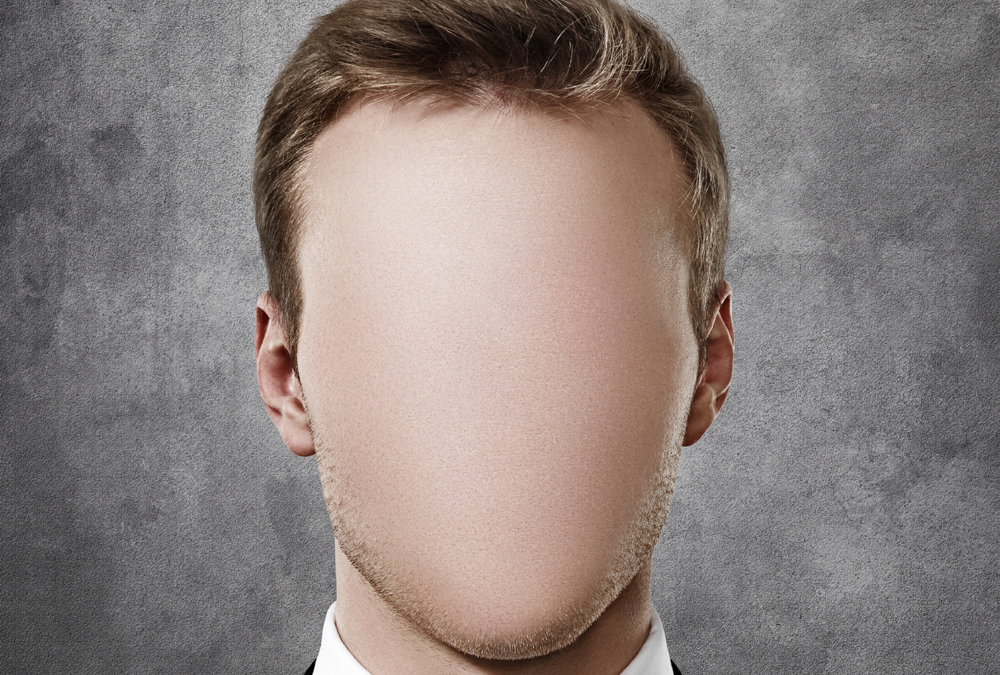
\includegraphics[width=0.35\textwidth]{Bilder/face.jpg}
\end{center}
\end{wrapfigure}
\mbox{}\\
\mbox{}\\
\mbox{}\\
\mbox{}\\
\mbox{}\\
\textbf{Aufgabenbereich}:\\
Elektrotechnik\\
Mechanik\\
\textbf{Betreuer}:\\
Otto Schuller

\tableofcontents
\mainmatter
\lohead{Florian Greistorfer}
\chapter{Webserver und Client}

\section{Begriffserklärungen}

\subsection{Server}
Ein Programm, der oder das Zugriff auf eine Resource oder einen Dienst in einem Netzwerk ermöglicht

\subsection{Client}
Ein Programm, der oder das auf einen Server zugreift

\section{Anforderungen}

\subsection{Webserver}
Auf der Katzenfütterungsanlage läuft ein Webserver, der es ermöglicht, dass der Benutzer das Gerät über das Internet erreichen kann. Hauptaufgaben des Servers sind dabei, Daten bereitzustellen, zu verabeiten und zu speichern und den Webclient zur Verfügung zu stellen.

\subsection{Client}
Der Client soll dem Benutzer ermöglichen, die Katzenfütterungsanlage über einen Webbrowser zu steuern. Ein Benutzername und ein Passwort sind erforderlich, damit man das Gerät bedienen kann. Das Design soll eindeutig und übersichtlich gehalten sein. Auf der Startseite sollen die eingestellten Fütterungszeiten zu sehen sein und eine allgemeine Übersicht. Über eine Navigationsleiste sollen die weiteren Seiten erreichbar sein:

\begin{itemize}
\item[•]Fütterrungszeiten
\item[•]Positionsinfo
\item[•]Geräteinfo
\item[•]Update
\end{itemize}

\section{Voruntersuchung}

\subsection{HTTP/HTTPS}
Das \ac{HTTP} ist der Kommunikationsstandart auf dem das Internet basiert. Eine HTTP Session wird über eine Anfrage über das \ac{TCP} an einen Server auf den Port 80 initiiert. Der Server, der auf diesem Port auf eine Anfrage wartet sendet eine Statusmeldung wie z.B. \inlinecode{bash}{HTTP/1.1 200 OK} und eine eigene Nachricht zurück. Diese Nachricht ist meist die angeforderte Resource oder eine Fehlermeldung. \ac{HTTPS} ist die Verschlüsselte Version von \ac{HTTP}. Die meist gebrauchten Anfragen sind:

\begin{itemize}
\item[•] \textbf{GET}: Fordert eine Representation der Resource an. Ein GET Request darf nur Daten abfragen und darf keinen anderen Einfluss haben.
\item[•] \textbf{PUT}: Fordert das speicher der Daten, die sich im Request-Body befinden, an. Wenn bereits eine Resource an der angegebenen \ac{URI} existiert, so wird diese geupdatet, sonst wir die Resource erstellt.
\item[•] \textbf{POST}: Fordert das speichern der Daten, die sich im Request-Body befinden, unter der angegebenen \ac{URI} an. 
\item[•] \textbf{DELETE}: Fordert das Löschen der Resource unter der angegebenen \ac{URI} an.
\end{itemize}

\subsection{JavaScript}
JavaScript ist die Sprache des Internets. Jeder herkömmliche Browser ist in der Lage, JavaScript auszuführen. Mit JavaScript ist es möglich, das Aussehen einer Webseite während der Laufzeit zu ändern, Dinge zu entfernen, hinzufügen und animieren. JavaScript ist eine objektorientierte Sprache. Es hebt sich von anderen Sprachen vorallem dadurch ab, dass die Datentypen von Variable nicht fix sind. Das bedeutet, wenn eine Variable den Datentyp \textit{number} hat und es wird ein String angehängt, verändert sich der Datentyp automatisch auf \textit{string}.

\subsection{Node.js}
Node.js ist eine Laufzeitumgebung, die es ermöglicht, dass Javascript direkt auf einem Rechner ausgeführt werden kann. Node.js kommt mit dem \ac{npm}. Mithilfe diesem Tools ist es möglich, Module zu installieren, updaten, löschen und veröffentlichen. Diese Module werden im Ordner \textit{/node\_modules} installiert und in der Datei \textit{package.json} unter \textit{dependencies}, oder mit der option \inlinecode{bash}{--save-dev} unter \textit{dev-dependencies} eingetragen. Ein neues Projekt erstellt man mit \inlinecode{bash}{npm init}. Dieses Tool erstellt die Datei \textit{package.json}, in der alle Abhängigkeiten und Informationen über das Projekt stehen. Wenn man ein Projekt kopiert, braucht man den \textit{/node\_modules} Ordner nicht mit kopieren. Man muss nur im Zielordner einmal \inlinecode{bash}{npm install} aufrufen.

\subsection{TypeScript}
TypeScript ist eine, von Microsoft entwickelte, Weiterentwicklung von JavaScript. Das bedeutet, jeder gültige JavaScript Code ist auch ein gültiger TypeScript Code. TypeScript wird vom TypeScript Compiler in sauberes JavaScript übersetzt. TypeScript ist sehr gut für größere Anwendungen geeignet. Typescript hat strenge Datentypen, Klassen und Vererbung. Die Datentypen von TypeScript sind:

\begin{itemize}
\item[•] \textbf{String}: eine Unicode codierte Zeichenkette
\item[•] \textbf{Number}: eine vorzeichenbehaftete Gleitkommazahl, kann auch hexadezimal, octal oder binär sein
\item[•] \textbf{Boolean}: true oder false
\item[•] \textbf{Array}: eine Liste von Elementen des gleichen Datentyps
\item[•] \textbf{Tuple}: eine Liste von Elementen unterschiedlichen Datentyps deren Anzahl bekannt ist
\item[•] \textbf{Enum}: eine Möglichkeit, numerischen Werten Namen zu geben
\item[•] \textbf{Any}: Datentyp unbekannt, wird behandelt wie in JavaScript
\item[•] \textbf{Void}: kein Datentyp, meist Rückgabewert bei Funktionen
\item[•] \textbf{Null}: leerer Wert, kann allen anderen zugewiesen werden
\item[•] \textbf{Undefined}: kein Wert, kann allen anderen zugewiesen werden
\item[•] \textbf{Never}: wenn ein Wert niemals auftreten kann z.B. eine Funktion die immer einen Fehler produziert
\end{itemize}

Damit JavaScript Module von TypeScript verwendet werden können, benötigen sie sogenannte Type Annotations. Diese können bei den meisten bekannteren Modulen über den \ac{npm} installiert werden. Diese Pakete haben den Namenspräfix \textit{@types/}, das bedeutet, dass zum Beispiel die Type Annotations des Express Moduls über \inlinecode{bash}{npm install --save-dev @types/express} installiert werden können. Sollten keine Type Annotations für ein Modul vorhanden sein, muss man diese selbst erstellen.

\subsection{express}
Express ist ein Javascript Modul, dass auf dem Node.js Modul \textit{http} bzw \textit{https} aufbaut. In diesen Modulen ist bereits alles enthalten, dass benötigt wird, um einen Webserver zu programmieren. Express nimmt uns die meiste Arbeit ab und bietet viele weitere Möglichkeiten.

\subsection{JSON}
\ac{JSON} ist die Textrepresentation eines JavaScript Objekts. Die möglichen Datentypen sind:

\begin{itemize}
\item[•] \textbf{string}: 0 oder mehrere unicode Zeichen innerhalb Doppelhochkommas
\item[•] \textbf{boolean}: true oder false
\item[•] \textbf{number}: Eine vorzeichenbehaftete Zahl, die auch die E Notation unterstützt z.B. 0.2E4 (=2000)
\item[•] \textbf{Array}: Eine geordnete Liste von 0 oder mehreren Werten innerhalb viereckigen Klammern, Elemente sind getrennt durch Kommas.
\item[•] \textbf{Object}: Eine ungeordnete Sammlung von Name-Wert-Paaren, wo die Namen, die auch Keys genannt werden, Strings sind; Jeder Key sollte eindeutig sein; Innerhalb geschwungener Klammern; Paare sind durch Komma getrennt
\item[•] \textbf{null}: Ein leerer Wert
\end{itemize}

\begin{lstlisting}[style=JSON,caption=\ac{JSON} Beispiel]
{
	"Object": {	
		"string": "name",
		"number": 10E5,
		"boolean": true,
		"Array": [
			{
				"string": "wert",
				"number": 1
			},
			{
				"string": "wert",
				"number": 2
			}
		]
	}
}
\end{lstlisting}

\subsection{JSON Web Token}
\ac{JWT} ist ein JSON-basierter, offener Standart für das erstellen von Access Tokens. Mithilfe eines \ac{JWT} kann ein Client sich ausweisen. Ein \ac{JWT} wird vom Server entweder mit einem Secret oder seinem privaten Schlüssel signiert. Dadurch können Server und Client beide überprüfen, ob der Token legitim ist. Ein \ac{JWT} besteht aus drei Teilen. Dem Header, der Payload und der Signature. Im Header steht der fürs Verschlüsseln der Signatur benutzte Algorythmus z.B: \inlinecode{JSON}{\{"alg":"RS256","typ":"JWT"\}}. Im Payload stehen die Daten, die entweder den Client ausweisen oder ähnliche Information. Beispiel: \inlinecode{JSON}{\{"user": "cat", "iat": 1520875121, "exp": 1520911121\}} \textit{iat} bedeutet \textit{issued at} und sagt aus, wann der Token generiert wurde. In der Signature steht der Key, der unsignierte Token, das ist der Header und die Payload Base64 codiert, und die Signatur. Alle drei Teile werden Base64 codiert und mittels Punkt voneinander getrennt.

\subsection{MongoDB}
MongoDB ist eine schemenlose Datenbank. Schemenlos bedeutet, dass die Datenbank, im vergleich zu schemenbehafteten Datenbanken, keine klare Strukturierung benötigt. Einer schemenlosen Datenbank kann man einfach Daten geben und wieder abfragen. Eine schemenbehaftete Datenbank ist in Zeilen und Spalten unterteilt. Diese müssen vorher feststehen. Da Raspian, das Betriebssystem vom Raspberry Pi, nur 32 Bit ist und MongoDB ab Version 3 nur mehr in 64 Bit erhältlich ist, mussten wir auf eine ältere Version wechseln. Die Verbindung der MongoDB Datenbank erfolgt über einen Driver. Der Driver muss mit der Datenbankversion übereinstimmen. MongoDB ist ein \ac{DBS}, das bedeutet, ein Server läuft auf dem Port 27017, über den alle Datenbanken im System erreichbar sind z.B. die Datenbank \textit{fuettr} ist über \inlinecode{bash}{localhost:27017/fuettr} erreichbar. Eine Gruppe von Daten nennt man Collection. Zugriff auf die Datenbank erfolgt serverseitig wie folgt:

\begin{lstlisting}[caption=Verbinden mit dem \ac{DBS},style=TS]
const dbServer = await mongodb.MongoClient.connect(url);
\end{lstlisting}

\begin{lstlisting}[caption=Auswählen der Datenbank,style=TS]
const dbFuettr = await dbServer.db('fuettr');
\end{lstlisting}

\begin{lstlisting}[caption=Auswählen der Collection,style=TS]
const collTimes = await dbFuettr.collection('data_times');
\end{lstlisting}

\begin{lstlisting}[caption=Auslesen aller Datensätze mit einem Identifier,style=TS]
const Times = await this._times.find({ identifier: 'Times' }).toArray();
\end{lstlisting}

\begin{lstlisting}[caption=Überschreiben eines Datensatzes mit einem Identifier,style=TS]
this._times.updateOne({ identifier: 'Times' }, { $set: times });
\end{lstlisting}

\subsection{Angular 2/4}
Angular ist ein TypeScript Framework, das aus dem Javascript-Framework AngularJS weiterentwickelt wurde. Es wird von Google entwickelt. Angular ist gegliedert in Module. Die grobe Struktur wird in der Abbildung \ref{Angular Struktur} dargestellt.

\begin{figure}[H]
      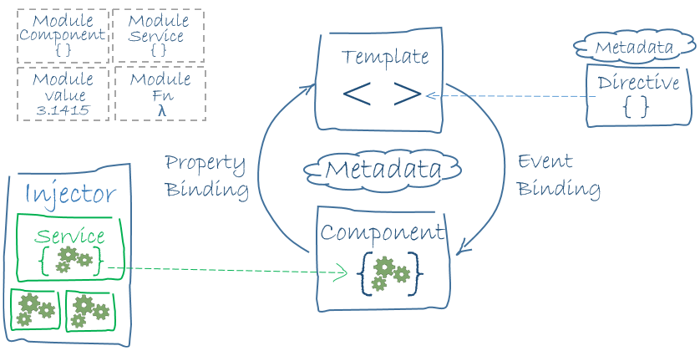
\includegraphics[width=1\textwidth]{Bilder/Greistorfer/Angular}
      \caption{Angular Struktur}
      \label{Angular Struktur}
\end{figure}

\subsubsection{Modules}
Jede Angular App ist in \textit{Module}s gegliedert. \textit{Module}s fassen meist ähnliche Funktionen zusammen. Jede App muss mindestens ein \textit{Module} enthalten. Dies heißt standartmäßig \textit{AppModule}. Ein \textit{Module} ist die größte Einheit einer Angular App.  Ein \textit{Module} kann folgende Komponenten beinhalten:

\begin{itemize}
\item[•]Services
\item[•]Andere Module
\item[•]View Classes
\begin{itemize}
\item[-]Components
\item[-]Directives
\item[-]Pipes
\end{itemize}
\end{itemize}

\subsubsection{Libraries}
Eine Angular Library ist ein Modul, das \textit{decorator} und \textit{Modules} exportiert. Diese können von \textit{Components} und \textit{Modules} importiert werden. Der Name jeder Angular library beginnt mit \textit{@angular}. Angular libraries können mit dem \ac{npm} installiert werden.

\subsubsection{Components}
Ein \textit{Component} kontrolliert einen Teil des Bildschirms, den sogenannten \textit{view}. Die Logik des \textit{Component}s wird in einer Klasse definiert. Die Klasse interagiert mit dem \textit{view} durch eine \ac{API} von Eigenschaften und Methoden.

\subsubsection{Templates}
Das Aussehen des \textit{view}s wird in einem \textit{Template} definiert. Ein \textit{Template} ist eine \ac{HTML} Datei, mit Angular's Template Syntax. Das bedeutet, dass einige Zusatzbefehle vorkommen können. Beispiele hierfür sind:

\begin{itemize}
\item[•]*ngFor
\item[•]*ngIf
\item[•]\{\{variable\}\}
\item[•](click)
\item[•][variable]
\item[•]<app-route>
\end{itemize}

\subsubsection{Data binding}
\begin{wrapfigure}{l}{0.5\textwidth}
\vspace{-30pt}
  \begin{center}
    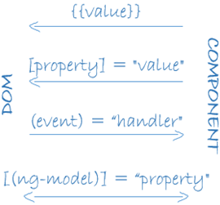
\includegraphics[width=0.5\textwidth]{Bilder/Greistorfer/databinding}
  \end{center}
  \caption{Angular Databinding}
  \label{Angular Databinding}
  \vspace{-10pt}
\end{wrapfigure}



\subsubsection{Services}

\subsection{Bootstrap}
Bootstrap ist eine CSS Bibliothek, die die Möglichkeit bietet, bereits vorgefertigte Komponenten auf unserer Website zu verwenden. An erster Stelle stehen bei Bootstrap responsive Design und Mobilgeräte. Responsive bedeutet, dass die Elemente sich an die breite des Bildschirms anpassen. Dadurch erspart man sich als nicht sehr designaffiner Programmierer viel Arbeit. Auf der offiziellen Bootstrap Website kann man außerdem verschiedene Themes auswählen. Bootstrap wurde von Twitter entwickelt und ist entweder über den \ac{npm} oder über Bootstraps eigenes \ac{CDN} erhältlich.

\section{Umsetzung}

\subsection{Projektstruktur}
\dirtree{%
.1 Webserver.
.2 server.
.3 dist.
.3 keys.
.3 node\_modules.
.3 public.
.3 src.
.4 views.
.2 ngx.
.3 dist.
.3 e2e.
.3 node\_modules.
.3 src.
.4 app.
.5 components.
.5 services.
.4 assets.
.4 environments.
.4 i18n.
}


\subsection{Client}

\subsubsection{Design}
Das Design sollte übersichtlich und einfach gestaltet werden. Der Benutzer soll auf den ersten Blick die wichtigsten Funktionen und Informationen erkennen können. \\

\begin{wrapfigure}{r}{0.7\textwidth}
\vspace{-30pt}
  \begin{center}
    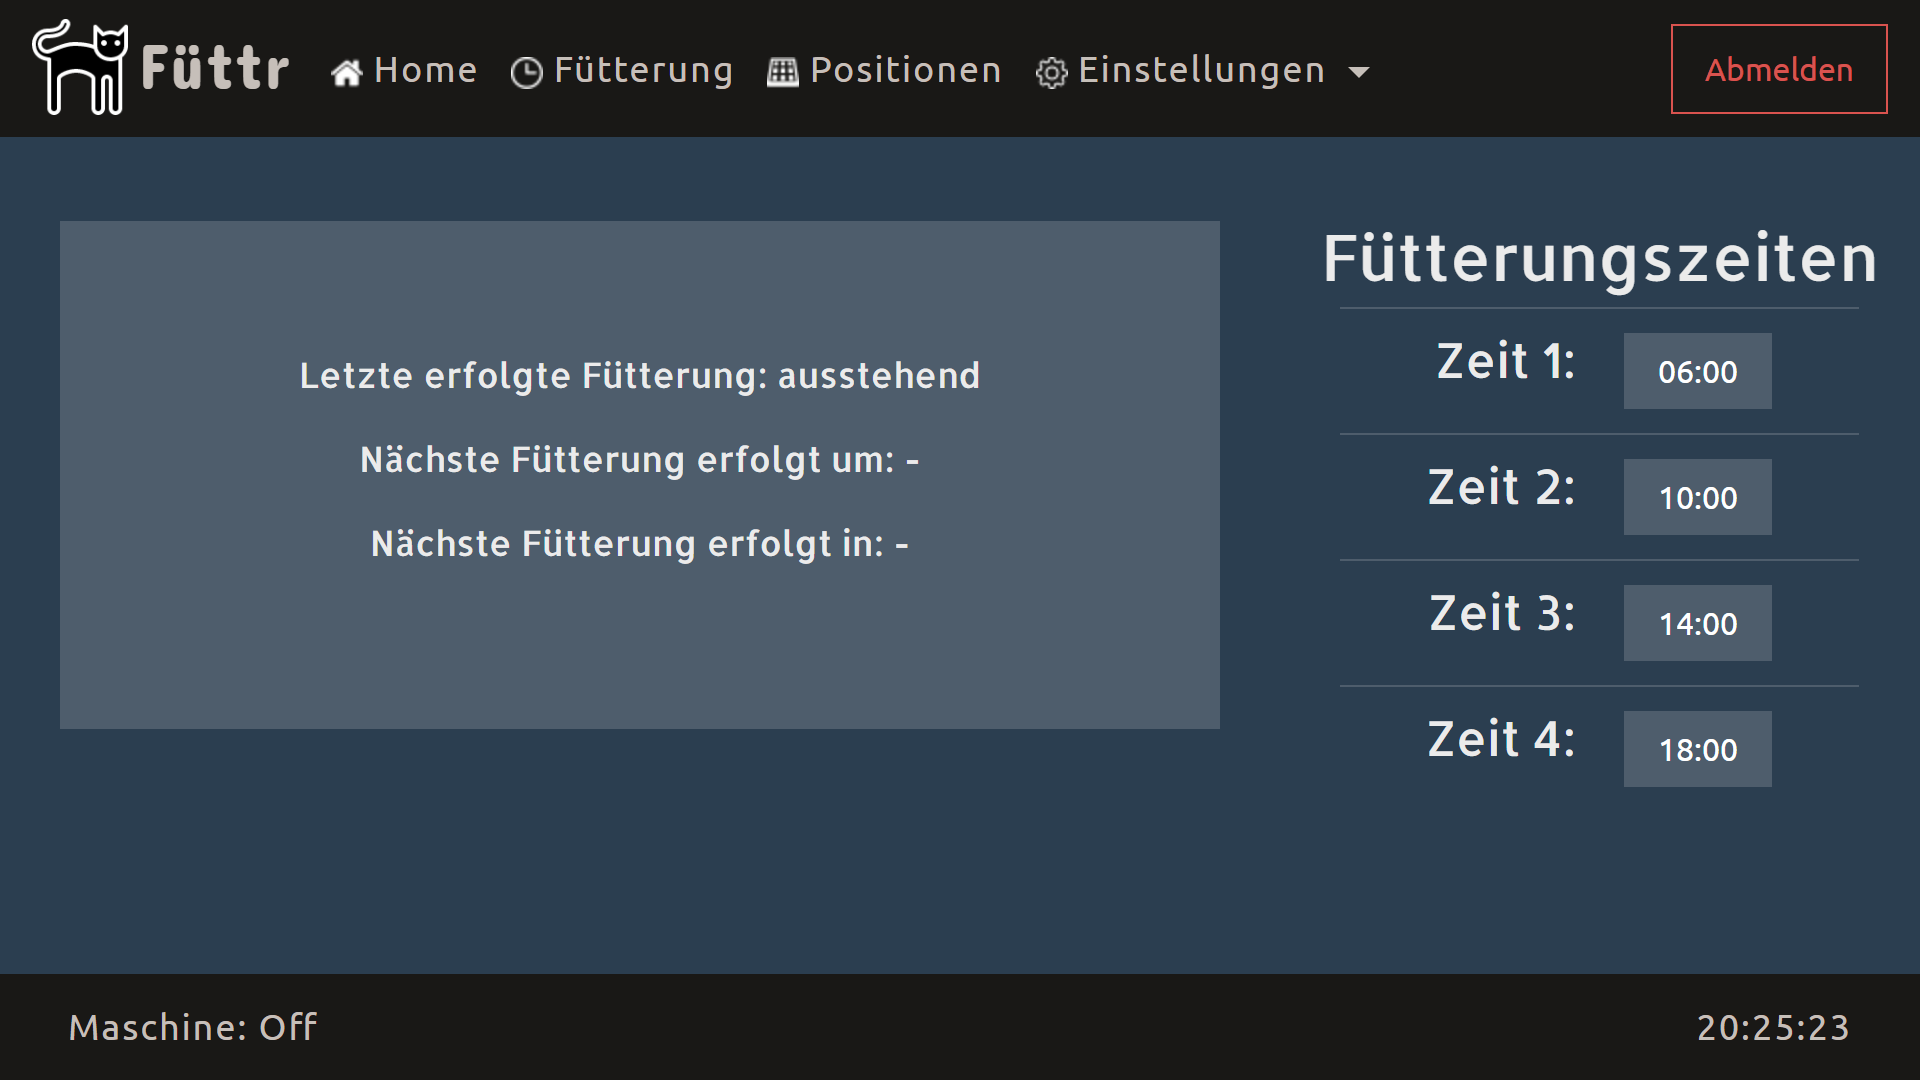
\includegraphics[width=0.7\textwidth]{Bilder/Greistorfer/Home}
  \end{center}
  \caption{Startseite}
  \label{Startseite}
  \vspace{-10pt}
\end{wrapfigure}

Auf der Starseite sind alle wichtigen Informationen übersichtlich dargestellt. Auf der linken Seite werden die Uhrzeit der letzten erfolgreichen Fütterung, die Zeit der nächsten Fütterung und die Zeit bis zur nächsten Fütterung dargestellt. Darunter werden Fehler und Warnungen, fals welche auftreten sollten, angezeigt. Da unbekannt ist, wie viele Fehler und Warnungen auftreten, werden diese in einem *ngFor aufgelistet. Auf der rechten Seite sind die aktiven Fütterungszeiten aufgelistet. \\

\begin{wrapfigure}{r}{0.7\textwidth}
\vspace{-30pt}
  \begin{center}
    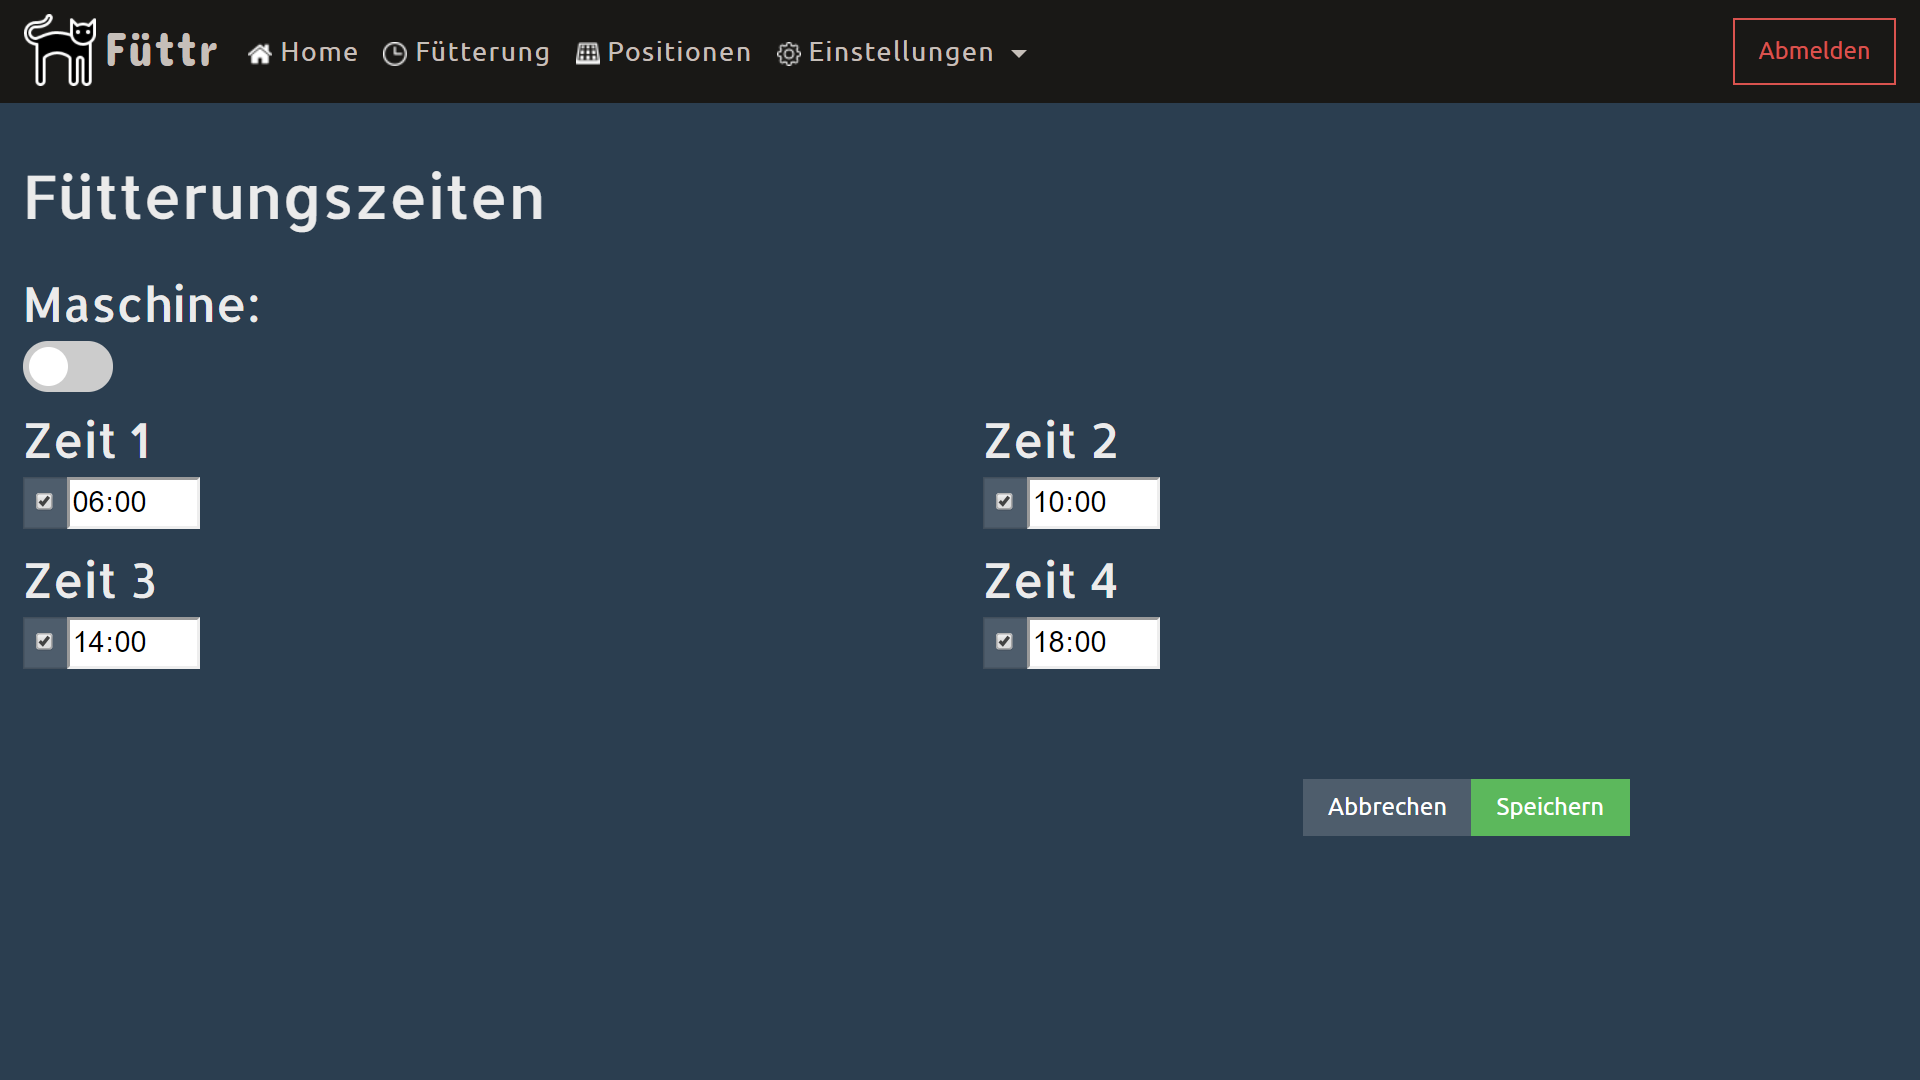
\includegraphics[width=0.7\textwidth]{Bilder/Greistorfer/Fuetterungszeiten}
  \end{center}
  \caption{Fütterungszeiten}
  \label{Fütterungszeiten}
  \vspace{-10pt}
\end{wrapfigure}

Auf der Fütterungszeiten-Seite kann der Benutzer die Katzenfütterungsanlage ein und ausschalten. Dies wurde mit einer Checkbox realisiert, die durch Styles wie ein Schalter gestaltet wurde. Darunter können die Fütterungszeiten geändert und deaktiviert werden. Siehe Abbildung \ref{Fütterungszeiten}. Der Button 'Speichern' wird deaktiviert, sobald eine Zeit ungültig eingegeben wurde, oder wenn die Zeiten nicht in aufsteigender Reihenfolge sortiert sind. \\

\begin{wrapfigure}{r}{0.7\textwidth}
\vspace{-30pt}
  \begin{center}
    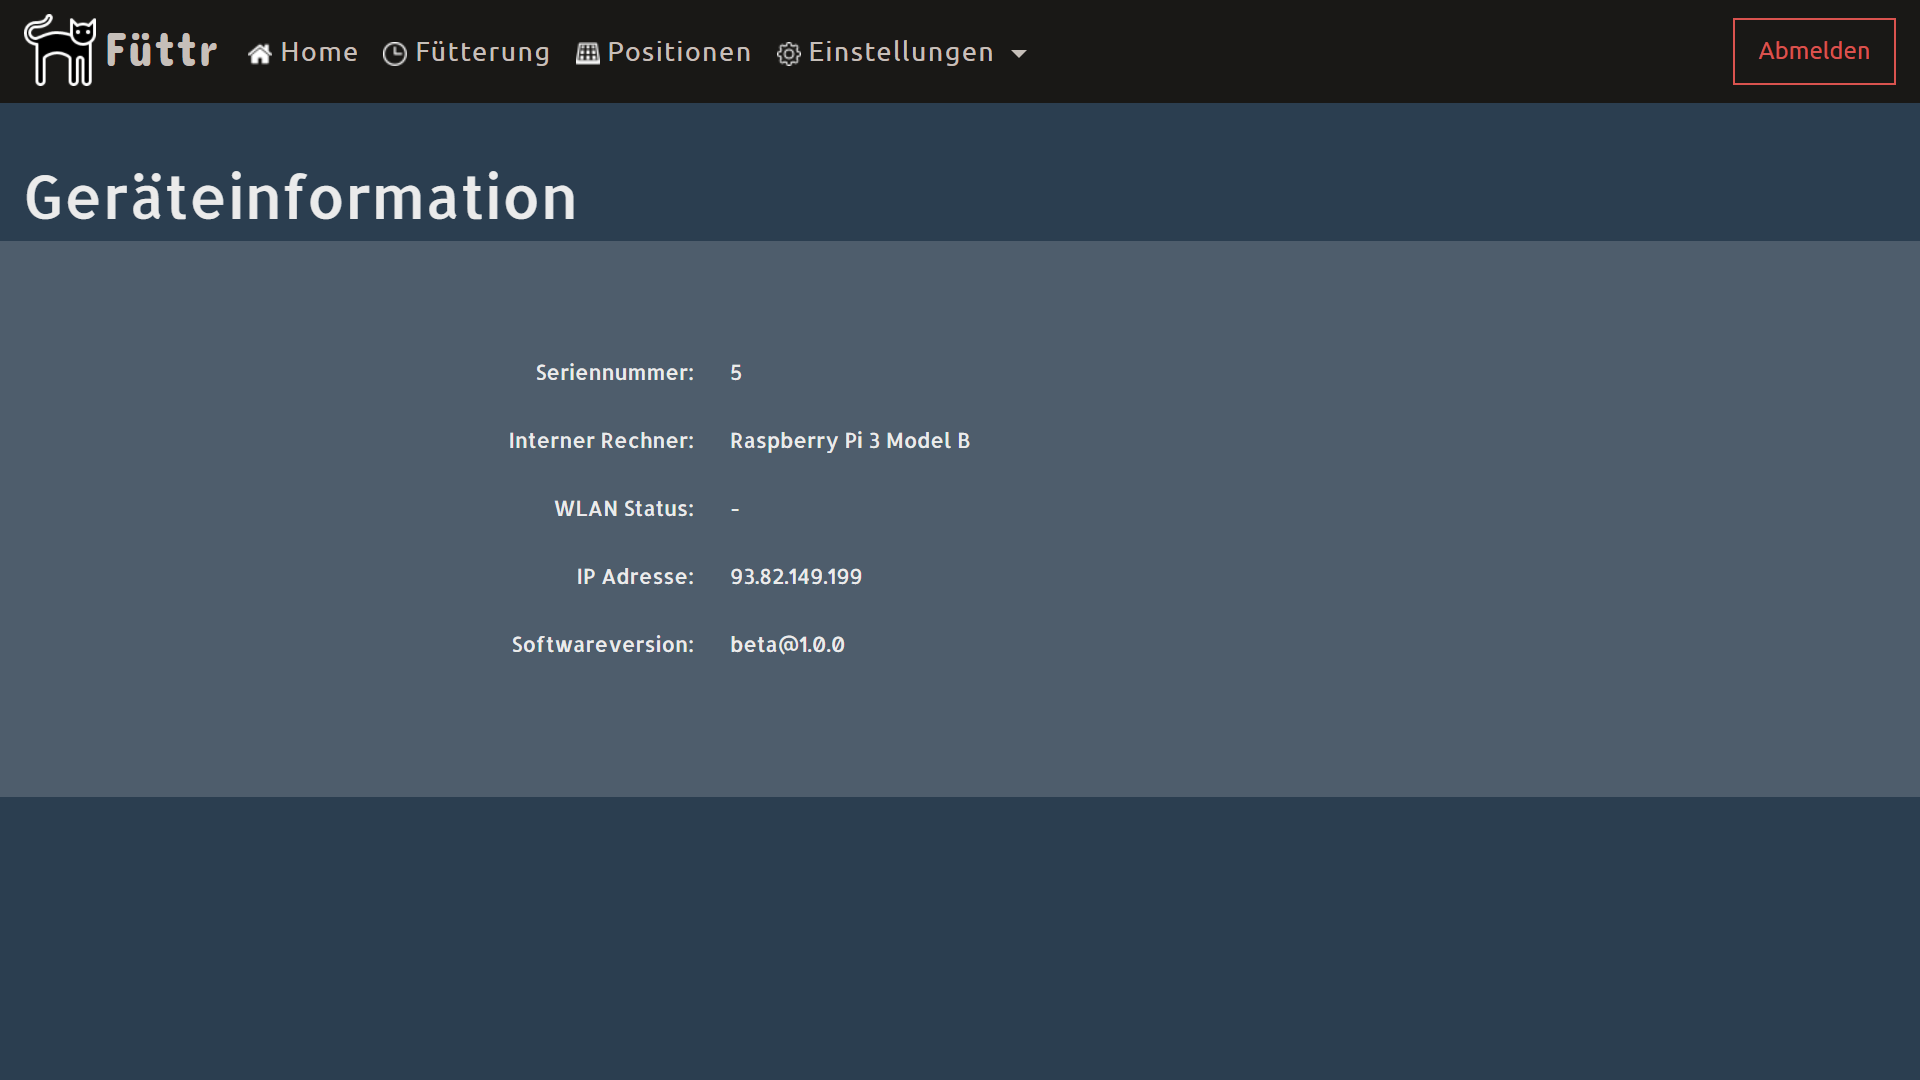
\includegraphics[width=0.7\textwidth]{Bilder/Greistorfer/Gerateinformation}
  \end{center}
  \caption{Geräteinformationen}
  \label{Geräteinformationen}
  \vspace{-50pt}
\end{wrapfigure}

Auf der Geräteinformations-Seite werden die wichtigsten Daten über das Gerät angezeigt. diese Daten sind:
\begin{itemize}
\item[•]Seriennummer
\item[•]Interner Rechner
\item[•]WLAN Status
\item[•]IP Adresse
\item[•]Softwareversion
\end{itemize}
Die Seriennummer ist eindeutig und wird von einem Server zugeteilt. Die IP-Adresse ist die aktuelle \textbf{externe} IP-Adresse. \\

\begin{wrapfigure}{r}{0.7\textwidth}
\vspace{-30pt}
  \begin{center}
    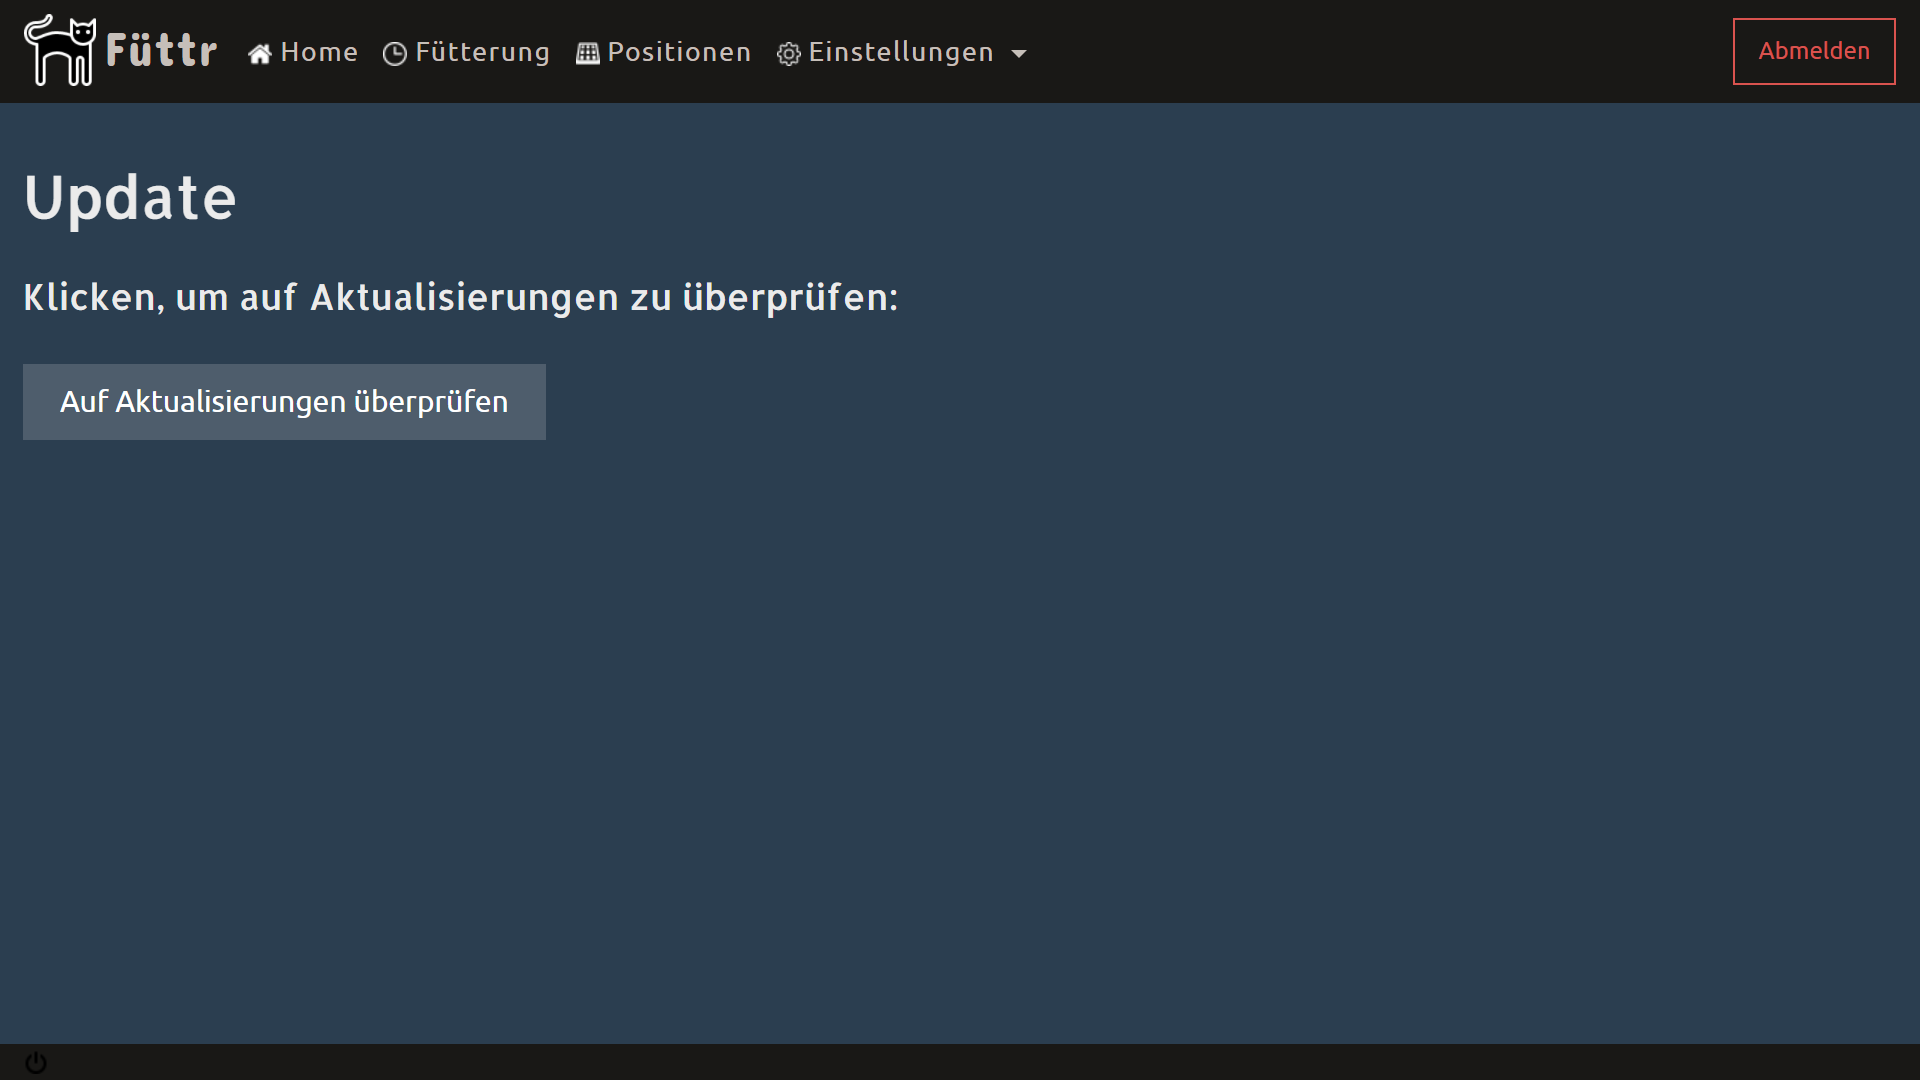
\includegraphics[width=0.7\textwidth]{Bilder/Greistorfer/Update}
  \end{center}
  \caption{Update}
  \label{Update}
  \vspace{-10pt}
\end{wrapfigure}

Auf der Update-Seite kann der Benutzer nach Updates suchen, Updates starten oder die Maschine herunterfahren. Wenn der Benutzer auf den Herunterfahren-Button klickt, der sich auf der linken Seite ganz unten befindet, wird er gewarnt, dass die Maschine nur mehr über das Aus- und wieder Einstecken des Netzteils startbar ist.\\

\subsubsection{Funktion}

\subsection{Server}

\subsubsection{Funktion}

\subsubsection{Mongodb}

\subsubsection{Kommunikation mit dem Java Programm}

\section{Zusammenfassung und Verbesserungsmöglichkeiten}
\lohead{Florian Harrer}

\chapter{Java-Programm}
\label{sec:java-programm}

\section{Anforderungen}
\subsection{Programm}
Die Hauptaufgabe des Programms ist es dem Benutzer eine Möglichkeit zum Steuern der Katzenfütterungsanlage zu Verfügung zu stellen. Weiters soll das Programm die Motoren steuern und die Sensoren in der Anlage auswerten können. Für diese Aufgabe sollen die IO-Pins am Raspberry verwendet werden.
\subsection{Design - Benutzerinterface}
Das Design der GUI-Fenster soll einfach und übersichtlich gestaltet werden. Auf der Hauptseite, also der Seite die immer zu sehen ist, sollen Informationen dargestellt werden, die dem Benutzer einen schnellen Überblick über den Zustand der Anlage geben. Alle anderen nicht direkt ersichtlichen Funktionen sollen über sinnvoll benamte Menüpunkte erreichbar sein.
Der Benutzer soll mit Hilfe eines kleinen Touchdisplays die Möglichkeit haben die Anlage zu steuern. Deswegen muss darauf geachtet werden, dass alle GUI-Fenster sinnvoll per Touch-Gesten verwenbar sind.
\subsection{Externe Steuerung}
Da die Katzenfütterungsanlage die Katze füttern soll, wenn die Familie der Katze auf Urlaub ist, sollte die Anlage auch über das Internet erreichbar sein. Dafür gibt es die Möglichkeit einen Benutzer auf der Anlage anzulegen mit welchem man anschließend über eine Webseite auf die Anlage zugreifen kann. Weiters soll das Java Programm (Server) mit der Web-Applikation (Client) kommunizieren, also Daten austauschen, können.

\newpage

\section{Voruntersuchung}
\subsection{Wieso Java und nicht C?}
Zu Beginn musste entschieden werden mit welcher Programmiersprache gearbeitet werden soll. Zur Auswahl standen Java und C.
Vorteile von C:
\begin{itemize}
\item[1] Echtzeitfähige Steuerung der Motoren und Senosren
\item[2] Hardwarenahe Programmierung für die Pins
\end{itemize}
Vorteile von Java:
\begin{itemize}
\item[1] Erstellen einer GUI ist einfacher
\item[2] Implementieren eines Servers ist einfacher
\end{itemize}

Nach dem Gegenüberstellen der Vorteile wurde Java als Programmiersprache gewählt.

\subsection{Wieso das Raspberry Pi 3 Model B?}
Schon zu Beginn der Diplomarbeit war klar, dass mit deinem Raspberry gearbeitet werden soll. Nun musste entschieden werden welches Model verwendet werden soll. Wir haben das Raspberry Pi 3 Model B aufgrund folgender technischer Daten gewählt:
\begin{itemize}
\item[1] Rechenleistung
\item[2] Anzahl der GPIO-Pins
\item[3] WLAN-Fähigkeit
\end{itemize}

\subsection{Auswahl eines Touchdisplays}
Das Display muss folgendet Anforderungen erfüllen:
\begin{itemize}
\item[1] Es muss ein Touchscreen-Display sein
\item[2] Es muss einfach an das Raspberry anschließbar sein
\item[3] Es sollte nicht zu teuer sein
\end{itemize}

Aufgrund dieser Anforderungen wurde das Touchdisplay von Raspberry gewählt.

\subsection{Wieso pi4j?}
Da Java als Programmiersprache gewählt wurde, musste eine Möglichkeit die GPIO-Pins anzusteuern gefunden werden.
Da bei der Recherche außer pi4j Java kaum etwas gefunden wurde, wurde pi4j gewählt. Weiters vorteilhaft ist, dass das Ansteuern der Pins via Code nicht sehr kopliziert ist. 

\subsection{Wieso Mongodb?}
Eine Datenbank wurde gewählt, weil es gegebüber des Speichers der Daten in eine Datei mehrere Vorteile aufweist. 
\subsubsection{Vorteil gegenüber Daten in Datei speichern}
Vorteile einer Datenbank:
\begin{itemize}
\item[1] Keine Probleme mit Pfaden
\item[2] Daten sind alle in einem Punkt gespeichert und nicht im System verteilt
\item[3] Der benötigte Code für die Datenbank macht das Programm übersichtlicher
\end{itemize}
\subsubsection{Vergleich mit anderen Datenbanken}
Vorteile von Mongodb gegenüber anderen Datenbanken (zB mySQL):
\begin{itemize}
\item[1] Mongodb ist schemenlos (Daten benötigen keine bestimmte Struktur)
\item[2] Mongodb ist kostenfrei
\end{itemize}

\subsection{Kommunikation mit der Web-Applikation}
Der Server mit dem die Web-Applikation kommunizieren kann, wird aufgrund der gewählten Programmiersprache, in Java geschrieben. Der Server wird im Hintergrund aktiv sein und auf Anfragen der Web-Applikation warten. Je nach Anfrage wird der Server Daten zurück senden oder Methoden im Programm aufrufen. Die Daten, die bei der Kommunikation ausgetauscht werden, haben den Datentyp JSON.

\newpage

\section{Umsetzung}
Bei der Umsetzung, also beim Schreiben des Programms, wurde wie folgt vorgegangen. Zuerst wurden alle GUI-Fenster per Hand grob designed. Anschließend wurden diese im Netbeans als JFrame Form erstellt. Genaueres über die GUI-Fenster folgt uner Punkt 2.3.4. Danach wurden grundlegende Funktionen die das Programm zu erfüllen hat implementiert. Weiters wurden noch: Mongodb, pi4j, der Server und der ErrorAndWarningHandler als Singleton implementiert. 
\\ \\ 
Nun folgen ausführlichere Beschreibungen über die oben angeführten Klassen.

\subsection{Mongodb}
\subsubsection{Allgemeines}
Mongodb is ein schemenlose Datenbank. Schemenlos bedeuted, dass die Daten keine besondere Formatierung brauchen um gespeichert zu werden. Zusätzlich wird jedem gespeichertem Datensatz automatisch ein einmaliger Indentifikator gegeben. Weiters ist es kostenfrei und man benötigt keine Lizenzen.
\\
Bei einer schemenbehafteten Datenbank werden die Daten in Reihen und Spalten gegliedert. Um eine solche Datenbank effizient nutzen zu können wird auch ein einmaliger Identifikator.
\\ \\ 
In Mongodb sind Zeilen Collections und Spalten Documents. 
\\ \\
Die Datenbank kann in der Konsole mit dem Befehl \textbf{mongod} gestartet werden. In unserem konkreten Fall am Raspberry startet die Datenbank beim Starten des Raspberry automatisch. Weiters kann in der Konsole mit dem Befehl \textbf{mongo}, sofern die Datenbank gestartet ist, die Mongo-Shell geöffnet werden. In der Shell können alle angelegten Datebanken verwaltet werden. Unter verwalten wird das Ändern, Hinzufügen und Löschen von Daten verstanden. Es können auch neue Datenbanken angelegt oder alte Datenbanken gelöscht werden. 
\\ Befehle:
\begin{itemize}
\item[•] \textbf{show dbs} ... zeigt alle angelegten Datenbanken an
\item[•] \textbf{show collections} ... zeigt alle collections in einer Datebank
\item[•] \textbf{use} ... verwenden einer Datenbank, falls die Datenbank noch nicht existiert wird sie neu erstellt 
\\     (Beispiel: use <Datenbankname>)
\item[•] \textbf{drop()} ... löschen einer Datenbank
\\     (Beispiel: <Datenbankname>.drop() )
\item[•] \textbf{find()} ... suchen nach bestimmten Daten 
\\     (Beispiel: db.data.find() )
\item[•] \textbf{count()} ... zählt die Dokumente in einer Collection
\\     (Beispiel: db.<Collectionname>.count() )
\item[•] \textbf{insert()} ... hinzufügen eines Dokumentes
\\     (Beispiel: db.data.insert(\{"time1":"13:30"\})
\item[•] \textbf{updateOne()} ... updaten von Daten
\\     (Beispiel: db.data.updateOne(<DokumentID>, <Daten>) )
\item[•] \textbf{deleteOne()} ... löschen eins Dokumentes
\\     (Beispiel: db.data.deleteOne(<DokumentID>) )

\end{itemize}

\subsubsection{Datenbankmanagementsystem DBS}
Ein Datenbankmanagementsystem verwaltet eine oder mehrere Datenbanken. Mehrer Datenbanken werden dabei benötigt, wenn mehrere Anwenugen oder Programme jeweils eine eigene Datenbank brauchen. Ein Beispiel für ein DBS ist Mongodb.

\subsubsection{Singleton}
Der Datenbankzugriff wurde in einem Singleton implementiert. Dadurch wird nur ein Objekt der Datenbank erzeugt. Das bedeutet, dass nur von dieser Klasse aus auf die Datenbank zugegriffen wird und nur eine Verbindung geöffnet wird.
\\ Ein weiterer Vorteil davon ist, dass wenn einmal eine andere Datenbank verwendet werden sollte, nur diese eine Klasse geändert werden muss, weil nur in dieser Klasse der Code für die spezifische Datenbank enthalten ist.

\subsubsection{Code Beispiele}
Da am Raspberry die neueste Version von Mongodb nicht funktioniert, wird die Version 2.14.2 verwendet. Weitere Details zu diesem Thema sind unter Punkt 2.4.1 zu finden.
\\ Aus diesem Grund sind auch die Methoden, die als Beispiele angeführt sind, von der älteren Version. 
\\ \\ 
Als erstes muss eine Verbindung mit der Datenbank aufgebaut werden. Falls die Datenbank noch nicht existiert wird sie automatisch erstellt.
Dies ist in Java mit folgenden Methoden möglich:
\begin{lstlisting}[style=JavaStyle, caption=Mit Mongodb verbinden]
	MongoClient mongodb = new MongoClient();
	DB database = mongodb.getDB("<Datenbankname>");
\end{lstlisting}

Danach muss die Collection, in der gearbeitet werden soll, ausgewählt werden. Falls die Collection noch nicht existiert wird sie automatisch erstellt. Das ist mit der folgenden Methode möglich:
\begin{lstlisting}[style=JavaStyle, caption=Collection auswählen]
	DBCollection coll = database.getCollection("<Collectionname>");
\end{lstlisting}
Anschließend kann mit der Datenbank gearbeitet werden. 
\begin{itemize}
\item[•] Die Dokumente in einer Collection zähle1n:
\begin{lstlisting}[style=JavaStyle, caption=Anzahl der Collections zählen]
	<Collectionname>.count();
\end{lstlisting}
\item[•] Ein Dokument aus der Datenbank lesen:
\begin{lstlisting}[style=JavaStyle, caption=Nach Dokument suchen]
	DBObject document = <Collectionname>.find(<Identifikator>).next();
\end{lstlisting}
\item[•] Ein Dokument zu einer Collection hinzufügen:
\begin{lstlisting}[style=JavaStyle, caption=Ein Dokument hinzufügen]
	<Collectionname>.insert(document);
\end{lstlisting}	
\item[•] Ein Dokument in einer Collection updaten:
\begin{lstlisting}[style=JavaStyle, caption=Ein Dokument updaten]
	<Collectionname>.update(<Identifikator>, document);
\end{lstlisting}
\end{itemize}

Bevor das Java Programm beendet wird sollte die Verbindung zur Datenbank wie folgt getrennt werden: 
\begin{lstlisting}[style=JavaStyle, caption=Verbindung zur Datenbank trennen]
	mongodb.close();
\end{lstlisting}

Ein konkretes Beispiel des Codes aus dem Programm für die Katzenfütterungsanlage sieht so aus:
\begin{lstlisting}[style=JavaStyle, caption=Konkretes Beispiel: Dokument suchen]
	DBObject document = collUser.find(
			new BasicDBObject("identifier", "User")).next();
\end{lstlisting}
Diese Zeile Code sucht in der Collection \textbf{collUser} nach dem Dokument mit dem Identifikator \textbf{new BasicDBObject(\grqq{}identifier\grqq{}, \grqq{}User\grqq{})}. Das gefundene Dokument wird dann der Varibale \textbf{document} zugewiesen. 


\subsection{pi4j} \label{subsec:pi4j}
\subsubsection{Allgemeines}
Pi4j ist eine freie Software, welche Bibliotheken zur Verfügung stellt, mit denen es möglich ist, von einem Java Programm, auf die IO-Pins eines Raspberrys zuzugreifen. Dabei kann ein GPIO-Pin als In- oder Ouput definiert werden. Wenn ein Pin als Output definiert wird, kann er den State High (+5V) oder Low (0V) haben. Mit einem Input Pin, können Signale gemessen werden. Das Ergebnis der Messung ist wieder High oder Low. Weiters ist es auch möglich einem Pin einen Listener zuzuweißen. Dieser Listener wartet bis auf diesem Pin ein Event auftritt und führt dann zum Beispiel eine Methode aus. 
\\ \\
Pi4j stellt eine Verbindung von der JVM (Java Virtuaul Machine) zu dem nativen System des Raspberys her. Dadurch wird es möglich von dem Programm auf die Pins zuzugreifen. Die folgende Grafik zeigt welche Bibliotheken dazu verwendetwerden.

\begin{wrapfigure}{l}{0.5\textwidth}
\vspace{-35pt}
  \begin{center}
    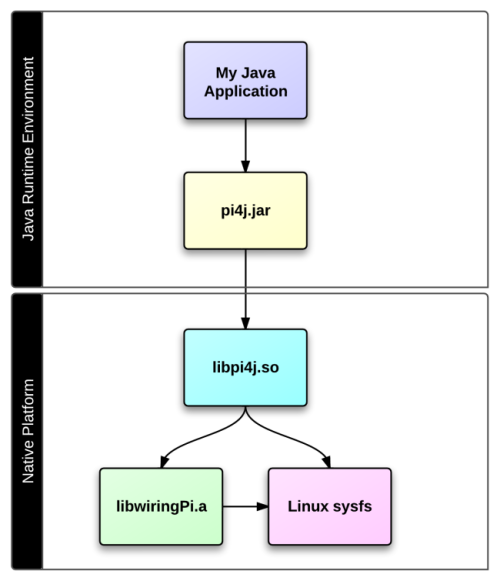
\includegraphics[width=0.45\textwidth]{Bilder/pi4j/dependencies}
  \end{center}
  \caption{Abhängigkeiten}
  \label{Magazin Vorne}
  \vspace{-170pt}
\end{wrapfigure}

Pi4j stellt eine Verbindung von der JVM (Java Virtuaul Machine) zu dem nativen System des Raspberys her. Dadurch wird es möglich von dem Programm auf die Pins zuzugreifen. Die folgende Grafik zeigt welche Bibliotheken dazu verwendetwerden.

\newpage

\subsubsection{Pin Numbering Sheme}

\begin{wrapfigure}{l}{0.5\textwidth}
\vspace{-40pt}
  \begin{center}
    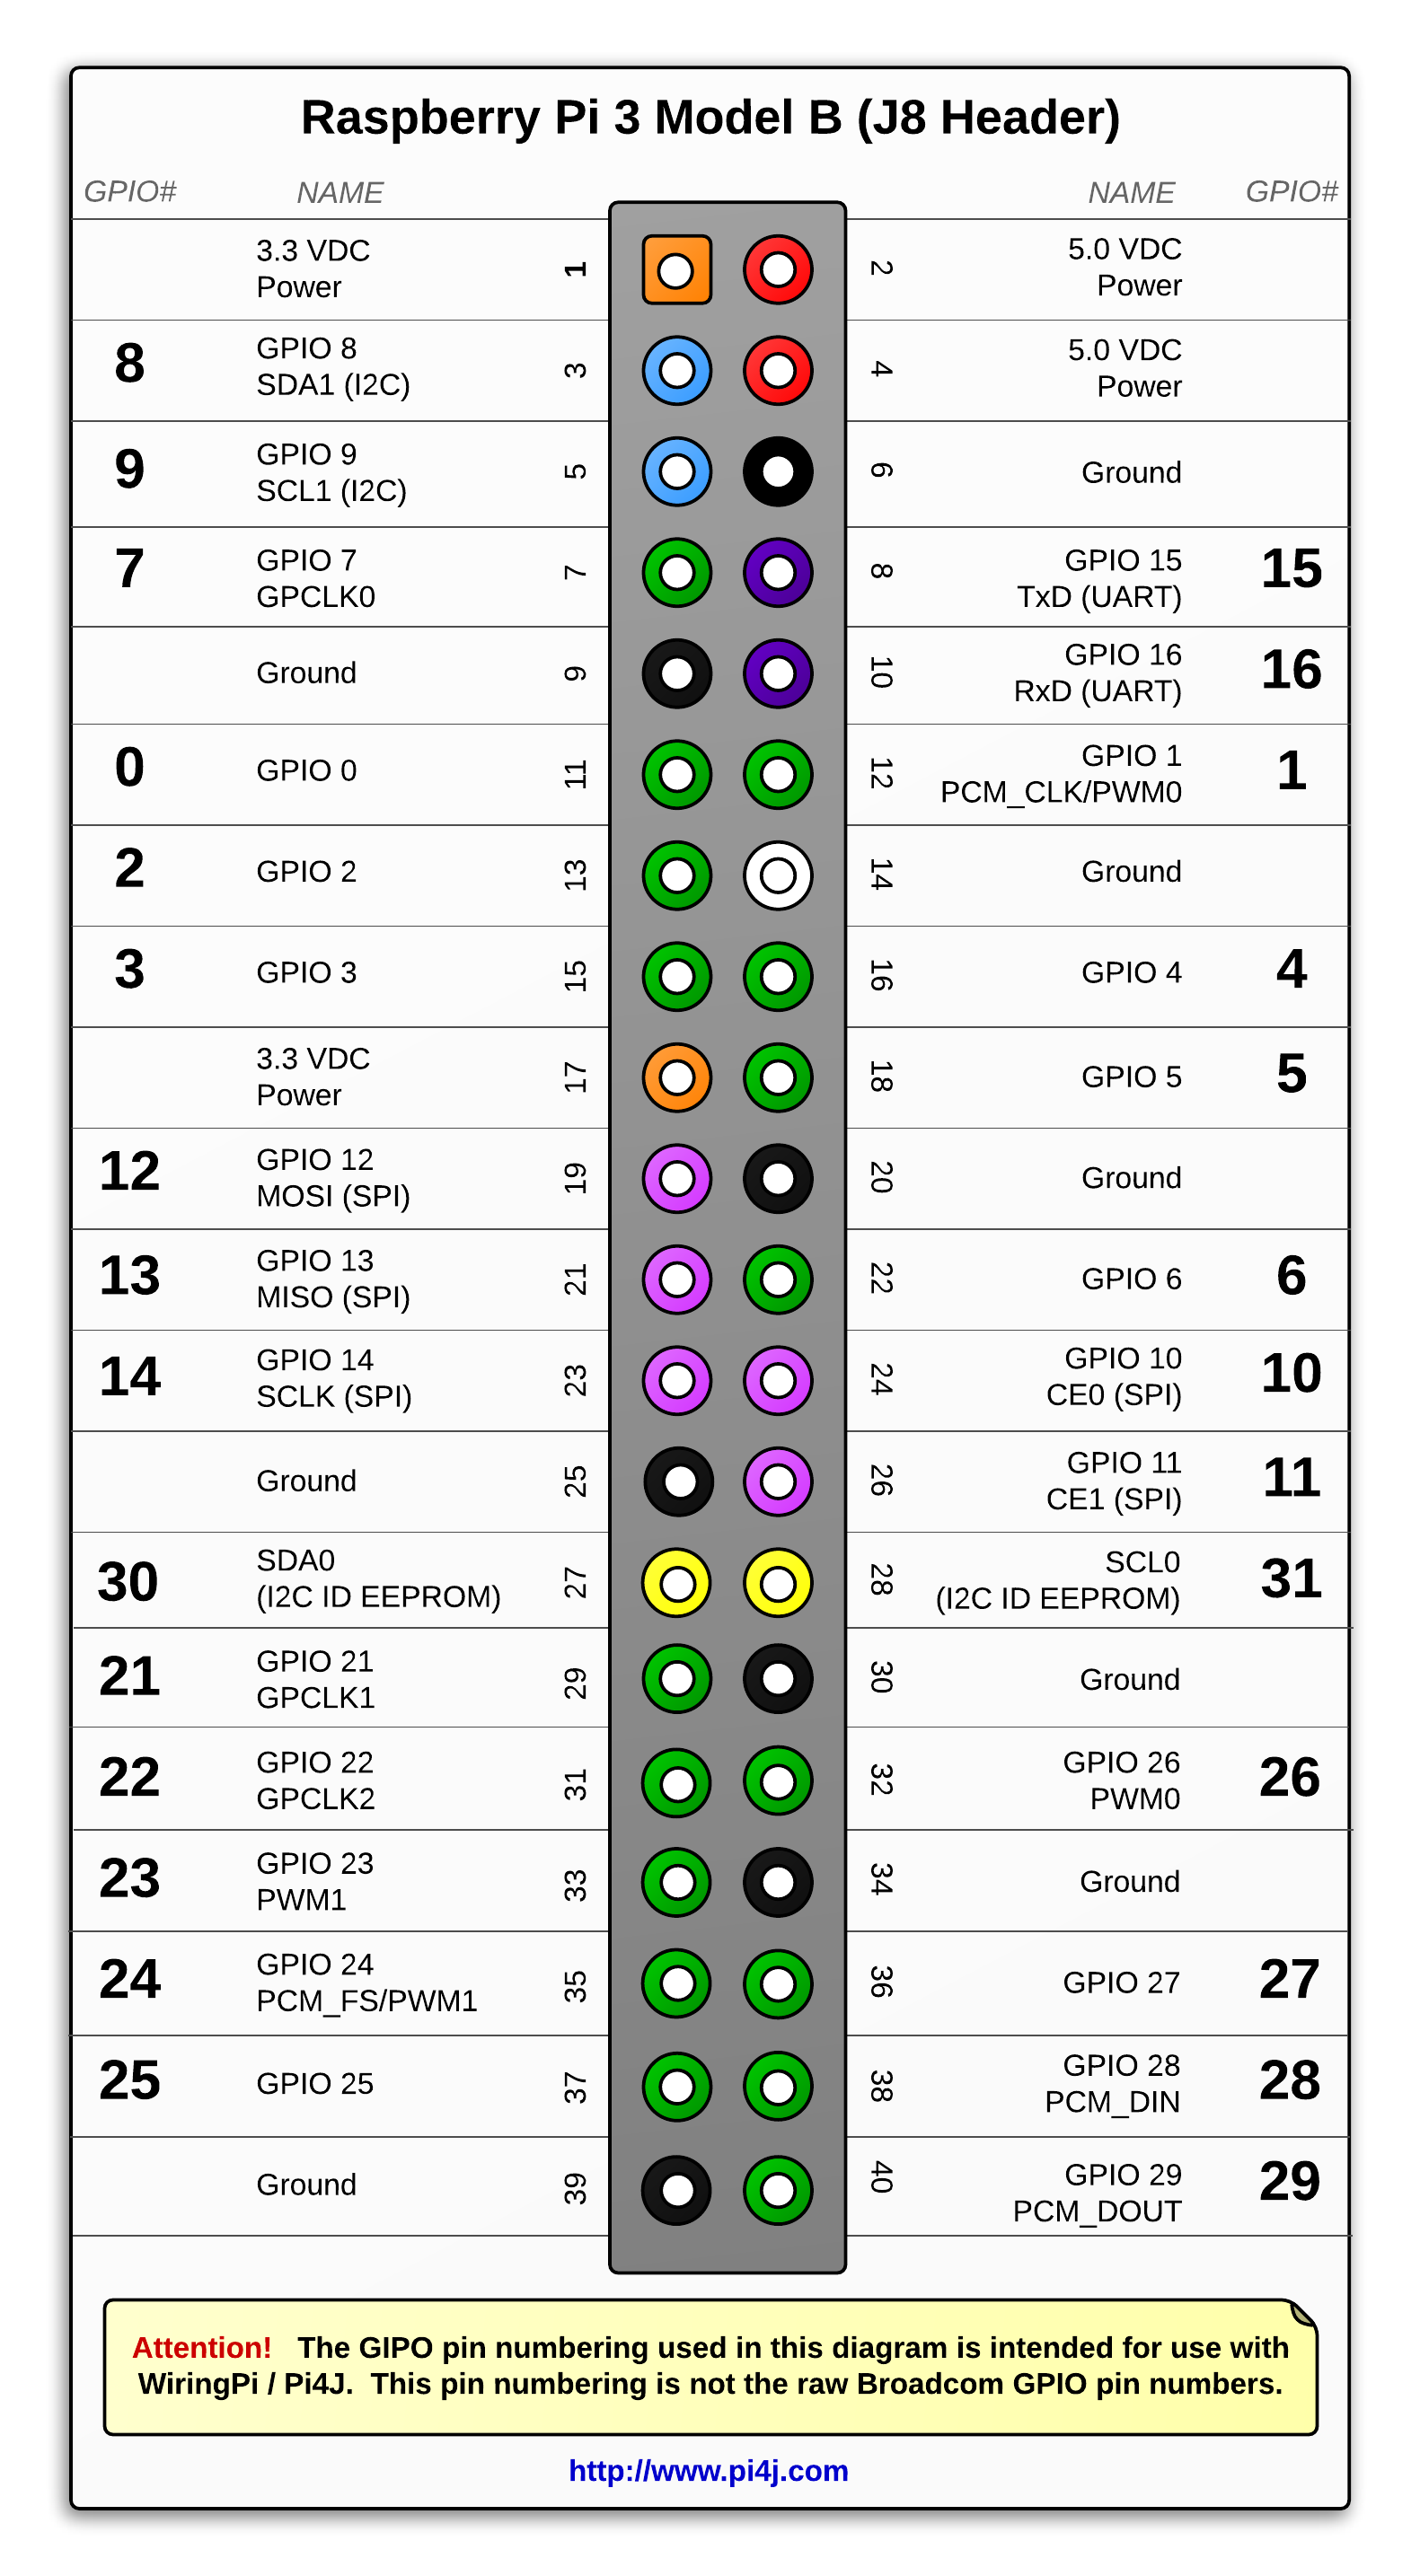
\includegraphics[width=0.50\textwidth]{Bilder/pi4j/PinNumberingSheme}
  \end{center}
  \caption{Pin Numbering Sheme}
  \label{Magazin Vorne}
  \vspace{-320pt}
\end{wrapfigure}

Am Raspberry haben einige Pins schon fest zugewiesene Funktionen, aber bei den GPIO-Pins kann der Programmierer selbst entscheiden, was der Pin sein soll.
\\ \\
In der Grafik ist zu sehen wie die Pins bei einem Raspberry Pi 3 Model B belegt sind.

\vspace{300pt}

\subsubsection{Gewählte Pin Belegung}
Zum Ansteuern der Motoren und Auswerten der Sensoren wurden nur GPIO-Pins verwendet. Die Motoren in der Anlage werden über jeweils eine H-Brücke angesteuert. Das bedeutet, dass jeder der zwei Motoren jeweils mit vier Transitoren angesteuert wird. Jeder Transitor wird von einem eigenen Pin angesteuert. Für die Sensoren wird jeweils ein Pin zum Auswerten benötigt. In Summe werden zehn GPIO-Pins benötigt. 

\newpage

Diese GPIO-Pins werden, wie folgenden Tabelle 2.1 veranschaulicht, verwendet:

\begin{table}[htb]
\centering
\begin{tabular}{|l|l|}
\hline
\textbf{Pin} & \textbf{Verwendungszweck}          \\ \hline
GPIO\_00     & Sensor Schüsselplatte              \\ \hline
GPIO\_01     & Sensor Förderband (Futtersackerl)  \\ \hline
GPIO\_02     & Motor Schüsselplatte: Transistor 1 \\ \hline
GPIO\_03     & Motor Schüsselplatte: Transistor 2 \\ \hline
GPIO\_04     & Motor Schüsselplatte: Transistor 3 \\ \hline
GPIO\_05     & Motor Schüsselplatte: Transistor 4 \\ \hline
GPIO\_06     & Motor Förderband: Transistor 1     \\ \hline
GPIO\_10     & Motor Förderband: Transistor 2     \\ \hline
GPIO\_08     & Motor Förderband: Transistor 3     \\ \hline
GPIO\_09     & Motor Förderband: Transistor 4     \\ \hline
\end{tabular}
\caption{Belegung der GPIO-Pins}
\label{Pinbelegung}
\end{table}

Wenn einer der beiden Sensoren betätigt wird, liefert dieser das Signal High (+5V). Wenn der Sensor nicht betätigt ist liefert dieser Low (0V). 
\\ Um einen Motor einzuschalten müssen jeweils zwei diagonal zueinander liegende Transitoren aktiviert werden. Der Motor dreht sich im Uhrzeigersinn, GPIO-Pins von Transistor 1 und Transistor 4 High sind. Gleichzeitig muss sicher gestellt werden, dass die GPIO-Pins der Transistoren 2 und 3 Low sind. Wenn das nicht sichergestellt ist kann es zu einem Kurzschluss zwischen der Spannungsversorgung und GND kommen. Um den Motor gegen den Uhrzeigersinn zu drehen müssen die GPIO-Pins der Transistoren 2 und 3 auf High sein. 

\subsubsection{Singleton}
Die benötigten Methoden von pi4j wurden in einem Singleton implementiert. Es musste ein Singleton verwendet werden, weil der benötigte Controller für die Pins nur einmal erzeugt werden kann. Wenn der Controller trotzdem öfters erzeugt wird, wird  ein Error geworfen. Der Singleton wird nun dazu verwendet, dass auf die Pins von unterschiedlichen Klassen zugegriffen werden kann. Der Zugriff von mehreren Klassen ist ohne einen Singleton programmiertechnisch nicht lösbar.

\subsubsection{Code Beispiele}
Um mit den GPIO-Pins arbeiten zu können muss zu Beginn ein Controller erstellt werden. Dies ist wie folgt möglich:
\begin{lstlisting}[style=JavaStyle, caption=GPIO-Controller erstellen]
	GpioController controller = GpioFactory.getInstance();
\end{lstlisting}
Wenn der Controller erstellt ist kann auf die Pins, mit denen gearbeitet werden soll, zugegriffen werden. Bei einem Pin kann auch eine \textbf{ShutDownOption} angeben werden. Diese gibt an in welchen Zustand der Pin vor dem Herunterfahren gesetzt wird. Dieser Zugriff erfolgt wie folgt: 
\begin{itemize}
\item[•] Zugreigen auf einen Pin als digitalen Input-Pin:
\begin{lstlisting}[style=JavaStyle, caption=Zugriff auf einen Pin als Inpput]
	GpioPinDigitalInput pin = controller.provisionDigitalInputPin(
		RaspiPin.GPIO_00, PinPullResistance.PULL_DOWN);
	pin.setShutdownOptions(true);
\end{lstlisting}
\item[•] Zugreigen auf einen Pin als digitalen Output-Pin:
\begin{lstlisting}[style=JavaStyle, caption=Zugriff auf einen Pin als Output]
	GpioPinDigitalOutput pin = controller.provisionDigitalOutputPin(
		RaspiPin.GPIO_02, PinState.LOW);
	pin.setShutdownOptions(true, PinState.LOW);
\end{lstlisting}
\end{itemize}
Wenn das erledigt ist kann mit dem Pin gearbeitet werden. Dies kann wie in den folgenden Beispielen erfolgen:
\begin{itemize}
\item[•] Zustand eines Input-Pins auswerten: 
\begin{lstlisting}[style=JavaStyle, caption=Pinzustand abfragen]
	pin.getState()
\end{lstlisting}
Diese Methode liefert den Zustand des Pins zurück. Dieser kann High oder Low sein.
\item[•] Zustand eines Output-Pins setzen:
\begin{lstlisting}[style=JavaStyle, caption=Pinzustand verändern]
	pin.low();	
	pin.high();
\end{lstlisting}
Mit \textbf{pin.low()} kann der Zustand eines Pins auf Low (0V) und mit \textbf{pin.high()} auf High (+5V) gesetzt werden. 
\end{itemize}

Vor dem Beenden des Java Programmes sollte der Controller wie folgt heruntergefahren werden:
\begin{lstlisting}[style=JavaStyle, caption=Controller herunterfahren]
	controller.shutdown();
\end{lstlisting}

\newpage

\subsection{Server-Client-Kommunikation}
\subsubsection{Server}
Der Server wird beim Starten des Java Programmes in einem eigenen Thread gestartet. In diesem Thread wartet der Server bis ein Client versucht Kontakt mit ihm aufzunehmen. Wenn die Verbindung akzeptiert wird, wird ein neuer Thread geöffnet in dem die Kommunikation mit diesem Client abläuft. Sobald die Kommunikation beendet ist wird der Thread wieder geschlossen. 
\\ Der Server wurde auch als Singleton implementiert damit von mehreren Klassen ausgehend auf ihn zugegriffen werden kann.

\subsubsection{Übertragungsprotokoll}
Im Übertragungsprotokoll wird festgelegt wie die Kommunikation zwischen Server und Client abläuft. Hier wird festgelegt was ein gültige Request (Anfrage) ist und wie die Response (Antwort) auf den jeweiligen Request aussieht. 
\\ \\
Wenn der Request des Clients mit einem \textbf{GET} beginnt, bedeutet dass, das der Client Daten vom Server fordert. Beginnt der Request mit einem \textbf{PUT}, bedeutet dass, das der Client dem Server Daten schicken will.
\\ Nach jedem \textbf{GET} oder \textbf{PUT} folgt ein URL der angibt, welche Daten der Client fordert oder welche Daten der Client dem Server schicken will.
\\ \\
Die folgende Tabelle zeigt alle gültigen Requests und die jeweilige Response darauf:

\begin{table}[htb]
\centering
\begin{tabular}{|l|l|p{300pt}|}
\hline
\multicolumn{2}{|c|}{\textbf{Request}}                                    & \multicolumn{1}{c|}{\multirow{2}{*}{\textbf{Response}}}                                          \\ \cline{1-2}
\multicolumn{1}{|c|}{\textbf{Aktion}} & \multicolumn{1}{c|}{\textbf{URL}} & \multicolumn{1}{c|}{}                                                                            \\ \hline
GET                                   & /errors\_warnings                 & Der Server schickt dem Client die aktuell anzuzeigenden Errors und Warnungen in einer Json-Array \\ \hline
PUT                                   & /ChangeMachineState               & Der Server ruft eine Methode auf um den Maschinenzustand zu ändern                               \\ \hline
\end{tabular}
\caption{Übertragungsprotokoll}
\label{Übertragungsprotokoll}
\end{table}

\newpage

\subsubsection{Response-GET}
Wenn der Server einen Request mit dem Beginn \textbf{GET} bekommt, muss er dem Client die Daten schicken. 
\\ Bei der Katzenfütterungsanlage werden dem Client vom Server die ganzen auftretenten Errors und Warnungen geschickt. Die Errors und Warnungen werdem dem Client als Json-Array geschickt. Diese Json-Array wird in der Klasse, welche alle Errors and Warnungen verarbeitet, erstellt. Die Json-Array ist unter Punkt \ref{subsubsec:Array} dargestellt. 

\subsubsection{Response-PUT}
Wenn der Server einen Request mit dem Beginn \textbf{PUT} bekommt, muss er Daten vom Client entgegen nehmen.
\\ Bei der Katzenfütterungsanlage bekommt der Server die Daten nicht direkt. Da der Maschinenzustand nur \textbf{Ein} oder \textbf{Aus} sein kann, wird dieser nicht übermittelt. Stattdessen wird, wenn der Maschinenzustand geändert wird, die Methode \textbf{machineStateChanger()} aufgerufen, welche ihn ändert. Diese Methode aktualisiert auch die GUI-Elemente am Raspberry, abhägig vom Maschinenzustand. 

\subsubsection{Verarbeiten des Requests}
Um den Request zu verarbeiten wurde die Klasse \textbf{ConnectionThread} geschrieben. Der Request wird wie folgt verarbeitet:
\begin{itemize}
\item[1] Der Request wird eingelsen.
\item[2] Danach wird überprüft ob der Request "GET\grqq{} oder "PUT\grqq{} enthält. Wenn keine dieser beiden Funktionen enthalen ist, wird eine Fehlermeldung gesendet.
\item[3] Wenn dies überprüft wurde und kein Fehler aufgetreten ist, wird der URL überprüft. Im URL wird dem Server mitgeteil was er machen soll. Der Inhalt des URL ist ein String und wird im Übertragungsprotokoll festgelegt.
\end{itemize}

\subsection{Errors und Warnungsverarbeitung}
\subsubsection{Allgemeines}
Der Benutzer der Katzenfütterungsanlage muss über Fehler, die während des Programmablaufs auftreten, informiert werden. 
\\ Dazu dient die \textbf{ErrorAndWarningHandler\_Singleton} Klasse. In dieser Klasse wird beim Auftreten eines Fehlers eine Boolean Variable auf \textbf{true} gesetzt. Beim Erstellen der Liste, die die Errors und Warnungen enthält, werden die jeweiligen Boolean-Variablen abgefragt. Wenn die Boolean-Variable \textbf{true} ist, wird der Error oder die Warnung hinzugefügt. 

\newpage

\subsubsection{Errors und Warnungen aktivieren/deaktivieren}
Um die Boolean-Variable, die die Errors and Warnungen aktiviert, auf true zu setzen, muss die jeweils zum Error oder zur Warnung gehörende Methode aufgerufen werden. Diese Methode kann wie folgt aussehen:
\begin{lstlisting}[style=JavaStyle, caption=Error setzen]
public void setFeedingHasFailedError (Boolean errorOn, String errorTime)
    {
        error_hasFeedingFailed = errorOn;
        failedFeedingTime = errorTime;
    }
\end{lstlisting}
In diesem konkreten Beispiel wird der Error, der dem Benutzer mitteilt, dass eine Fütterung fehlgeschlagen hat, aktiviert. Mit dem Parameter \textbf{errorOn} kann bestimmt werden, ob der Error aktiv oder inaktiv sein soll. Wenn der Parameter \textbf{true} ist, ist der Error aktiv. Daraus folgt, dass der Error inaktiv ist, wenn \textbf{errorOn = false} ist. 
\\ Mit dem zweiten Parameter \textbf{errorTime} wird die Zeit übergeben, zu der die Fütterung fehlgeschlagen ist. Diese Zeit wird dann in der Errormeldung ausgegeben. 

\subsubsection{Json-Array} \label{subsubsec:Array}
Diese Klasse stellt auch die Json-Array zur Verfügung, welche dann dem Client (Web-Applikation) geschickt wird. 

Die JsonArray sieht wie folgt aus:

\begin{lstlisting}[language=json,firstnumber=1, caption=Json-Objekt mit Errors und Warnungen]
{ 
	"Errors": 
	[ 
		{"message" : "Error1", "hidden" : false}, 
		{"message" : "Error2", "hidden" : false} 
	] 
	"Warnings": 
	[ 
		{"message" : "Warning1", "hidden" : false}, 
		{"message" : "Warning2", "hidden" : false} 
	] 
} 
\end{lstlisting}

\newpage

\subsubsection{Listenmodel}
Die Zeile, in der die Klasse für das Listenmodel angelegt wird, sieht wie folgt aus:
\begin{lstlisting}[style=JavaStyle, caption=Listenmodel-Klasse erstellen]
	public class ErrorAndWarningModel extends AbstractListModel
\end{lstlisting}
Nach dem Klassennamen muss \textbf{extends AbstractListModel} hinzugefügt werden. Dies bedeutet, dass das erstellte Listemodel eine Vererbung von \textbf{AbstractListModel} ist.
\\ \\
Das Listenmodel wird wie folgt angelegt:
\begin{lstlisting}[style=JavaStyle, caption=Liste erstellen im Model]
	private final List<String> errorAndWarning;
\end{lstlisting}
Damit ist nun festgelegt, dass die Elemente in der Liste Strings sind. 

\subsubsection{Liste}
Eine Liste in Java wird dazu verwendet, um mehrere Daten in einem Objekt zu speichern. Die Liste kann wie folgt erstellt werden:
\begin{lstlisting}[style=JavaStyle, caption=Liste erstellen]
	List<String> list = new ArrayList();
\end{lstlisting}
Das Objekt der Liste verfügt über eigene Methoden. 
\begin{itemize}
\item[•] Anzahl der Elemente in der Liste zählen: 
\begin{lstlisting}[style=JavaStyle, caption=Anzahl der Elemente abfragen]
	list.size();
\end{lstlisting}
\item[•] Hinzufügen eines Elementes:
\begin{lstlisting}[style=JavaStyle, caption=Element hinzufügen]
	list.add("Das ist ein Element!");
\end{lstlisting}
\item[•] Leeren der Liste (Löschen aller Elemente)
\begin{lstlisting}[style=JavaStyle, caption=Liste leeren]
	list.clear();
\end{lstlisting}
\end{itemize}

Die Errors und Warnungen, die in der Liste gespeichert werden, werden in der GUI in einer Liste (jList) dargestellt. Siehe Kapitel \ref{subsubsec:MainWindow}. 

\subsection{SwingWorker}
Der SwingWorker in Java wird benötigt, wenn eine Anwendung mehr Zeit benötigt. Mithilfe des SwingWorkers kann diese Aktion im Hintergrund ausgeführt werden. Der Vorteil davon ist, dass die GUI verwendbar bleibt und nicht blockiert. Dafür wird dann mit Hilfe des SwingWorkers ein Hintergrund-Thread geöffnet in dem die Aktion, die mehr Zeit benötigt, abgearbeitet wird.
\\ \\ Um den SwingWorker verwenden zu können, muss die Klasse wie folgt erstellt werden:
\begin{lstlisting}[style=JavaStyle, caption=SwingWorker Klasse erstellen]
	private class Worker extends SwingWorker<Object, String> { } 
\end{lstlisting}
Im Generic steht als erstes der Rückgabewert von \textbf{done()} und als zweites der Rückgabewert von \textbf{process()}.

\subsubsection{EDT}
Im Event Dispatch Thread (EDT) wird die GUI sequentiell abgearbeitet. Dies bedeutet, dass alle Methoden ihre benötigte Zeit in Anspruch nehmen und danach die jeweils Nächste ausgeführt wird. Im Grunde wird dann ein SwingWorker verwendet, wenn die GUI für den Benutzer merklich blockiert. 

\subsubsection{TimeUnit}
Wenn ein Hintergrund-Thread mit einer \textbf{while() Schleife} implementiert ist, wiederholen sich die Methoden in der Schleife nach jedem Durchgang wieder. Wenn dies ohne ein Warten passiert, wird sehr viel Prozessorleistung benötigt. Deswegen wird ein \textbf{TimeUnit.MILLISECONDS.sleep(500);} verwendet. Mit dieser Methode wartet das Programm, an der Stelle wo die Methode aufgerufen wird, für 500 Millisekunden. Dadurch wird der Prozessor nicht so stark ausgelastet. 

\subsubsection{Methoden des SwingWorkers}
\begin{itemize}
\item[•] doInBackground()
\\ Mit \textbf{doInBackground()} kann ein neuer Hintergrund-Thread geöffnet werden. Dieser Thread läuft parallel zum EDT. Der Hintergrund-Thread wird geschlossen, wenn der Worker beendet wird oder sich der Worker selbst beendet, weil er alle Methoden abgearbeitet hat. In einem Hintergrund-Thread darf nicht auf GUI-Elemente zugegriffen werden. 
\\ Im folgenden Beispiel wird ein Hintergrund-Thread gezeigt, welcher nur durch das Beenden des Workers beendbar ist.
\begin{lstlisting}[style=JavaStyle, caption=SwingWorker doInBackground() mit while Schleife]
	    @Override
        protected Object doInBackground() throws Exception
        {
            while (!isCancelled())
            {
                timeOfDay = String.format("%1$tH:%1$tM", new
                Date(System.currentTimeMillis()));

                publish( timeOfDay);

                TimeUnit.MILLISECONDS.sleep(500);
            }
            return 1;
        }
\end{lstlisting} 
Folgender Hintergrund-Thread arbeitet die Methoden nur einmal ab und wird dann. beendet. 
\begin{lstlisting}[style=JavaStyle, caption=SwingWorker doInBackground() ohne while Schleife]
	    @Override
        protected Object doInBackground() throws Exception
        {
            timeOfDay = String.format("%1$tH:%1$tM", new 
            Date(System.currentTimeMillis()));

            publish( timeOfDay);

            TimeUnit.MILLISECONDS.sleep(500);
            return 1;
        }
\end{lstlisting} 

\item[•] done()
\\ Wenn ein Hintergrund-Thread beendet wird, wird \textbf{done()} im EDT aufgerufen. Im \textbf{done()} können dann GUI-Elemente bearbeitet werden.
\begin{lstlisting}[style=JavaStyle, caption=SwingWorker done()]
	    @Override
        protected void done()
        {
             // TODO
        }
\end{lstlisting}
\item[•] process()
\\ Wenn in einem Hintergrund-Thread \textbf{publish();} aufgerufen wird, wird im EDT \textbf{process()} aufgerufen. Hier können wieder GUI-Elemente bearbeitet werden.
\begin{lstlisting}[style=JavaStyle, caption=SwingWorker process()]
	    @Override
        protected void process(List<String> chunks)
        {
        	(timeOfDay = chunks.get((chunks.size() - 1));
            lbTimeOfDay.setText(timeOfDay);
        }
\end{lstlisting}
\item[•] cancel()
\\ Mit \textbf{cancel} kann ein Worker beendet werden. Dafür muss folgender Befehl aufgerufen werden:
\begin{lstlisting}[style=JavaStyle, caption=SwingWorker abbrechen]
	    worker.cancel();
\end{lstlisting}
Bei diesem Methodenaufruf ist \textbf{worker} die Objektvariable des Workers.
\end{itemize}

\subsection{GUI-Fenster}
Die GUI-Fenster stellen die grafische Oberfläche für den Benutzer zur Verfügung. Da ein Touchscreen-Display verwendet wird, ist es möglich alle GUI-Fenster mittels Touch-Gesten zu bedienen. 
\\ Beim Starten des Raspberrys wird das Programm automatisch gestartet. Dabei wird das MainWindow, also das Hauptfenster des Programms, als Vollbild am Display angezeigt. Somit ist es dem Benutzer nur möglich das Programm zu bedienen und nicht zur grafischen Oberfläche des Raspberrybetriebsystems zu gelangen. Genauers zum Autostart unter Kapitel \ref{subsubsec:Autostart}.

\subsubsection{Java-Programm im Autostart}\label{subsubsec:Autostart}
Um auf einem Bitriebssstem ,das auf Linux basierendem, ein Java-Programm zu starten gibt es zwei Möglichkeiten.
\begin{itemize}
\item[1] \textbf{rc.local}
\\ Eine Möglichkeit ist die \textbf{rc.local}. Mit der \textbf{rc.local} können aber nur Programme ohne grafische Oberfläche gestartet werden. In diese muss foglender Befehl geschrieben werden: 
\\ \textbf{java -jar /home/pi/main.jar \&}.
\item[2] \textbf{autostart}
\\ Dies zweite Möglichkeit ist \textbf{autostart}. Hier ist der X-Server, welcher für eine grafische Ausgabe benötigt wird, enthalten. Somit können nun Java-Programme mit einer grafischen Oberfläche gestartet werden. Die Datei \textbf{autostart} ist unter folgendem Pfad zu finden : 
\\ \textbf{/home/<user/.config/lxsession/LXDE-<user>/autostart}. 
\\ In die Datei muss dann noch folgender Befehel eingegeben werden: 
\\ \textbf{@java -jar /home/pi/main.jar \&}.
\end{itemize} 
Bei beiden Möglichkeiten wird jeweils \textbf{main.jar} als Programm angegeben. Dies stellt im Fall eines Programms mit GUI das Hauptfenser dar. Bei der Katzenfütterungsanlage ist es das \textbf{MainWindow}.
\\ \\ Die Abkürzung \textbf{.jar} steht für "Java Archive".

\newpage

\subsubsection{MainWindow}\label{subsubsec:MainWindow}
\begin{wrapfigure}{l}{0.6\textwidth}
\vspace{-20pt}
  \begin{center}
    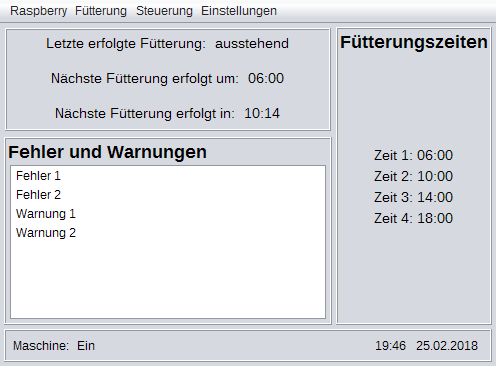
\includegraphics[width=0.60\textwidth]{Bilder/GUI/MainWindow}
  \end{center}
  \caption{MainWindow}
  \label{MainWindow}
  \vspace{-10pt}
\end{wrapfigure}
Das \textbf{MainWindow} besteht aus einer \textbf{Java JFrame Form}. In diesem Fenster wird dem Benutzer ein allgemeiner Überblick über die Anlage zur Verfügung gestellt. Somit können alle wichtigen Informationen schnell und leicht ersichtlich. Weiters ist das \textbf{MainWindow} das Hauptfenster des Programms. Über diese sind alle Dialog-,Steuerungs- und Informationsfenster erreichbar. Diese Fenster werden von Kapitel\ref{TimeManagement} bis Kapitel \ref{Update} genauer beschrieben. Das Aufrufen von anderen Fenseren ist über die Menüleiste, welche sich oben in der GUI befindet, möglich. 
\\ \\ Unter den Menüs der Menüleiste sind folgende Menüpunkte zu finden:
\begin{itemize}
\item[1] Raspberry
\begin{itemize}
\item[•] Neustarten
\item[•] Herunterfahren
\end{itemize}
\item[2] Fütterung
\begin{itemize}
\item[•] Einschalten/Ausschalten
\item[•] Fütterungszeiten verwalten
\end{itemize}
\item[3] Steuerung
\begin{itemize}
\item[•] manuelle Steuerung
\item[•] Positionsinformation
\end{itemize}
\item[4] Einstellungen
\begin{itemize}
\item[•] Update
\item[•] Benutzer anlegen
\item[•] WLAN
\item[•] Geräteinformation
\end{itemize}
\end{itemize}

\vspace{10pt}

Das \textbf{MainWindow} ist als Singleton implementiert. Somit wird ein nur Objekt des \textbf{MainWindow} erstellt. Das Singleton-Objekt wurde wie folgt erstellt:
\begin{lstlisting}[style=JavaStyle, caption=MainWindow createInstance()]
public static MainWindow createInstance()
    {
        if (instance != null)
        {
            throw new RuntimeException("intance already created");
        }

        if (!SwingUtilities.isEventDispatchThread())
        {
            throw new RuntimeException("not in EDT");
        }
        instance = new MainWindow();

        return instance;
    }
\end{lstlisting}
Diese Methode kann nur im EDT aufgerufen werden. Wenn diese Methode nicht im EDT aufgerufen wird oder das Objekt bereits besteht, wird ein jeweils eigener Error geworfen.
\\ \\ Diese Methode wird in der \textbf{main} Methode der Klasse wie folgt aufgerufen:
\begin{lstlisting}[style=JavaStyle, caption=MainWindow createInstance() Aufruf]
	java.awt.EventQueue.invokeLater(new Runnable()
        {
            @Override
            public void run()
            {
                MainWindow frame = MainWindow.createInstance();

            }
        });
\end{lstlisting}

Bis jetzt wurde der Singleton nur implementiert. Nun muss noch eine Methode implementiert werden um die \textbf{Instance} des Objekts abfragen zu können. Diese Methode sieht wie folgt aus:
\begin{lstlisting}[style=JavaStyle, caption=MainWindow.getInstance()]
public static MainWindow getInstance()
    {
        if (instance == null)
        {
            throw new RuntimeException("instance not created");
        }

        return instance;
    }
\end{lstlisting}

\vspace{10pt}

In der GUI werden je nach Maschinenstatus gewisse Funktionen blockiert. Folgende Funktionen sind blockiert, wenn die Fütterung aktiviert ist:
\begin{itemize}
\item[1] manuelle Steuerung
\item[2] Update
\end{itemize}
Das Blockieren das Funktionen wird mit folgender Methode gemacht:
\begin{lstlisting}[style=JavaStyle, caption=GUI Elemente blockieren]
private void updateGUIElements()
    {
        // control GUI elements depending on the machine state
        // update and manualControl not available while machine state = on 
        if (machineStateOn == true)
        {
            menu_update.setEnabled(false);
            menu_manualControl.setEnabled(false);
        }
        else
        {
            menu_update.setEnabled(true);
            menu_manualControl.setEnabled(true);
        }
    }
\end{lstlisting}

\newpage

\subsubsection{TimeManagement}\label{subsubsec:TimeManagement}
\begin{wrapfigure}{l}{0.65\textwidth}
\vspace{-20pt}
  \begin{center}
    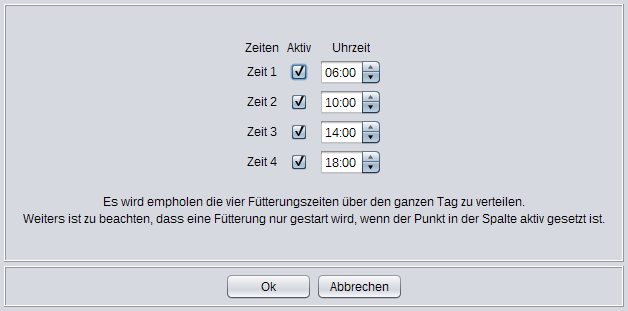
\includegraphics[width=0.65\textwidth]{Bilder/GUI/TimeManagement}
  \end{center}
  \caption{TimeManagement}
  \label{TimeManagement}
  \vspace{0pt}
\end{wrapfigure}
In der Klasse \textbf{TimeManagement} ist es dem Benutzer möglich alle Zeiten zu verwalten. Das GUI-Fenster dieser Klasse ist ein Dialogfenster. Bei Dialogfenstern ist es üblich, dass sie mit \textbf{Ok} und \textbf{Abbrechen} bedienbar sind.
\\ \\ Es können bis zu vier verschiedene Zeiten gewählt werden. Dabei müssen die Zeiten, bei Zeit 1 beginnend, aufsteigen angeordnet werden. Zusätzlich können Zeiten auch deaktiviert werden. Um eine Zeit zu deaktivieren muss das Häkchen vor der Zeit weggenommen werden.
\\ Wenn die Zeiten ausgewählt wurden, kann mit \textbf{Ok} bestätigt werden. Somit werden die Daten in das Programm übernommen und in die Datenbank gespeichert. Weiters schließt sich noch das Fenster.
\\ Falls\textbf{Abbrechen} gedrückt wird, werden die Änderungen nicht übernommen und das Fenster schließt sich.
\\ \\ Wenn das Dialogfenster im EDT aufgerufen wird, blockiert der EDT an dieser Stelle so lange, bis das Dialogfenster wieder geschlossen wird.

\newpage

Um in den Spinnern Uhrzeiten anzeigen zu lassen, müssen diese davor konfiguriert werden. Dazu muss im Designmodus der GUI Rechtsklick auf den Spinner gemacht werden. Weiters muss \textbf{Customize Code} ausgewählt werden. Anschließend öffnet sich folgendes Fenster: \\
\begin{wrapfigure}{l}{0.7\textwidth}
\vspace{-20pt}
  \begin{center}
    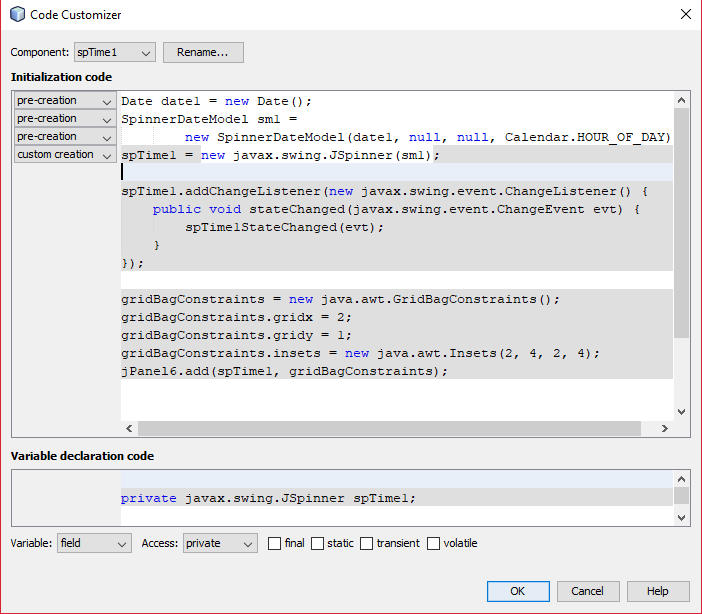
\includegraphics[width=0.70\textwidth]{Bilder/Java_Programm/SpinnerConfiguration}
  \end{center}
  \caption{Spinner Konfiguration}
  \label{SpinnerKonfiguration}
  \vspace{-70pt}
\end{wrapfigure}
\\ \\ In diesem Fenster ist der Code, welcher in den ersten vier Zeilen steht, hinzuzufügen. 
\\ Hier wird das Model für den Spinner gesetzt. Dieses Model gibt an, dass der Spinner ein Datum darstellen soll. Weiters wird nicht festgelegt was vom Datum angezeigt werden soll. Hier wird die Uhrzeit dargestellt. 
\\ \\ Diese Schritte sind für alle der vier verwendeten Spinner verwendet werden.

\vspace{60pt}

Zusätlich muss noch für jeden Spinner folgende Methode, im Constructor nach \textbf{initComponents();}, aufgerufen werden:
\begin{lstlisting}[style=Javastyle, caption=Spinner Zeitzone]
	JSpinner.DateEditor at1 = new JSpinner.DateEditor(spTime1, "HH:mm");
        	spTime1.setEditor(at1);
\end{lstlisting}

\vspace{10pt}

Im \textbf{Constructor} der \textbf{TimeManagement} Klasse werden, wenn das Fenster geöffnet wird, alle Spinner mit den momentanen Zeiten gefüllt. Zusätzlich werden noch die Häkchen, die festelegen ob eine Zeit aktiv ist, gesetzt.

\vspace{10pt}

Bevor das Fenster geschlossen wird, wenn \textbf{Abbrechen} gedrückt wird, wird überprüft, ob sich die Inhalte der Spinner veränder haben. Um dies zu überprüfen werden Events verwendet. Dafür wird für jeden Spinner das folgende Event verwendet:
\begin{lstlisting}[style=JavaStyle, caption=Spinner Event]
    private void spTime1StateChanged(javax.swing.event.ChangeEvent evt)                                     
    {                                         
        saved = false;
    }   
\end{lstlisting} 
Diese Event wird aufgerufen, wenn der Inhalt der Spinners verwendet wird. Dabei wird dann eine Boolean-Variable, die bekannt gibt, ob etwas verwendert wurde, auf \textbf{false} gesetzt. Wenn diese Boolean-Variable auf \textbf{false} ist, wird vor dem Beenden dem Benutzer eine Warnung ausgegeben, dass noch nicht gespeichert wurde. Zusätlich kann dann ausgwählt werden, ob wirklich ohne zu speichern beendet werden soll.
\\ \\ Wenn das Fenster mit \textbf{Ok} geschlossen wird, werden die Inhalte der Spinner, wenn sie geändert wurden, aus den Spinnern geholt. Zusätzlich wird das gleiche mit den ComboBoxes gemacht. Die Inhalte der Spinner und Comboxen werden anschließen in ein Dokument, also ein Format das für die Datenbank verständlich ist, gespeichert. Das Dokument sieht wie folgt aus:
\begin{lstlisting}[style=Javastyle, caption=Zeitendokument Getter-Methode]
// ... Code ...

newTimeDoc = new BasicDBObject("identifier", "Times")
                        .append("time1", time1)
                        .append("time1_active", time1_active)
                        .append("time2", time2)
                        .append("time2_active", time2_active)
                        .append("time3", time3)
                        .append("time3_active", time3_active)
                        .append("time4", time4)
                        .append("time4_active", time4_active);
\end{lstlisting}
Dieses Dokument wird anschließen mit folgender \textbf{Getter-Methode} geworfen damit sie in im \textbf{MainWindow} zugänglich ist:
\begin{lstlisting}[style=Javastyle, caption=Zeitendokument]
public BasicDBObject getNewTimeDoc()
    {
        return newTimeDoc;
    }
\end{lstlisting}

\newpage

\subsubsection{CreateUser}
\begin{wrapfigure}{l}{0.6\textwidth}
\vspace{-20pt}
  \begin{center}
    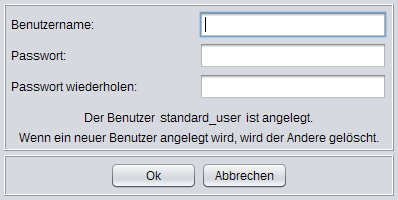
\includegraphics[width=0.60\textwidth]{Bilder/GUI/CreateUser}
  \end{center}
  \caption{CreateUser}
  \label{CreateUser}
  \vspace{-10pt}
\end{wrapfigure}
Die Klasse \textbf{CreateUser} bietet dem Benutzer die Möglichkeit einen Benutzer anzulegen. Mit dem angelegten Benutzer ist es möglich sich auf der Webseite der Anlage anzumelden. Die GUI ist in Abbildung \ref{CreateUser} zu sehen.
\\ Die GUI der Klasse ist ein Dialogfenster. Bei Dialogfenstern ist es üblich, dass sie mit \textbf{Ok} und \textbf{Abbrechen} bedienbar sind.
\\ \\ Es ist nur möglich einen Benutzer anzulegen. Wenn bereits ein Benutzer angelegt ist und dann ein Neuer angelegt wird, wird der alte Benutzer überschrieben. Um einen neuen Benutzer anzulegen müssen folgende Felder ausgefüllt werden: Benutzername, Passwort und Passwort wiederholen. Wenn eines dieser Felder leer gelassen wird, wird eine Fehlermeldung ausgegeben. Weiters wird eine Fehlermeldung ausgegeben, wenn die beiden Passwörter nicht übereinstimmen. Wenn alle drei Eingabefelder korrekt ausgefüllt wurden kann der Benutzer angelegt werden indem \textbf{Ok} gedrückt wird. Dadurch wird der Benutzer in das Programm übernommen und in die Datenbank gespeichert. Anschließend erscheint ein Informationsfenster welches den Benutzer darüber informiert, dass der Benutzer erfolgreich angelegt wurde. Danach schließt sich das Dialogfenster. Wenn anstatt von \textbf{Ok} \textbf{Abbrechen} gedrückt wird, schließt sich das Dialogfenster und die Änderungen werden verworfen.
\\ \\ Während das Dialogfenster geöffnet ist blockiert der EDT an der Stelle, an der das Dialogfenster geöffnet wurde.

\vspace{10pt}

Um das Passwort einzugeben wird ein \textbf{PasswordField} verwendet. Diese Eingabefeld wird speziell dazu verwendet Passwörter einzugeben. Eine Besonderheit davon ist, dass die Passwörter nicht als Text sonder als Sternchen dargestellt werden. Eine weitere ist, dass der Inhalt eine Zeichenkette ist, also ein Feld von Characters: \textbf{char[]}. Weiters unterscheided sich auch das Abfragen des Inhaltes im Vergleich mit eienm normalen Textfeld. Beim \textbf{PasswordField} kann der Inhalt mit \textbf{passwordField.getPassword()} abgefragt werden.
\\ \\ Um das Password im Programm besser verarbeiten zu können wird es wie folgt in einen String umformatiert:
\begin{lstlisting}[style=Javastyle, caption=char zu String]
	String string_password = valueOf(char_password);
\end{lstlisting}

\vspace{10pt}

Um eine gewisse Sicherheit zu gewährleisten wird das Password, bevor es in der Datenbank gespeichert wird, gehasht. Um das Password zu hashen wird der \textbf{SHA-512} verwendet. Im Programm wird das Passwort nur einmal gehasht. Falls die Katzenfütterungsanlage in Serie gehen sollte, sollte das Passwort öfters gehasht werden um die Sicherheit zu erhöhen.
\\ Das Password wurde wie folgt gehasht:
\begin{lstlisting}[style=Javastyle, caption=Hash Passwort]
	public static String hash(String passwordToHash, String salt)
    {
        String generatedPassword = null;
        try
        {
            MessageDigest md = MessageDigest.getInstance("SHA-512");
            md.update(salt.getBytes("UTF-8"));
            byte[] bytes = md.digest(passwordToHash.getBytes(StandardCharsets.UTF_8));
            StringBuilder sb = new StringBuilder();
            for (int i = 0;
                    i < bytes.length;
                    i++)
            {
                sb.append(Integer.toString((bytes[i] & 0xff) + 0x100, 16).substring(1));
            }
            generatedPassword = sb.toString();
        }
        catch (NoSuchAlgorithmException e)
        {
            e.printStackTrace();
        }
        catch (UnsupportedEncodingException ex)
        {
            Logger.getLogger(HashPassword.class.getName()).log(Level.SEVERE, null, ex);
        }
        return generatedPassword;
    }
\end{lstlisting}
Mit dem Parameter \textbf{String salt} kann noch ein String übergeben werden welcher vor dem Hashen des Passworts am Passwort angehänt wird. Somit wird die Entschlüsselung des Passwort nochmals erschwert und die Sicherheit erhöht sich.

\vspace{10pt}

Bevor das Fenster geschlossen wird, wenn \textbf{Update} gedrückt wird, wird überprüft, ob sich die Inhalte der Text- und Passwortfelder verändert haben. Dabei wird vom Event überwacht, ob in dem Feld ein neues Zeichen eingegeben wird. Danach wird eine Boolean-Variable, die angibt ob gespeichert wurde, auf \textbf{false} gesetzt. Das Event für das Textfeld sieht wie folgt aus:
\begin{lstlisting}[style=Javastyle, caption=Textfeld Event]
private void tfUser_nameKeyPressed(java.awt.event.KeyEvent evt)                                       
    {                                           
        saved = false;
    }
\end{lstlisting}
Wenn die Variable \textbf{false} ist, also noch nicht gespeichert wurde, wird dem Benutzer die Warnung ausgegeben werden, dass die veränderten Daten noch nicht gespeichert sind.

\vspace{10pt}

Wenn das Dialogfenster mit \textbf{Ok} bestätigt wird, wird das Benutzername und das Passwort in ein Dokument, welches für die Datenbank verständlich ist, gespeichert. Dieses Dokument sieht wie folgt aus:
\begin{lstlisting}[style=Javastyle, caption=Benutzerdokument]
newUserDoc = new BasicDBObject("identifier", "User").append("user_name", 
	user_name).append("user_password", hashedPassword);
\end{lstlisting}

Dieses Dokument wird anschließend noch mit einer \textbf{Getter-Methode} geworfen damit es im \textbf{MainWindow} zugägnlich ist:
\begin{lstlisting}[style=Javastyle, caption=Benutzerdokument Getter-Methode]
public BasicDBObject getNewUserDoc()
    {
        return newUserDoc;
    }
\end{lstlisting}

\subsubsection{ManualControl}
  \begin{figure}[H]
    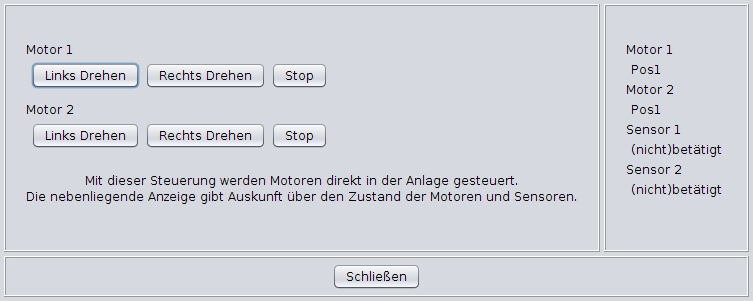
\includegraphics[width=0.90\textwidth]{Bilder/GUI/ManualControl}
    \caption{ManualControl}
  \label{ManualControl}
  \end{figure}
In der Klasse \textbf{ManualControl} wird eine manuelle Steuerung für die Motoren implementiert. Dies erleichtert dem Benutzer das Reinigen der Anlage, weil er zum Beispiel die Drehplatte, mit den Futterschüsseln, immer nachdrehen kann. Das gleiche gilt für das Förderband.
\\ Die GUI ist in Abbildung \ref{ManualControl} zu sehen.
\\ Die GUI der Klasse ist ein Steuerfenster. Da dieses Fenster ein Steuer- und kein Dialogfenster ist, werden kein \textbf{Ok} und \textbf{Abbrechen} benötigt. Aus diesem Grund ist nur ein Knopf \textbf{Schließen} vorhanden.

\vspace{10pt}

Wie beim Dialogfenster blockiert das Steuerfenster den EDT der Stelle wo es geöffnet wurde bis es wieder geschlossen wird.

\vspace{10pt}

Dieses Fenster ist aus Sicherheitsgründen nur dann aufrufbar, wenn der Maschinenzustand auf Aus ist. Der Grund dafür ist, dass es zu Fehlern kommen kann, wenn während einer Fütterung ein Motor ein oder aus geschalten wird.
\\ Weiters wird der Benutzer bevor er dieses Steuerfenster öffnet darüber infomiert, dass er nun direkt die Motoren steurt. Zusätlich wird der Benutzer gefragt ob er die Steuerung wirklick öffnen will.
\\ Der Benutzer kann nun beide Motoren unabhäging voneinander steuern. Er kann die Motoren in und gegen den Uhrzeigersinn drehen. Dazu muss er den Knopf mit der jeweiligen Drehrichtung im Steuerungsfenster klicken. Die Motoren sind mit dem jeweiligen Stop-Knopf wieder stopbar.
\\ Falls die Motoren vom Benutzer vor dem Schließen des Fensters nicht gestoppt werden, werden diese automatisch vom Programm gestopt. Dies dient dazu, dass sichergestellt ist, dass die Motoren immer gestopt werden.
\\ Die Methode zum Schließen des Fensters, welche auch die Motoren stopt, sieht wie folgt aus:
\begin{lstlisting}[style=JavaStyle, caption=Motoren stoppen und Fenster schließen]
	private void onSchließen(java.awt.event.ActionEvent evt)                                
    	{                                 
       		// stop engines when closing the conrtol dialog - security measurement
        	pi4j_instance.stopEngine1();
        	pi4j_instance.stopEngine2();
        
        	dispose();
    	} 
\end{lstlisting}

\vspace{10pt}

Neben dem Bereich für die Steuerung befindet sich noch ein Bereich in dem die Echtzeit-Zustände aller Motoren und Sensoren angezeigt werden. So kann der Benutzer ohne in die Anlage zu sehen feststellen, ob sich ein Motor dreht oder ein Sensor betätigt ist.

\vspace{10pt}

Die Motoren werden gesteuert, indem beim Drücken eines Knopfes, eine Methode aus dem \textbf{pi4j Singleton} (Kaptiel \ref{subsec:pi4j}) aufgerufen wird. Aus dieser Klasse ausgehend werden die Output-Pins und in weiterer Folge die Motoren gesteuert.
\\ Wenn ein Knopf gedrückt wird, wird die jeweilige zum Knopf gehörente Methode aufgerufen. Dies kann wie folt aussehen:
\begin{lstlisting}[style=JavaStyle, caption=Motoren drehen] 
	private void onMoveEngine1Counterclockwise(java.awt.event.ActionEvent evt)                                               
    	{                                                   
        	pi4j_instance.moveEngine1Counterclockwise();
    	}  
\end{lstlisting}

\vspace{10pt}

Um die aktuellen Positionen der Motoren und Zustände der Sensoren zu ermitteln und ausgeben wird ein SwingWorker verwendet. Dies ist unter Kapitel \ref{subsubsec:Positionsinformation} genauer beschrieben

\newpage

\subsubsection{Positionsinformation} \label{subsubsec:Positionsinformation}
\begin{wrapfigure}{l}{0.25\textwidth}
\vspace{-20pt}
  \begin{center}
    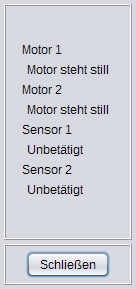
\includegraphics[width=0.25\textwidth]{Bilder/GUI/Positionsinformation}
  \end{center}
  \caption{Positionsinformation}
  \label{Positionsinformation}
  \vspace{-10pt}
\end{wrapfigure}
In der Klasse \textbf{Postionsinformation} wir dem Benutzer eine Übersicht über die Zustände der Motoren und Sensoren geboten. So kann er ohne direkt in die Anlage zu sehen festelleben, ob sich ein Motor dreht oder ein Sensor betätigt ist.
\\ Die GUI ist in Abbildung \ref{Positionsinformation} zu sehen.
\\ Die GUI der Klasse ist ein Informationsfenster. Da dieses Fenster kein Dialogfenster ist, werden \textbf{Ok} und \textbf{Abbrechen} nicht benötigt. Aus diesem Grund reicht ein Knopf \textbf{Schließen} aus.

\vspace{10pt}

Wie beim Dialogfenster blockiert das Informationsfenster den EDT an der Stelle wo es geöffnet wurde bis es wieder geschlossen wird.

\vspace{10pt}

Dieses Fenster ist, im Gegensatz zu \textbf{ManualControl}, auch aufrufbar, wenn die Fütterung aktiviert, also der Maschinenzustand auf \textbf{Ein}, ist.
\\ Bei der Anzeige für Drehrichtung der Motoren und die Zustände der Sensoren kann folgendes angezeigt werden:
\begin{itemize}
\item[1] Motoren
  \begin{itemize}
    \item[•] Motor steht still
    \item[•] Motor dreht links
    \item[•] Motor dreht rechts
  \end{itemize}
\item[2] Sensoren
  \begin{itemize}
    \item[•] Unbetätigt 
    \item[•] Betätigt 
  \end{itemize}
\end{itemize}

\vspace{10pt}

Die Drehrichtungen und die Zustände werden mithilfe des \textbf{pi4j Singleton} (Kapitel \ref{subsec:pi4j}) erfasst. In dieser Klasse sind Methoden implementiert, die diese Messungen durchführen können.
\\ Um dies annähernd echtzeitfähig zu realisieren wird ein SwingWorker verwendet. Im \textbf{doInBackground()} dieses SwingWorkers werden in einer Dauerschleife die Zuständer der Motoren und Sensoren abgefraft. Diese Zustände werden mit einem \textbf{publish()} an ein \textbf{process()} übergeben. Im \textbf{process()} werden die Zustände in die Label der GUI geschrieben.
\\ Das \textbf{process()} sieht wie folgt aus:
\begin{lstlisting}[style=JavaStyle, caption= Label aktualisieren]
	@Override
    protected void process(List<String[]> chunks)
    {
         String state[] = chunks.get((chunks.size() - 1));
            
         lbSensor1.setText(state[0]);
         lbSensor2.setText(state[1]);
         lbEngine1.setText(state[2]);
         lbEngine2.setText(state[3]);
    } 
\end{lstlisting}
Das \textbf{doInBackground()} ist wie folgt implementiert:
\begin{lstlisting}[style=JavaStyle, caption= Motor- und Sensorzustände ]
	@Override
        protected Object doInBackground() throws Exception
        {                        
            while (!isCancelled())
            {
                strSensor1 = pi4j_instance.statusSensor1();
                strSensor2 = pi4j_instance.statusSensor2();
                strEngine1 = pi4j_instance.statusEngine1();
                strEngine2 = pi4j_instance.statusEngine2();
                
                String state[] = null;
                state[0] = strSensor1;
                state[1] = strSensor2;
                state[2] = strEngine1;
                state[3] = strEngine2;
                
                publish(state);
                
                TimeUnit.MILLISECONDS.sleep(100);
            } 
            return 1;            
        }

\end{lstlisting}
In diesem \textbf{doInBackground()} werder  alle 100 Millisekunden die Motordrehrichtungen und die Sensorzustände abgefragt.

\newpage

\subsubsection{SystemInfo}
\begin{wrapfigure}{l}{0.40\textwidth}
\vspace{-20pt}
  \begin{center}
    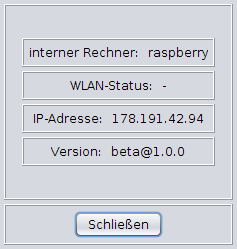
\includegraphics[width=0.40\textwidth]{Bilder/GUI/SystemInfo}
  \end{center}
  \caption{SystemInfo}
  \label{SystemInfo}
  \vspace{-10pt}
\end{wrapfigure}   
  text

\newpage

\subsubsection{Update}\label{subsubsec:Update}
\begin{figure}[H]
  \begin{minipage}[hbt]{0.45\textwidth}
    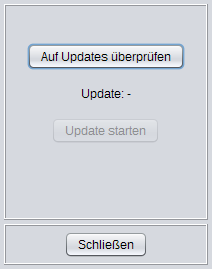
\includegraphics[width=0.9\textwidth]{Bilder/GUI/Update1}
 	\caption{Update suchen}
  	\label{Update}
  \end{minipage}
\hspace{.03\linewidth}
  \begin{minipage}[hbt]{0.45\textwidth}
    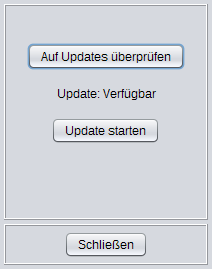
\includegraphics[width=0.9\textwidth]{Bilder/GUI/Update2}
  	\caption{Update verfügbar}
  	\label{Update2}
  \end{minipage}
  \vspace{0pt}
\end{figure}
Mit der \textbf{Update} Klasse ist es dem Benutzer möglich die Software seiner Anlage aktuell zu halten. Die GUI der Klasse ist auch ein Steuerfenster. Deswegen werden kein \textbf{Ok} und \textbf{Abbrechen} benötigt und es kann ein Knopf \textbf{Schließen} verwendet werden.

\vspace{10pt}

Wie beim Dialogfenster blockiert das Steuerfenster den EDT an der Stelle wo es geöffnet wurde bis es wieder geschlossen wird.

\vspace{10pt}

Wenn das Fenster aufgerufen wird, hat es das Aussehen aus der Abbildung \ref{Update}. Nun kann der Benutzer das Fenster schließen oder den Knopf \textbf{Auf Updates überprüfen} drücken. Sofern ein Update gefunden wird, wird der Knopf \textbf{Update starten} aktiviert und das Label ändert sich von \textbf{-} auf \textbf{Verfügbar}. Also sieht das Fenster aus wie in Abbildung \ref{Update2}.

\vspace{10pt}

Beim Überprüfen auf Updates wird die lokale Versionsnummer am Raspberry und die Versionsnummer am Repository überprüft. Wenn die Versionen nicht übereinstimmen ist ein Update verfügbar. Obwohl die Versionsnummer immer chronologisch nach oben gezählt wird, wird auch ein Update gemacht wenn die Versionsnummer niedriger wird. Der Grund dafür ist, wenn eine Version einmal einen schwerwiegenden Fehler beinhaltet, ist es ohne Probleme möglich auf die voherige Version zurück zu gehen. 

\vspace{10pt}

Die Daten für das Update werden von einem Git-Repository herunter geladen. Dies wird mit einem \textbf{git pull} Befehlt gemacht. Anschließend wird am Raspberry eine Datei bearbeitet, welche dem Raspberry beim Startet mitteilt, dass die Programme neu zu bauen sind. Nach jedem Update wird das Raspberry automatisch neu gestartet.

\vspace{10pt}

Wenn nun der Knopf \textbf{Update starten} gedrückt wird, wird folgende Funktion aufgerufen:
\begin{lstlisting}[style=JavaStyle, caption= Update]
    private void onUpdate(java.awt.event.ActionEvent evt)                          
    {                              
        try
        {
            Process process = Runtime.getRuntime().exec("git pull");
            process.waitFor();
            
            write("/home/"+System.getProperty("user.name")+"/git/fuettr/build");
            
            pTextUpdateErfolgreich.setVisible(true);
            
            Runtime.getRuntime().exec("sudo reboot");
        }
        catch (IOException ex)
        {
            Logger.getLogger(Update.class.getName()).log(Level.SEVERE, null, ex);
        }
        catch (InterruptedException ex)
        {
            Logger.getLogger(Update.class.getName()).log(Level.SEVERE, null, 
            "WaitFor ist interrupted");
        }        
    }
\end{lstlisting}
Der Pfad, der zum Speicherort der Datei führt, beinhaltet den Benutzernamen des Raspberrys. Deswegen wird die Methode \textbf{System.getProperty("user.name")} verwendet, um den aktuellen Benutzernamen herauszufinden.

\newpage

\section{Zusammenfassung/Verbesserungsmöglichkeiten}
\subsection{Probleme mit Mongodb am Raspberry}
\subsection{Probleme mit pi4j -> Snapshotversion verwendet - ansonsten werden pins nicht erkannt}
\subsection{GUI auf "Touchscreen-Design" abändern}
\subsection{Besser Benutzerverwaltung - Mehrere Benutzer anlegen}
\subsection{Selbst erstellbare Vorlagen in denen Zeiten gespeichert werden}

\chapter{Teil 1 Mechanik}
\section{Einleitung}
\section{Aufgabenstellung}
\subsection{Zielsetzung}
\subsection{Problematik}
\newpage
\section{Konzepte} 

\subsection{Variante 1} 
\subsubsection{Übersicht der Prozessschritte}
\begin{itemize}
\item[1] Füllen des Futtermagazins
\item[2] Führen zur Schneidplatte
\item[3] Schnitt
\item[4] Pressen
\item[5] Entsorgen
\item[6] Füttern
\end{itemize}

\subsubsection{Füllen des Futtermagazins}

Im den folgenden Bildern wird mithilfe einer Lego-Darstellung gezeigt, wie das Magazin aus verschiedenen Blickwinkeln befüllt aussieht. Hier muss man beachten das die vom Hersteller zu öffneten Seite in Richtung des Schneidewerks zeigt (die schmale Seite mit der Einkerbung). Das ganze Förderband besteht grundsetzlich aus der Halterung die das Magazin in einer bestimmten Höhe hält, damit die einzelnen Trennwände nicht mit dem Boden kollidieren und somit keine freie Bewegung ermöglicht ist. Der Oberteil des Bandes schließt eben mit der Schneideplattehöhe ab um ein leichtes gleiten der Packung durch den Greifer zu ermöglichen, ohne das es Höhenunterschiede überwinden muss. Weiters wird über zwei Räder ein Band gespannt an denen die Wände in Abstand der Dicke der Packung festgemacht werden. Das Band wird mithilfe eines Motors in Bewegung gebracht und kann somit von Abteil zu Abteil bewegt werden um immer nach dem füttern eine neue Packung bereit zu stellen. Auf diesem Band können je nach Länge eine gewissen Anzahl an Futterpackung gelegt werden, natürlich nur auf der Oberseite da die Packungen ansonsten aus den Abteilungefallen fallen, weil sie nicht nach oben geschlossen sind.  Siehe Abbildungen: \ref{Magazin Vorne}, \ref{Magazin Seitlich}, \ref{Magazin Oben}

\begin{figure}[H]
\begin{center}
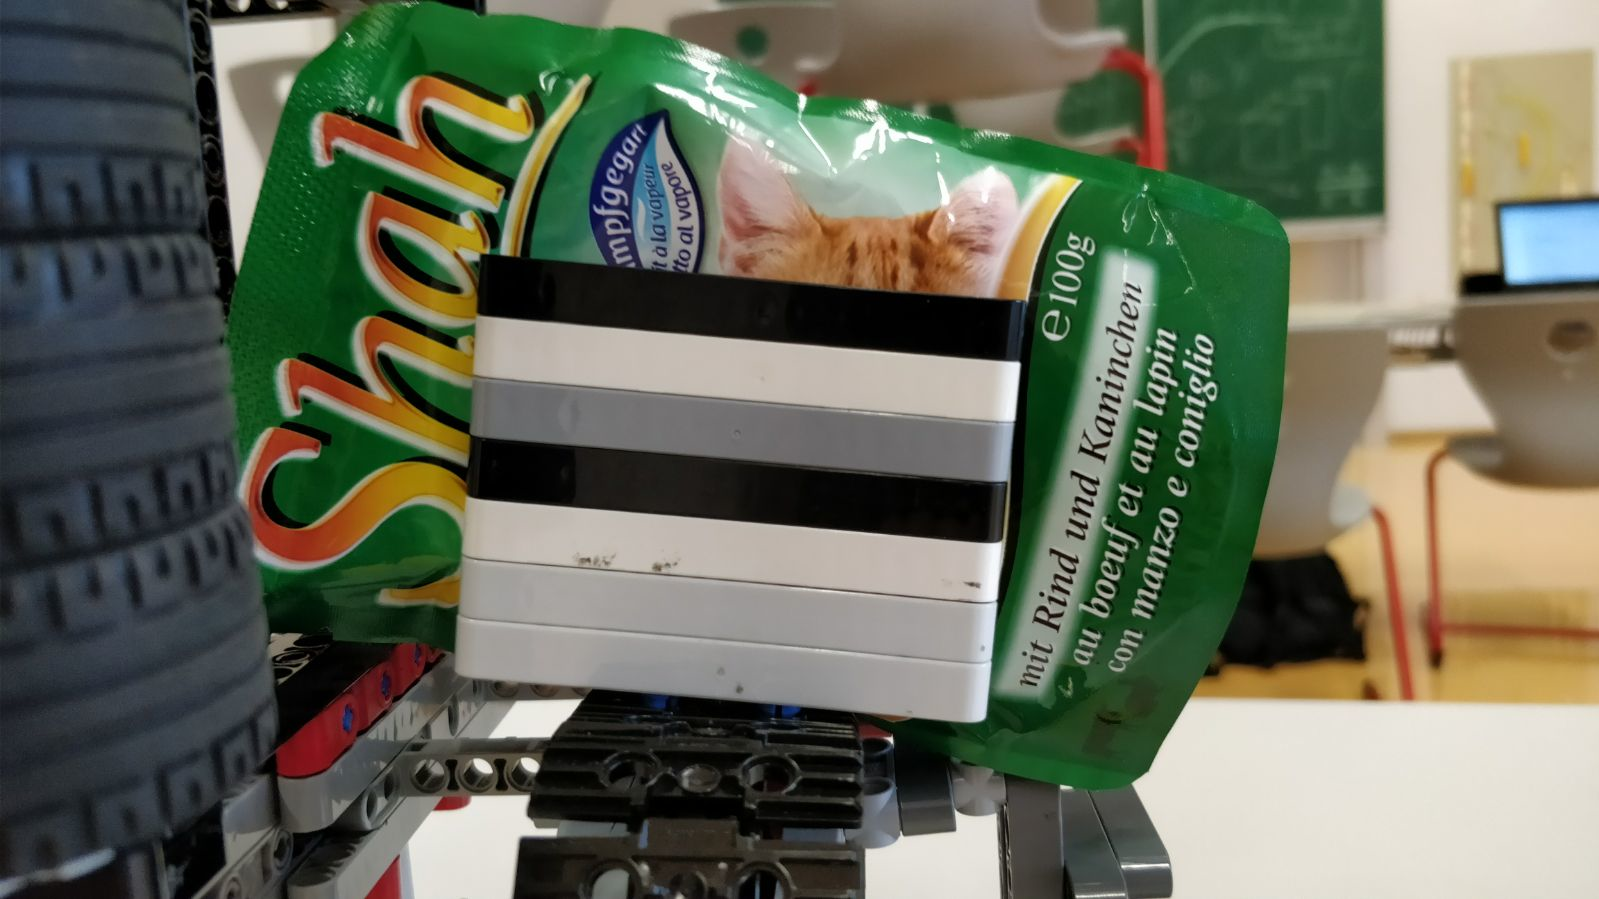
\includegraphics[width=13cm]{Bilder/Ablauf_1_png/Magazin_Vorne.png}
\caption{Magazin Vorne}
\label{Magazin Vorne}
\end{center}
\end{figure}

\begin{figure}[H]
\begin{center}
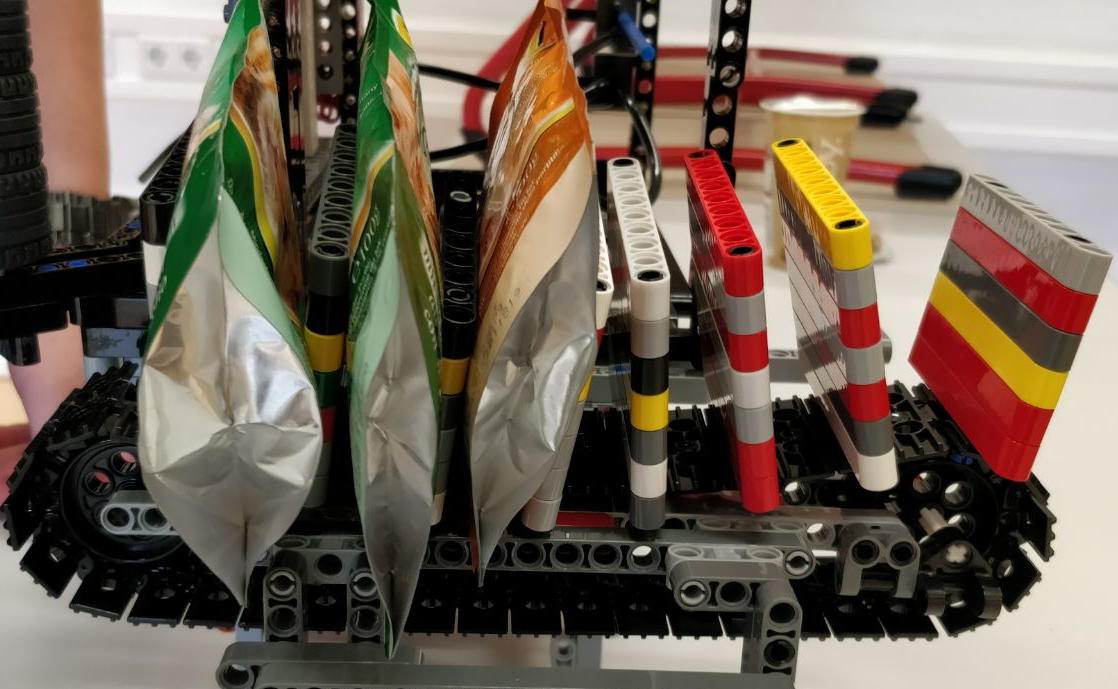
\includegraphics[width=13cm]{Bilder/Ablauf_1_png/Magazin_Seitlich.png}
\caption{Magazin Seitlich}
\label{Magazin Seitlich}
\end{center}
\end{figure}

\begin{figure}[H]
\begin{center}
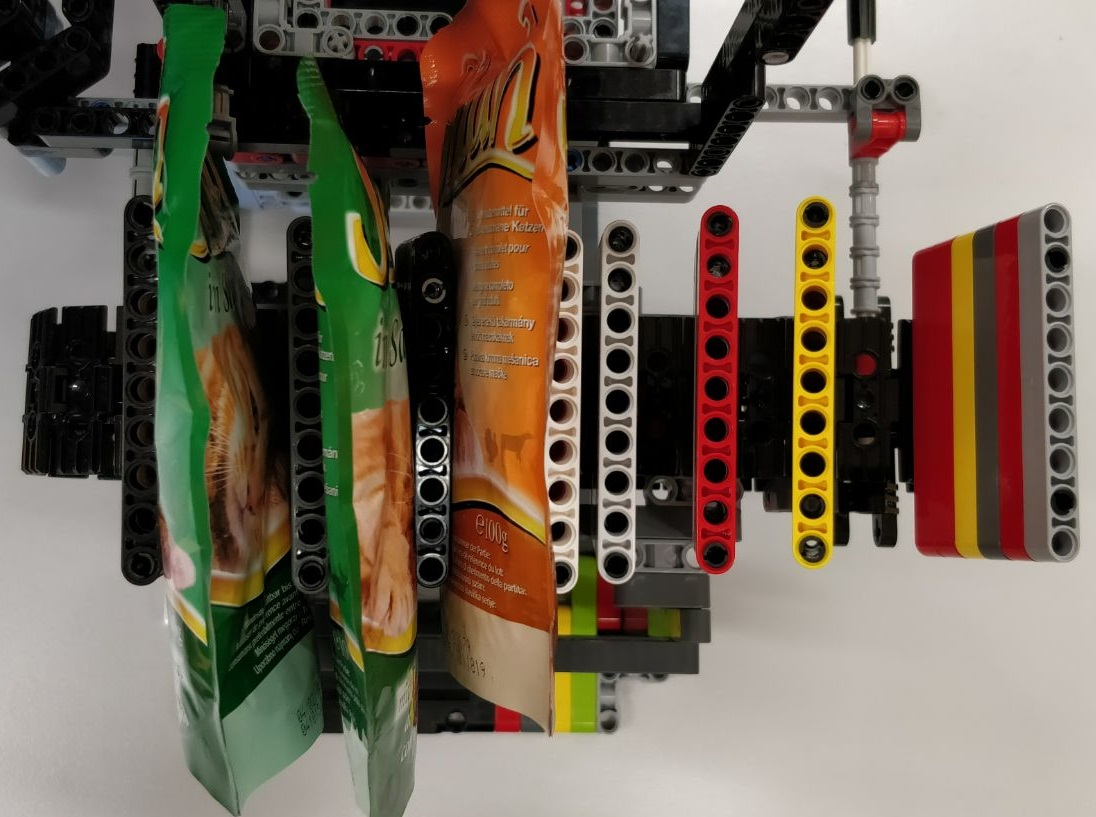
\includegraphics[width=13cm]{Bilder/Ablauf_1_png/Magazin_Oben.jpeg}
\caption{Magazin Oben}
\label{Magazin Oben}
\end{center}
\end{figure}

\subsubsection{Führen zur Schneidplatte}

In diesem Schritt wird mithilfe eines Greifers (dargestellt durch eine Hand) die Packung in richtiger Position gebracht.
Durch die richtige Höhe des Förderbandes muss der Greifer keine hohe Kraft besitzen um die Packung an ihrem Zielort zu bringen. Der Greifer dient auch noch dazu während des Schneidens neben den Magentzylindern die Packung stabil an Stelle zu halten ohne dass der Schnittpunkt verrutscht und die Schneide nicht mehr die Einkerbung, die leichter zu Schneiden ist, trifft. Das kann zu dem Problem führen, dass man die dickere Kunstoffumhüllung schneidet und der Schnitt nicht Ordnungsgemäß durchgeführt wird. Dadurch kann der Kunstoff zwischen die Schneiden gelangen und sie damit auseinander drücken. Dadurch kann die Packung nicht aufgeschnitten werden. Siehe Abbildungen: \ref{Magazin Auszug}, \ref{Magazin Mitte}

\begin{figure}[H]
\begin{center}
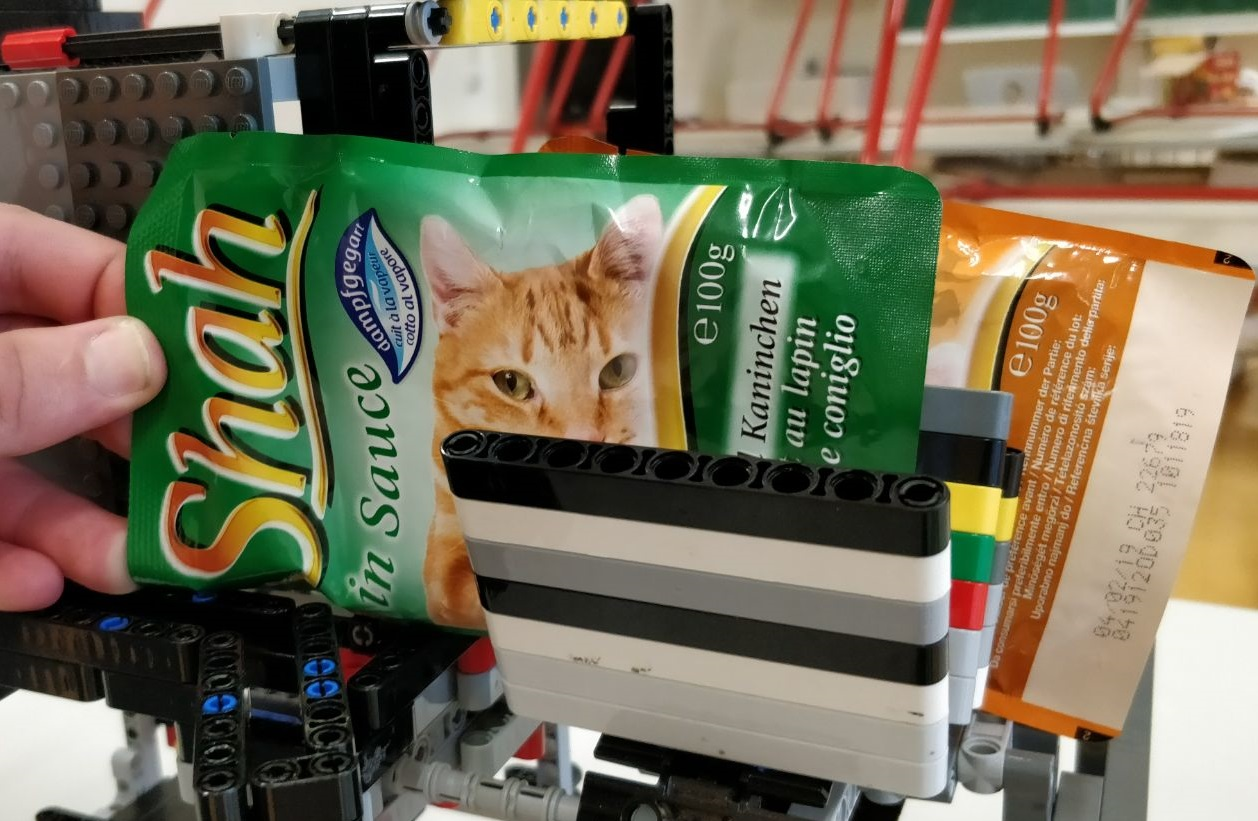
\includegraphics[width=13cm]{Bilder/Ablauf_1_png/Magazin_Auszug.jpeg}
\caption{Magazin Auszug}
\label{Magazin Auszug}
\end{center}
\end{figure}

\begin{figure}[H]
\begin{center}
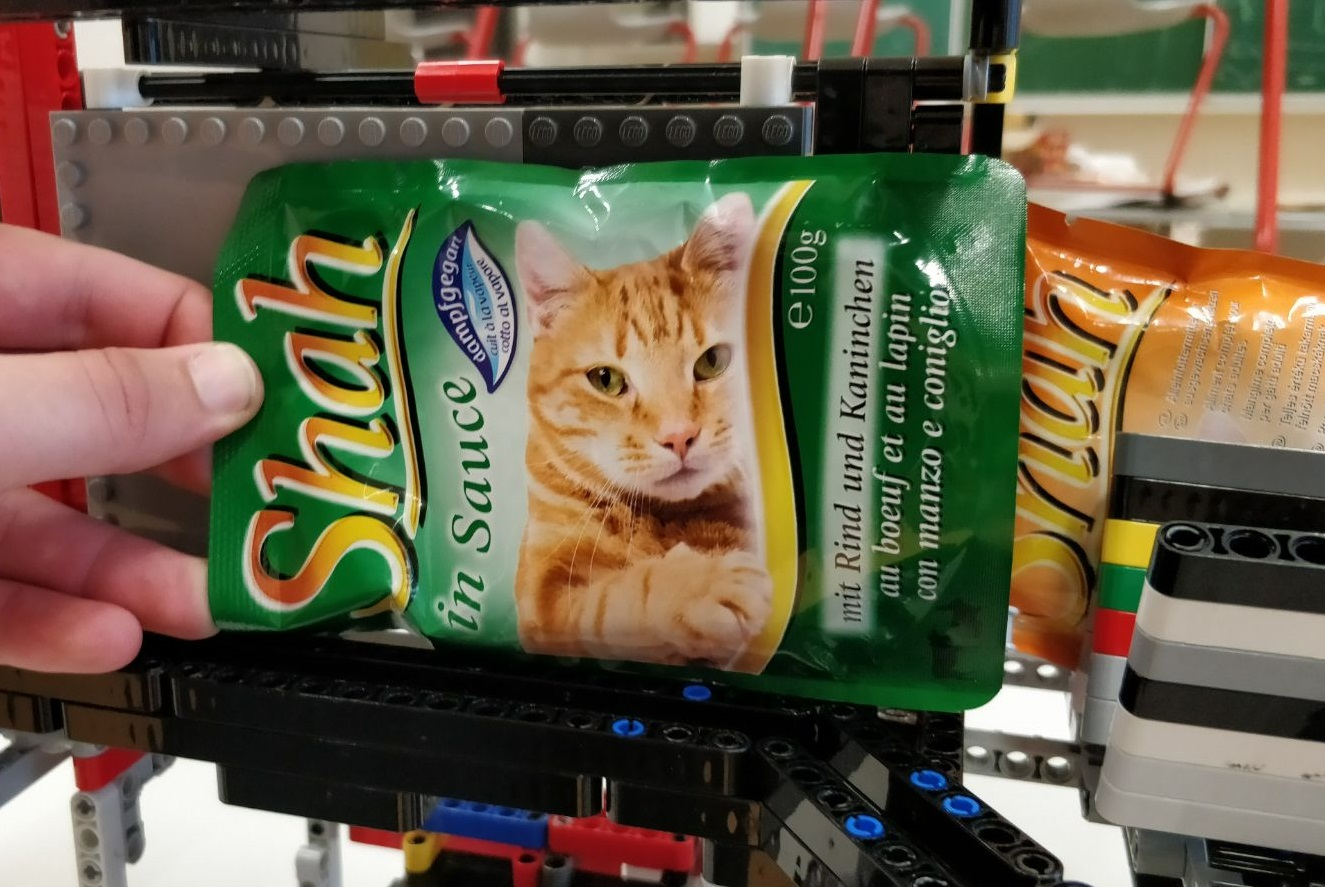
\includegraphics[width=13cm]{Bilder/Ablauf_1_png/Magazin_Auszug_2.jpeg}
\caption{Magazin Auszug Mitte}
\label{Magazin Mitte}
\end{center}
\end{figure}

Wie im Bild gezeigt liegt das Katzenfutterpackerl in der richtigen Position und wird mit zwei Magnetzylindern an der Schneidefläche festgehalten. Die Magnetzylinder haben genügend Kraft um die Packung auch während dem Schnitt und der Walzphase in Position zu halten. Wenn die Packung verrutschen würde könnte im schlimmsten Fall die Funktion der Maschine beeinflusst werden, indem sie den Greifer oder das Förderband blockiert. Daraufhin muss die Maschine manuell geöffnet und den Beutel per Hand rausgeholt werden. Siehe Abbildung: \ref{Schneidebereit}

\begin{figure}[H]
\begin{center}
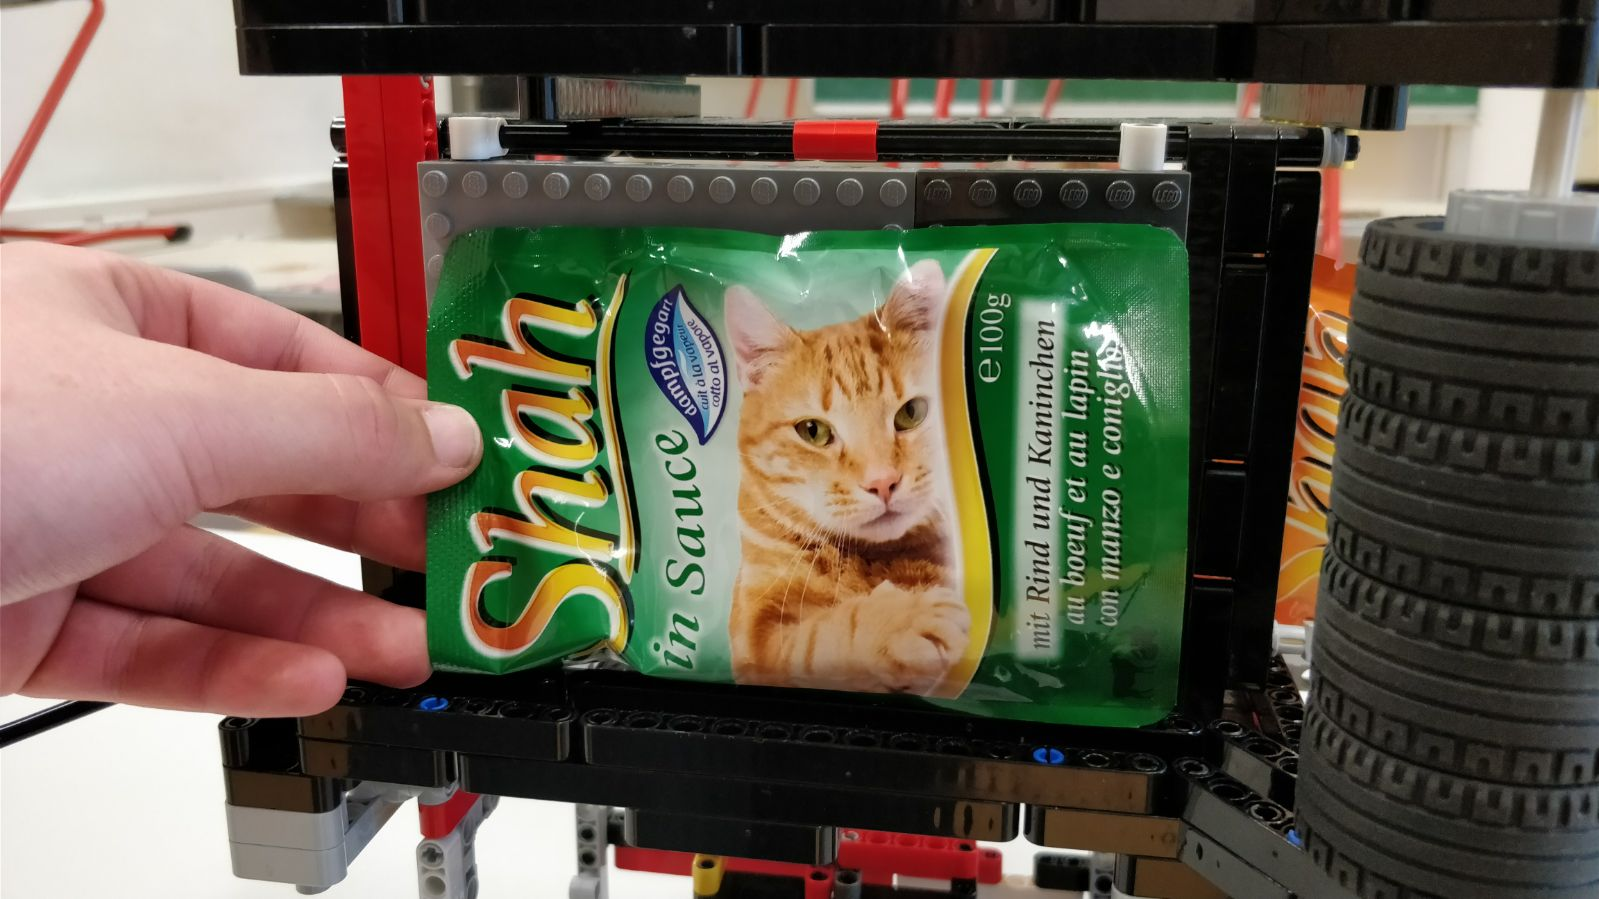
\includegraphics[width=13cm]{Bilder/Ablauf_1_png/Schneidebereit.jpeg}
\caption{Schneidebereit}
\label{Schneidebereit}
\end{center}
\end{figure}

\subsubsection{Schnitt}

In der richtigen Position muss man mit 2 scharfen Klingen mit viel Druck die Packung aufschneiden. Eine davon wird an der Schnittfläche angebracht und die andere macht die Schneidbewegung, wobei die beiden aneinander reibenden Kanten in einem Schnitt resultieren. Die Packung kann mit einem Schnitt vollständig geöffnet werden. Mit zu wenig Druck gelangt zu viel Kunstoffmaterial zwischen die Schneideflächen und durch die Länge der Schneiden biegen sie sich auseinander und somit kommt kein ordentlicher Schnitt zusammen. Bei öffteren Auftritts dieses besprochenen Problems bei der selben Packung kann es zufolge haben, dass sich die Packung nicht mehr mit der Maschine schneiden lässt, weil es sich durch die vielen Versuche verformt.  Siehe Abbildung: \ref{Schnitt}

\begin{figure}[H]
\begin{center}
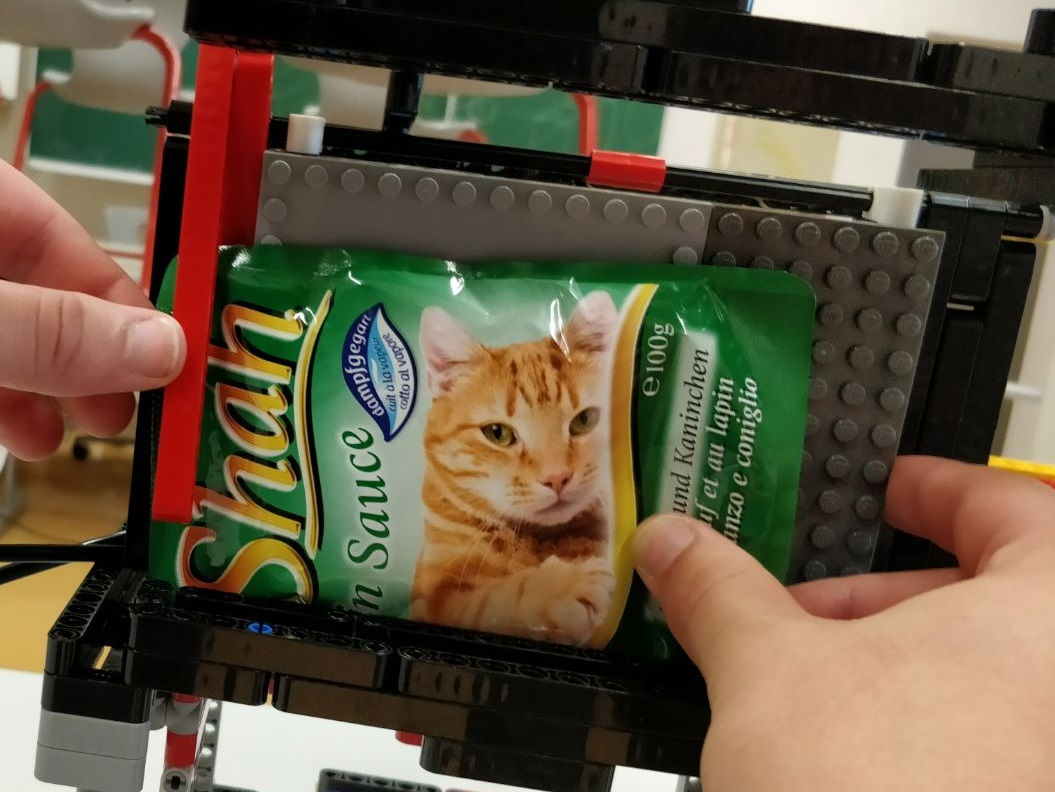
\includegraphics[width=13cm]{Bilder/Ablauf_1_png/Schnitt}
\caption{Schnitt}
\label{Schnitt}
\end{center}
\end{figure} 

\subsubsection{Pressen}

Nach dem Aufschneiden wird mit einer Rolle die Packung ausgepresst. Dazu werden zuerst die ersten 2 Magnetzylinder gelöst bis die Rolle vorbei ist. Danach werden sie wieder in Position gebracht. Daraufhin werden die anderen beiden gelöst und die Rolle fährt ans Ende. Die Rolle ist auf einer Welle plaziert, diese wird mit 2 Sicherrungsringen an einer  vorgegebenen Position befestigt. Die Rolle ist 10 cm breit, damit ohne Probleme die 9,4cm breite Futterpackung ausgepresst werden kann. Sie wird in einer Vorrichtung an der Maschine angehängt und steht mit einem bestimmten Winkel auf die Schneidfläche damit ein großer Anpressdruck entsteht. Durch die schmierige Konsistenz gleitet das Futter aus der Verpackung und wird nicht von der Walze zermatscht. Nach der Beseitigung der Verpackung werden zuerst die beiden Magnetzylinder von der Maschine entfernt in Anfangsposition gebracht, damit die Walze ohne Hinternis in Startposition zurückkehren kann. Siehe Abbildungen: \ref{Ausquetschen Beginn}, \ref{Ausquetschen Mitte}, \ref{Ausquetschen Ende}

\begin{figure}[H]
\begin{center}
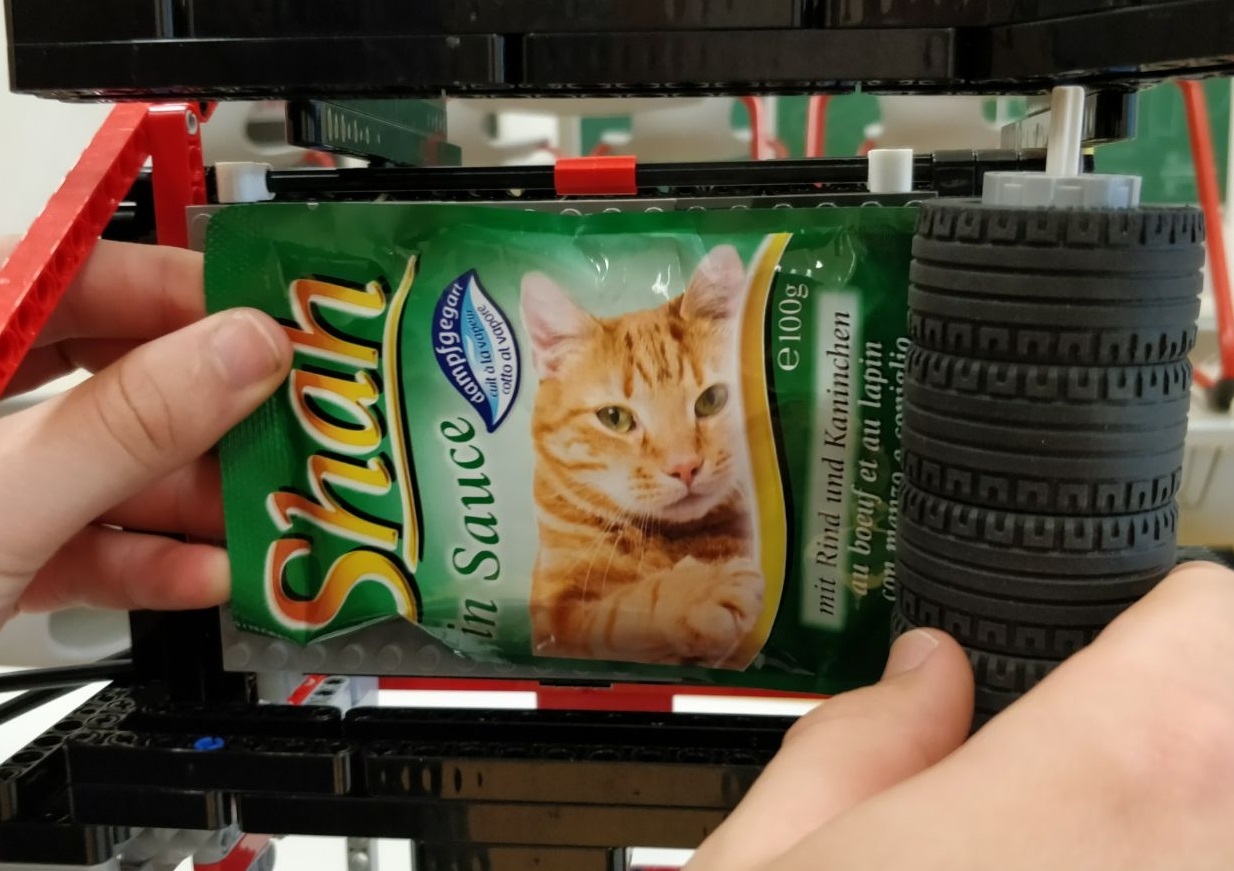
\includegraphics[width=13cm]{Bilder/Ablauf_1_png/Ausquetschen_1}
\caption{Ausquetschen Beginn}
\label{Ausquetschen Beginn}
\end{center}
\end{figure}

\begin{figure}[H]
\begin{center}
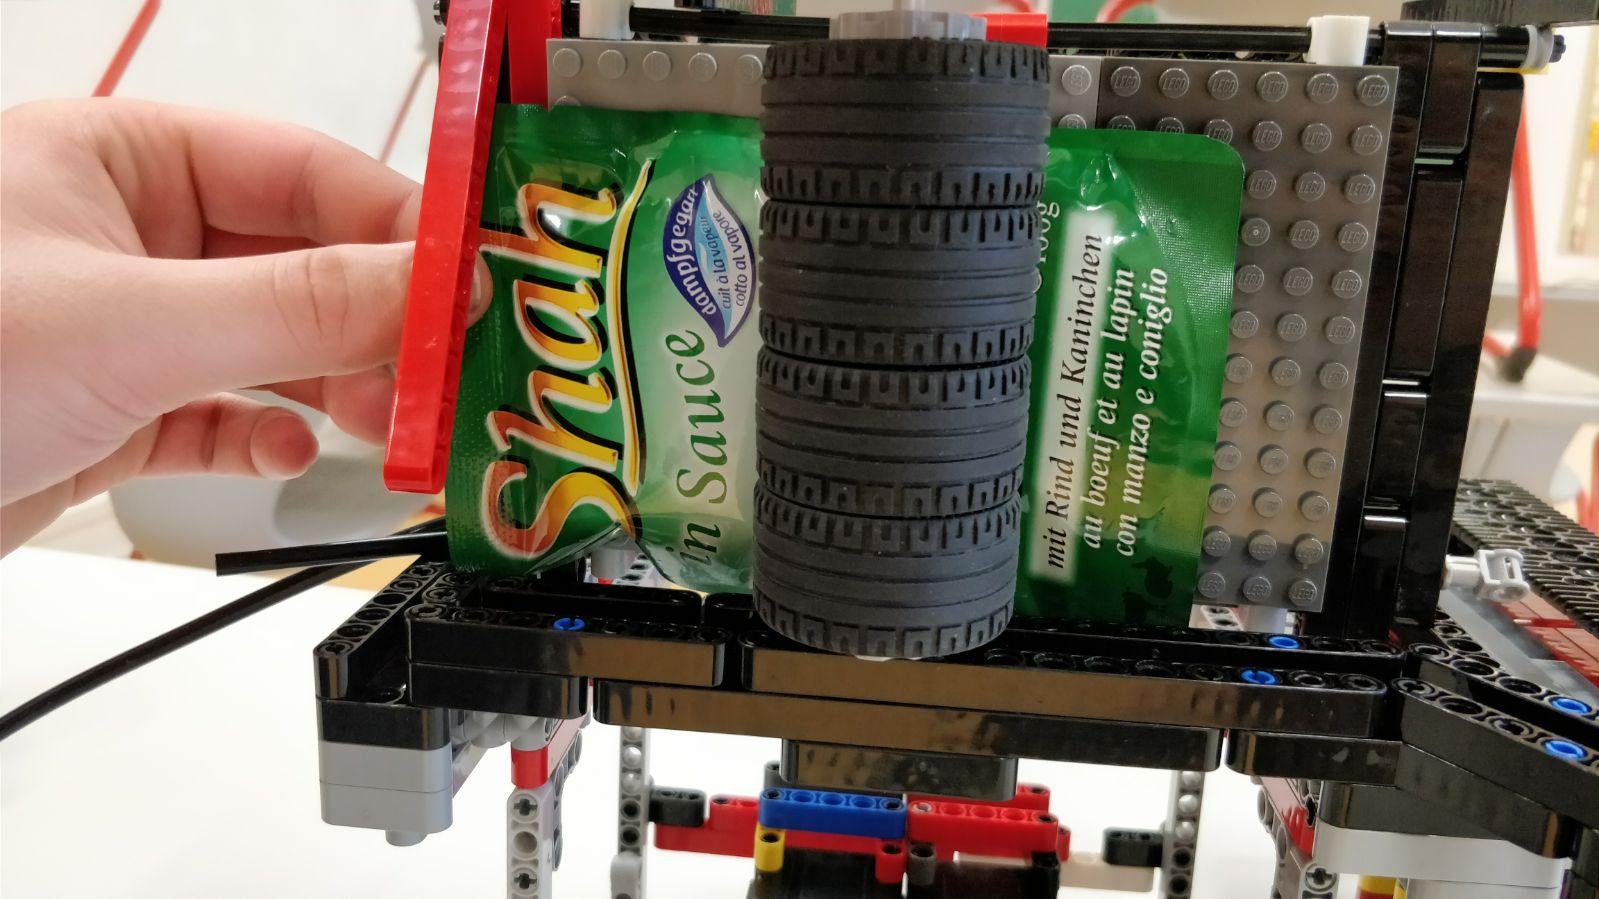
\includegraphics[width=13cm]{Bilder/Ablauf_1_png/Ausquetschen_2}
\caption{Ausquetschen Mitte}
\label{Ausquetschen Mitte}
\end{center}
\end{figure}

\begin{figure}[H]
\begin{center}
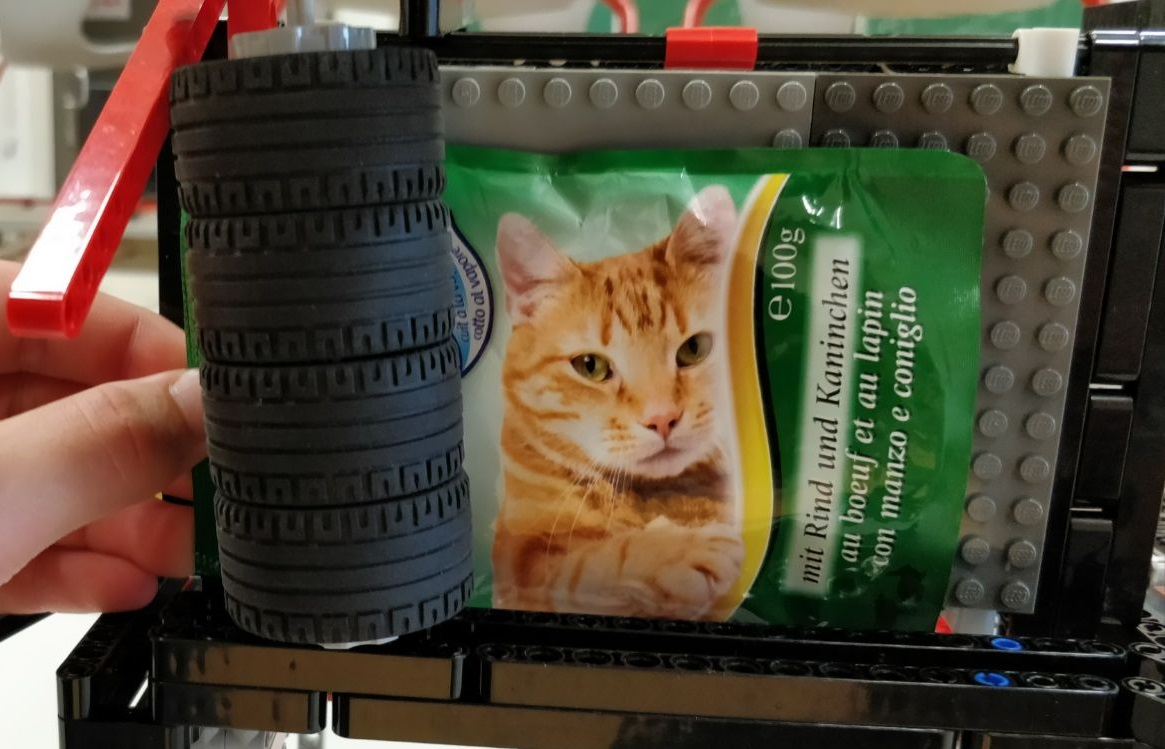
\includegraphics[width=13cm]{Bilder/Ablauf_1_png/Ausquetschen_3}
\caption{Ausquetschen Ende}
\label{Ausquetschen Ende}
\end{center}
\end{figure}
\newpage
\subsubsection{Entsorgen}

Nach dem Auspressen wird die leere Packung durch die Rückklappe in einen Luftdichten Container geworfen. Die Klappe wird durch zwei Stifte gehalten und lässt sich durch ein Scharnier nach hinten klappen.  Siehe Abbildung: \ref{Auswurf Beginn}, \ref{Fertiger Auswurf}

\begin{figure}[H]
\begin{center}
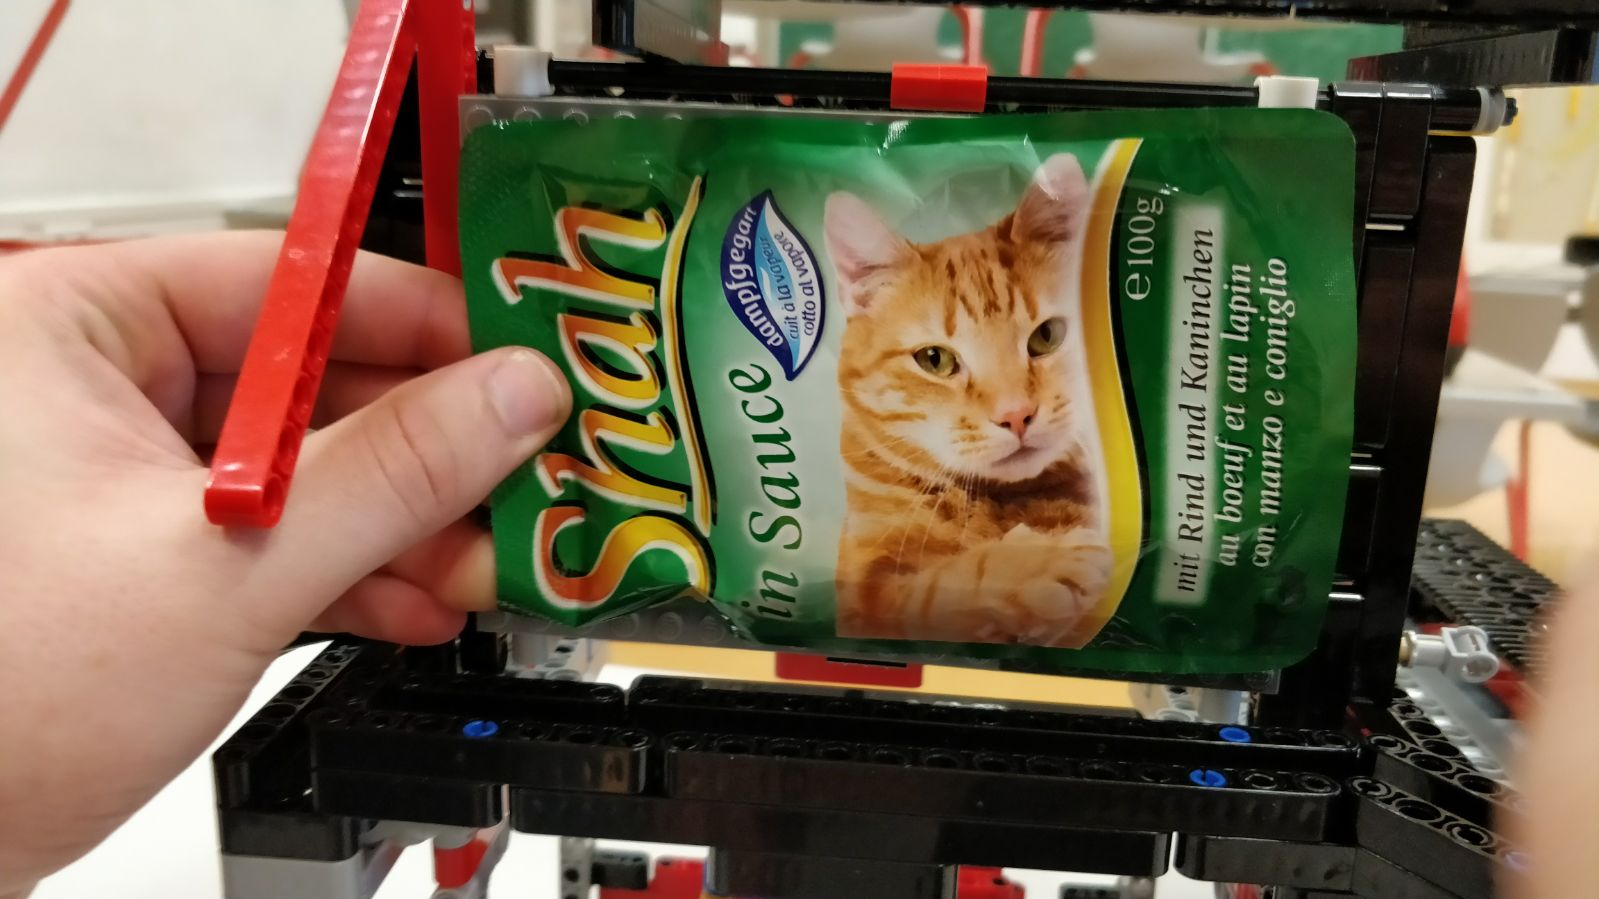
\includegraphics[width=13cm]{Bilder/Ablauf_1_png/Auswurf_1}
\caption{Auswurf Beginn}
\label{Auswurf Beginn}
\end{center}
\end{figure}

In der Abbildung: \ref{Bolzen drinnen} sieht man den Stift der ein vorzeitiges nach Hinten klappen verhindert.

\begin{figure}[H]
\begin{center}
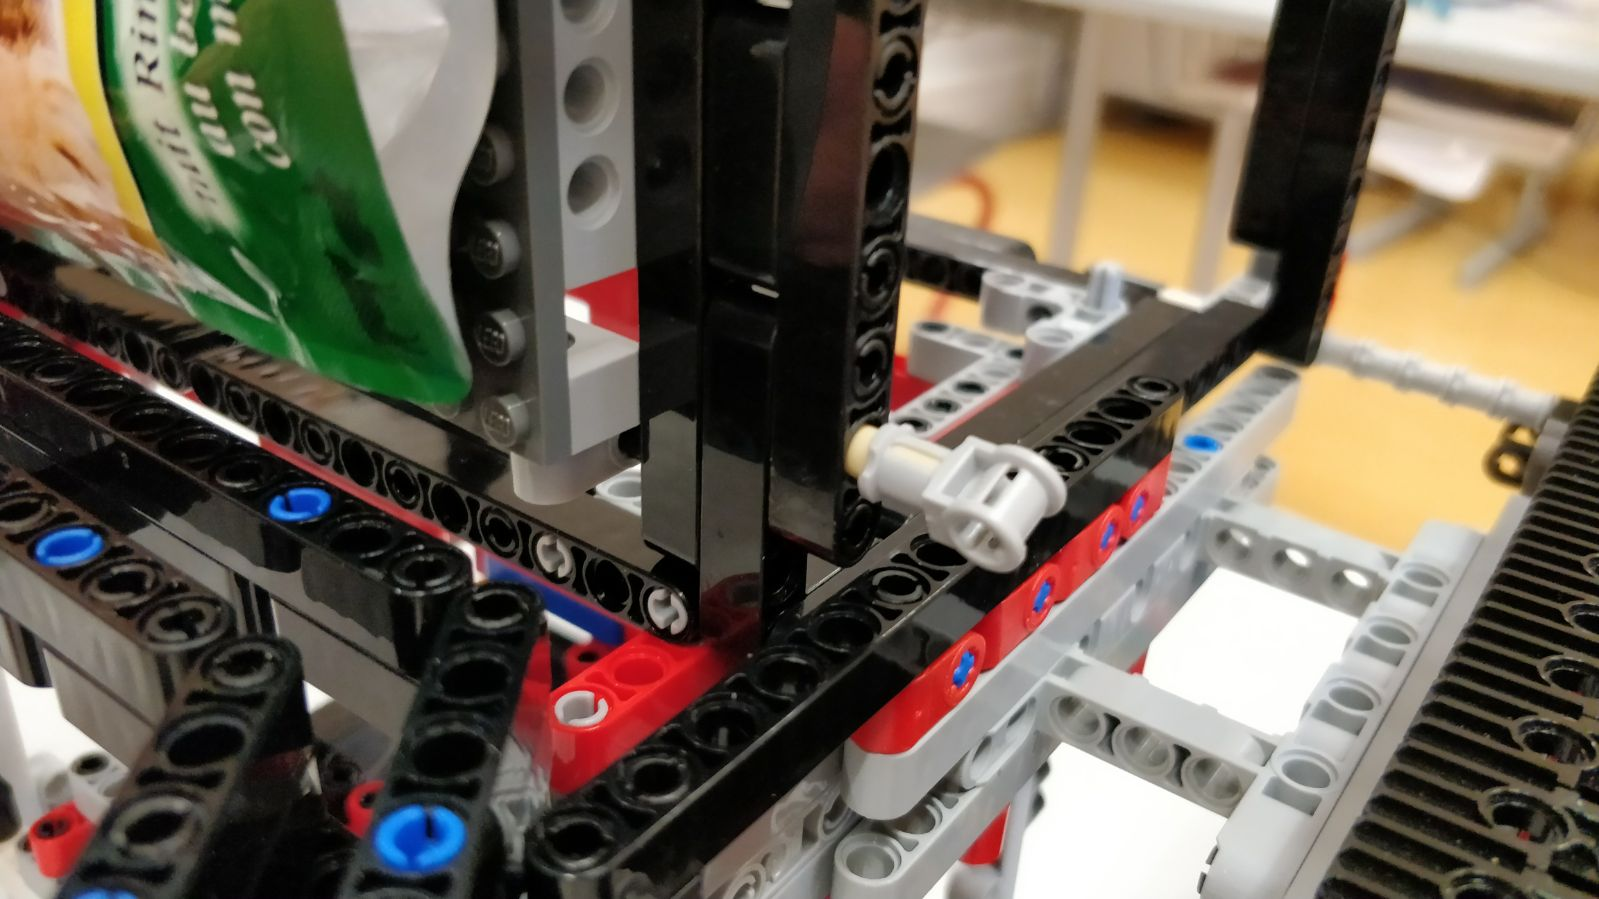
\includegraphics[width=13cm]{Bilder/Ablauf_1_png/Auswurf_2}
\caption{Bolzen drinnen}
\label{Bolzen drinnen}
\end{center}
\end{figure}


In der Abbildung: \ref{Bolzen entfernen} wurde der Bolzen entfernt und somit lässt sich die Klappe nach hinten klappen.

\begin{figure}[H]
\begin{center}
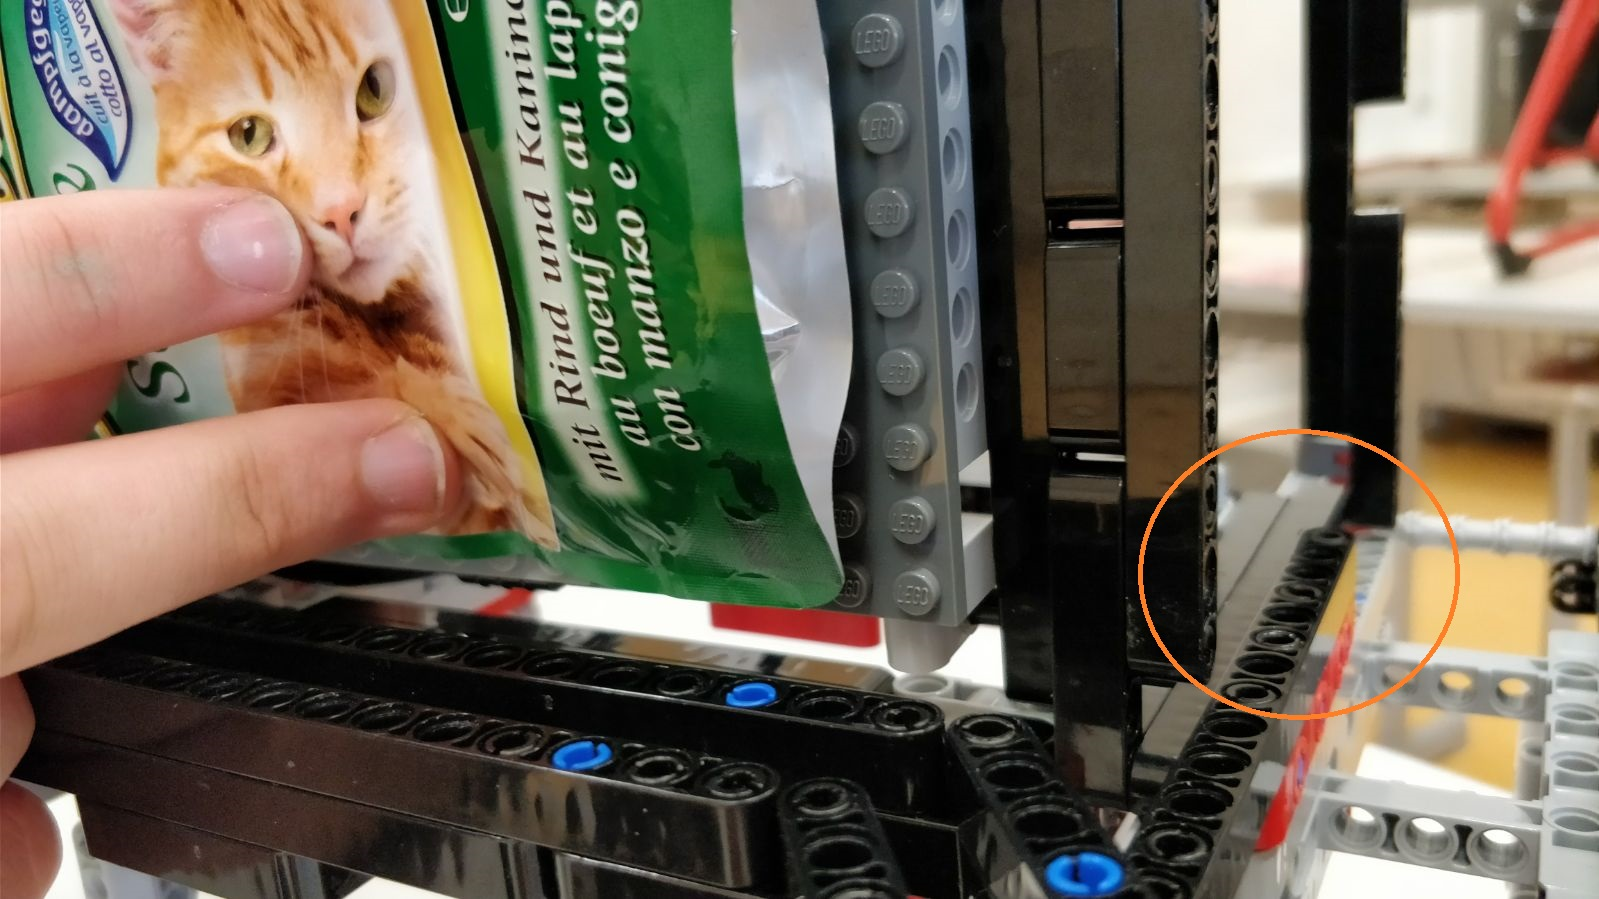
\includegraphics[width=13cm]{Bilder/Ablauf_1_png/Auswurf_3}
\caption{Bolzen entfernen}
\label{Bolzen entfernen}
\end{center}
\end{figure}

In der Abbildung: \ref{Klappe öffnen} wird demonstriert wie die Magnetzylinder die leere Packung gegen die Klappe drücken, wodurch die Klappe sich öffnet.

\begin{figure}[H]
\begin{center}
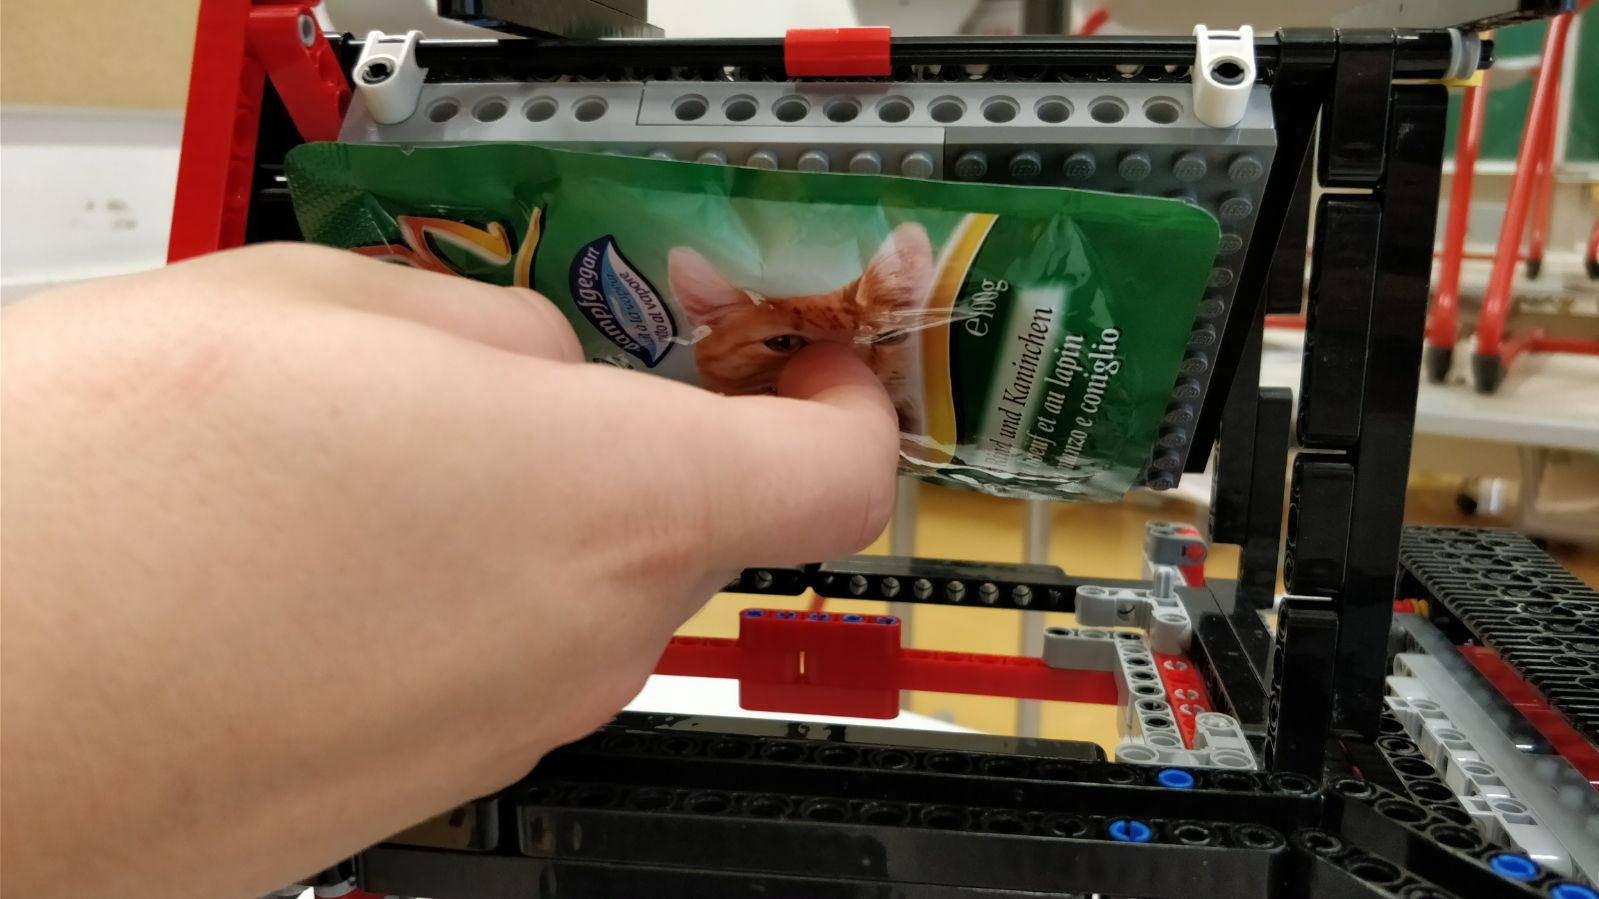
\includegraphics[width=13cm]{Bilder/Ablauf_1_png/Auswurf_4}
\caption{Klappe öffnen}
\label{Klappe öffnen}
\end{center}
\end{figure}

\begin{figure}[H]
\begin{center}
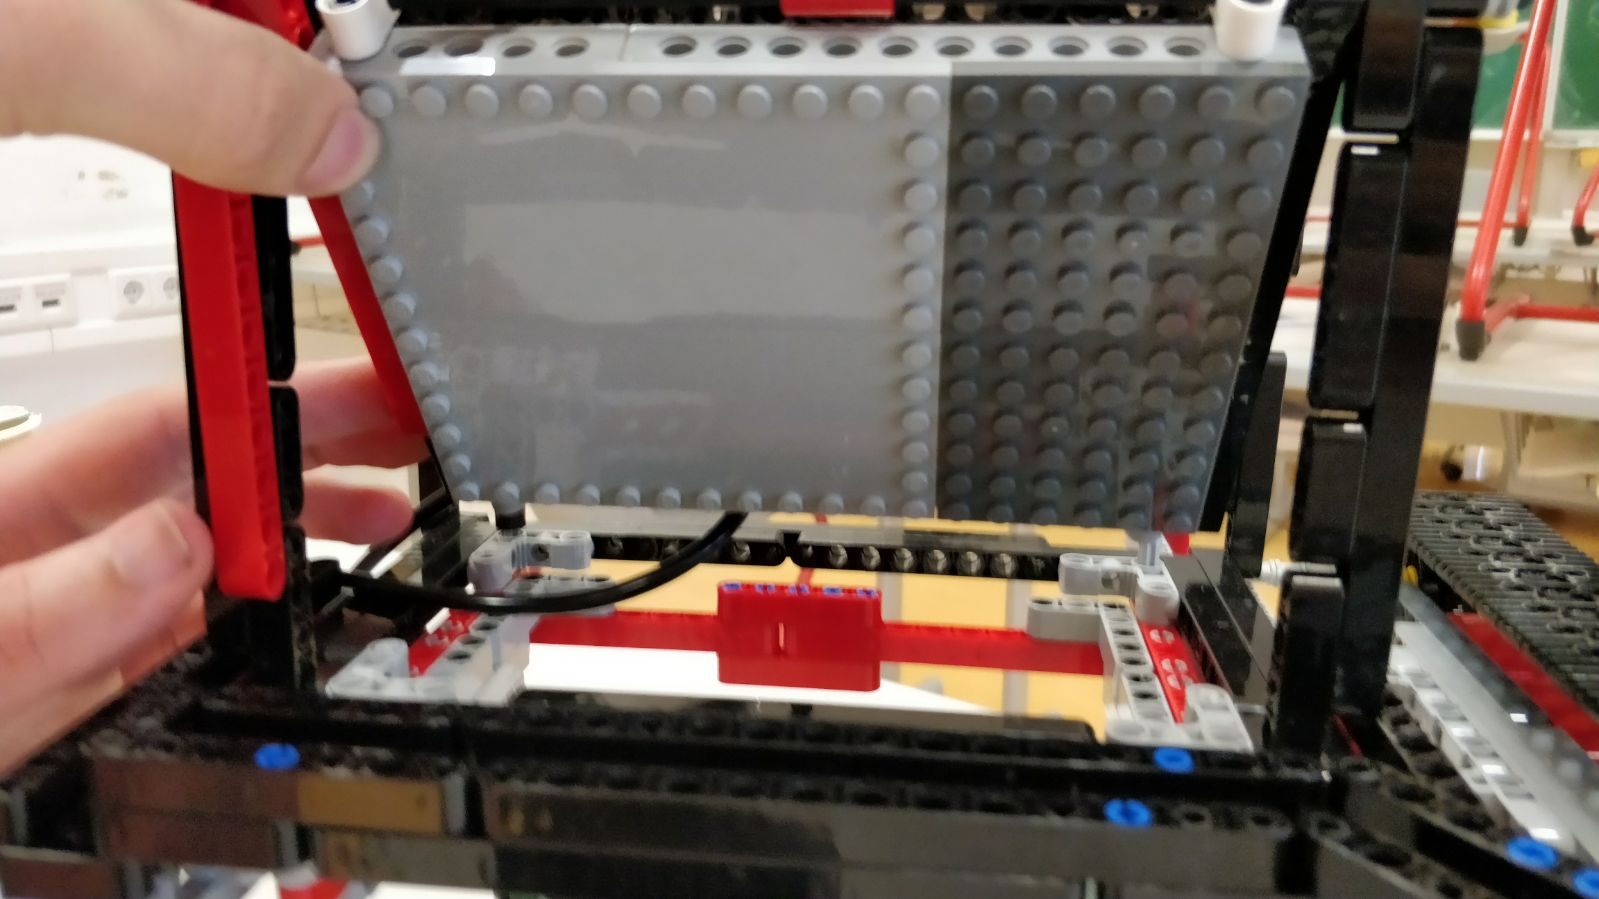
\includegraphics[width=13cm]{Bilder/Ablauf_1_png/Auswurf_5}
\caption{Fertiger Auswurf}
\label{Fertiger Auswurf}
\end{center}
\end{figure}

\subsubsection{Füttern}

\begin{wrapfigure}{r}{0.5\textwidth}
\vspace{-40pt}
  \begin{center}
    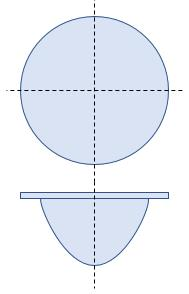
\includegraphics[width=0.17\textwidth]{Bilder/Powerpoint/Loch_Futterschuessel}
  \end{center}
  \caption{Loch Futterschüssel}
  \label{Loch_Futterschuessel}
  \vspace{-10pt}
\end{wrapfigure}

Die Maschine besitzt 5 Futterschüsseln die auf einer drehbaren Platte stehen. Vor dem Füttern wird eine saubere Platte unter der Stelle, wo später die Packung aufgeschnitten wird, positioniert. Während es ausgepresst wird, fliegt das Futter in die Futterschüssel. Wenn der Auspressvorgang beendet ist, wird die Futterschüssel an eine Position bewegt, wo die Katze Zugang zum fressen hat. Die Schüsseln lassen sich einfach aus der Halterung nehmen da sie nur in einem Lock in der Platte liegen. Das hat den Vorteil gegenüber anderen Schüsseln die auf der Platte montiert sind, dass die Katze nicht soweit zur Futterschüssel hat d.h. sie muss nur mit dem Kopf zur Plattenoberfläche und nicht Platte + Schüsselhöhe, somit spart man je nach Schüssel wertvolle Centimeter. Die Platte ist mit einer Gummischicht überzogen damit die Schüssel, durch der Kopf der Katze, wenn sie frisst, nicht verrutsch. Sie lässt sich aus der Platte entnehmen, indem der Benutzer mit der Hand die Futterschüssel von unten durch das loch drückt und mit der anderen Hand entnimmt. Danach werden die Schüsseln gewaschen, getrocknet und die Schüssel in das Loch fallen gelassen. Siehe Abbildung: \ref{Loch_Futterschuessel}

\newpage

\subsection{Variante 2}

\subsubsection{Förderband und Kettenglieder}

Beim Förderband erkennt man wo sich die Futterpackungen befinden sollen. Es wird über die zwei Kettenräder eine Kette gespannt. Auf diese Kette werden die Futterpackungen gehängt, dass funktioniert aber nur weil die Kettenglieder einen Rechtenwinkel auf jeder Seite hat (siehe Abbildung: \ref{Kettenglied}. Auf diesen Winkel wird eine Aluplatte geschraubt und mit einer anderen Platte festgeklemmt. Die Kette wird mithilfe eines Motors in Bewegung gebracht, damit bewegt sich die Packung immer näher Richtung Walze. Siehe Abbildung: \ref{Foerderband}

\begin{figure}[H]
   \begin{minipage}[hbt]{.3\linewidth} % [b] => Ausrichtung an \caption
      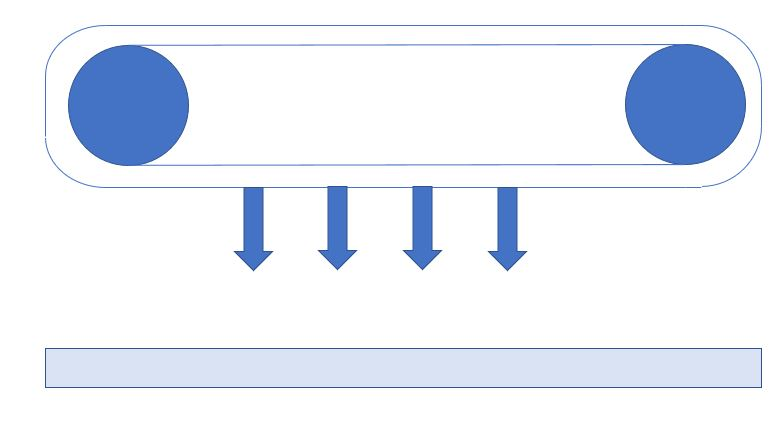
\includegraphics[width=\linewidth]{Bilder/Powerpoint/Foerderband}
      \caption{Foerderband}
      \label{Foerderband}
   \end{minipage}
   \hspace{.3\linewidth}% Abstand zwischen Bilder
   \begin{minipage}[hbt]{.2\linewidth} % [b] => Ausrichtung an \caption
      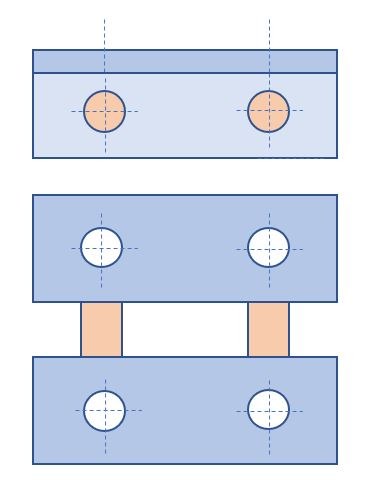
\includegraphics[width=\linewidth]{Bilder/Powerpoint/Kettenglied}
      \caption{Kettenglied}
	  \label{Kettenglied}      
      \end{minipage}
\end{figure}

\subsubsection{Walze}

Nach dem die Futterpackung in Bewegung ist, wird bei einer gewissen Position die Klemme entfernt und durch die Walze gepressen. Die Walze ist innen hohl und wird auf der Welle plaziert. Die eine auf der Antriebsseite und die andere auf einer eigengefertigten Welle. Beide Walzen werden durch eine Feder aneinander gepresst, nur so stark, damit die Halterung, an der die Packung festgemacht ist, durchkommt. Dennoch so stark damit sich die Packung entleert. Die Walze an der eigengefertigeten Welle wird mit zwei Aluplatten und einem Schanier in Stellung gehalten. Siehe Abbildungen: \ref{Walze}, \ref{Schanier}.

\begin{figure}[H]
   \begin{minipage}[hbt]{.4\linewidth} % [b] => Ausrichtung an \caption
      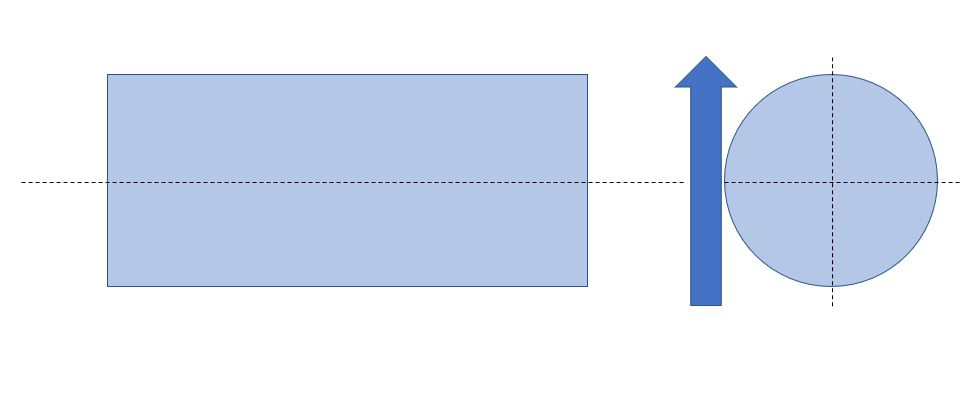
\includegraphics[width=\linewidth]{Bilder/Powerpoint/Walze}
      \caption{Walze}
      \label{Walze}
   \end{minipage}
   \hspace{.2\linewidth}% Abstand zwischen Bilder
   \begin{minipage}[hbt]{.4\linewidth} % [b] => Ausrichtung an \caption
      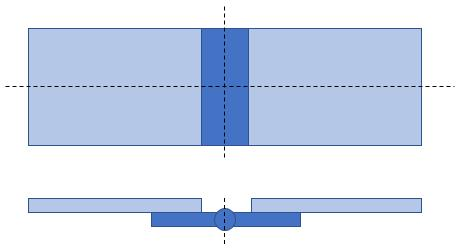
\includegraphics[width=\linewidth]{Bilder/Powerpoint/Schanier}
      \caption{Schanier}
	  \label{Schanier}      
      \end{minipage}
\end{figure}

\newpage
\subsubsection{Futterplatte}

\begin{wrapfigure}{r}{0.5\textwidth}
\vspace{-30pt}
  \begin{center}
    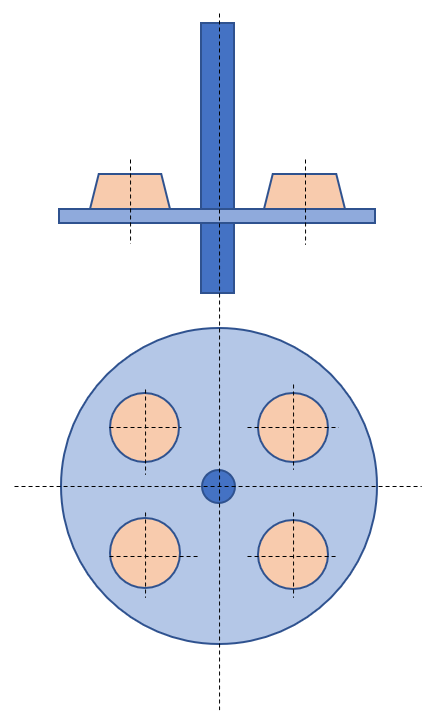
\includegraphics[width=0.32\textwidth]{Bilder/Powerpoint/Futterplatte}
  \end{center}
  \caption{Futterplatte}
  \label{Futterplatte}
  \vspace{-20pt}
\end{wrapfigure}


Nach dem Pressen wird das Futter in die Schüssel gequetscht bzw. es rinnt in die Schüssel. Die Platte hat eine gewisse Anzahl an Schüsseln, je nach Bedarf maximal fünf Schüsseln. Diese sind auf einer Platte plaziert, durch den Plattenmittelpunkt geht eine Welle die die Platte nach links und rechts drehen kann. Siehe Abbildung: \ref{Futterplatte}



\subsection{Variante 3}

In dieser Variante wurde überlegt, ob man das Futter nicht einfrieren kann, dieses danach aus der Gefriertruhe holt und erwärmt. Der Vorteil hierbei ist es können keine Schädlinge in das Futter gelange da es tiefgefroren ist und es kann die Portionsgröße eingestellt werden wieviel die Katze bekommt da der Benutzer die Menge an Futter selbst bestimmen kann.  Weiters müsste man nicht über das Schneide Problem nachdenken, da es eine knifflige Anglegenheit ist die Packung bei jeden Schnitt perfekt zu schneiden. Der große Nachteil ist der Platzbedarf und der hohe Energieverbrauch der Kühltruhe. Auch die Entnahme des Futters aus der Kühltruhe ist kein leichtes Unterfangen, da man entwerder viel mit Magnetzylinder arbeiten muss zur Verschiebung der Abdeckung oder ein Loch aus dem der Greifer das Futter entnimmt und dicht Halten muss, damit die Kühltruhe nicht zu warm wird, alles zerschmiltz und schlussendlich das Futter verdirbt. Hinzuzufügen ist auch noch das Katzen wenn es um Futter geht séhr wählerisch sind und somit wenn das Futter gefroren ist, hat man zu einem  Teil das Kontenzwasser des aufgetauten Futters und zum Anderen schmecht eingeforenes Essen anders, also nicht so wie es die Katze gewohnt ist.

\newpage
\section{Aufbauten und Tests}

In diesem Abschnitt der Diplomarbeit werden verschiedene Tests der obigen Varianten zu sehen sein. \\

\subsection{Fütterungsexperiment} 

In diesem Experiment wurde getestet wie lange es Dauert bis eine Packung nur mit Hilfe der Schwerkraft ausläuft. Der Beutel wurde nicht extra erwärmt und wird nur an den beiden unteren Ecken gehalten. Siehe Abbildungen: \ref{Halterung}, \ref{Fütterungs Anfang}, \ref{Fütterungs Mitte}

\begin{figure}[H]
   \begin{minipage}[hbt]{.4\linewidth} % [b] => Ausrichtung an \caption
      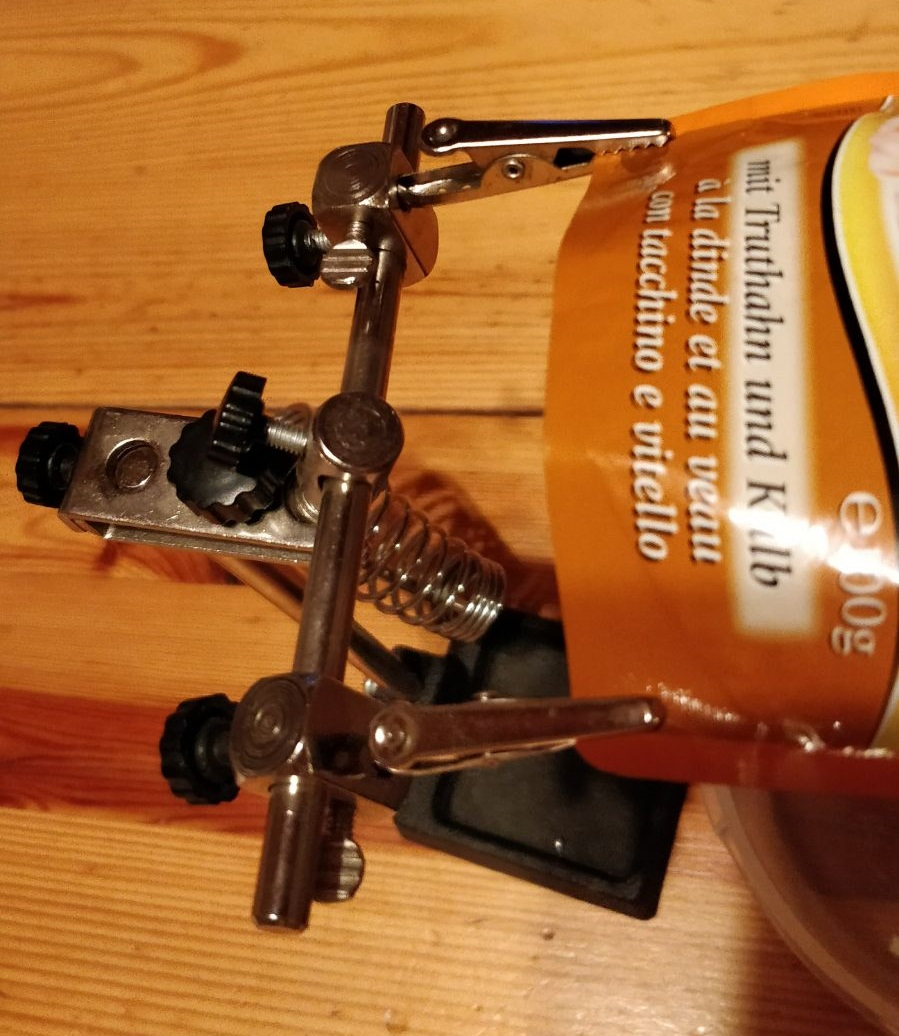
\includegraphics[width=\linewidth]{Bilder/Fuetterungsexperiment/Aufhaengung}
      \caption{Halterung}
      \label{Halterung}
   \end{minipage}
   \hspace{.2\linewidth}% Abstand zwischen Bilder
   \begin{minipage}[hbt]{.4\linewidth} % [b] => Ausrichtung an \caption
      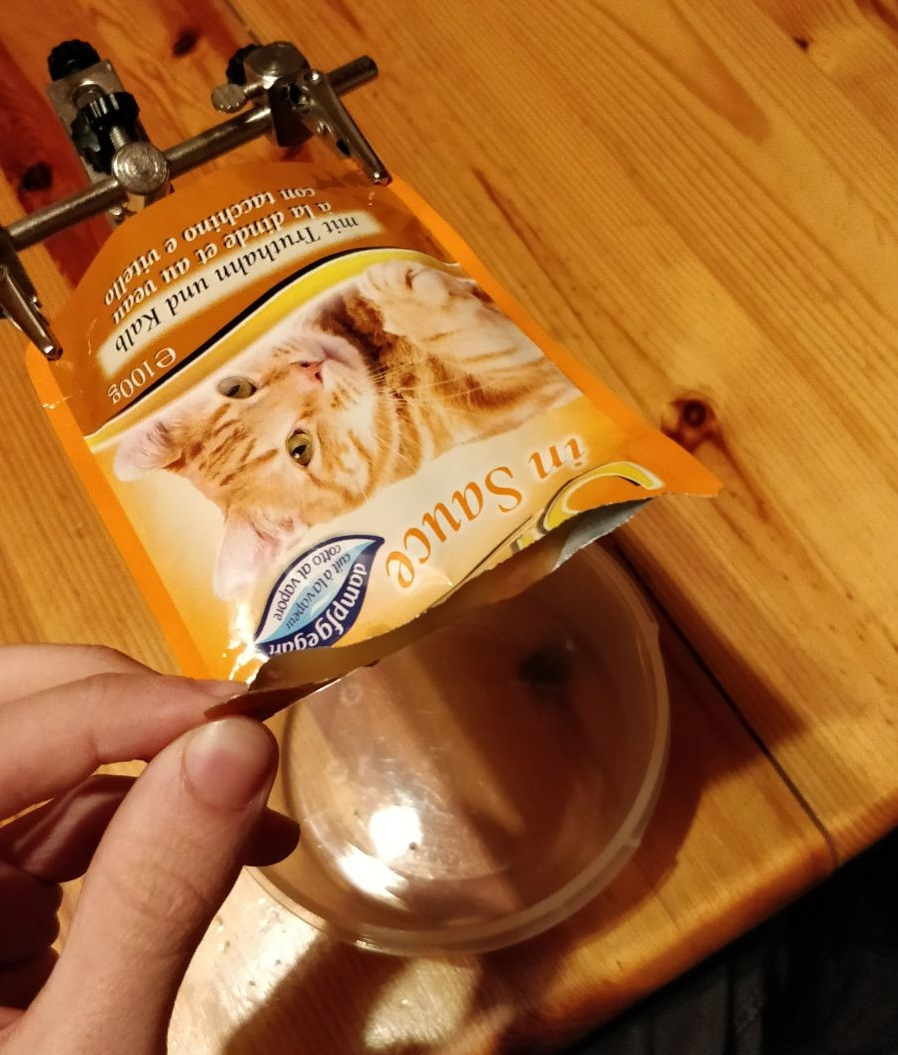
\includegraphics[width=\linewidth]{Bilder/Fuetterungsexperiment/Fuetterungs_Anfang}
      \caption{Fütterungs Anfang}
	  \label{Fütterungs Anfang}      
      \end{minipage}
\end{figure}


\begin{figure}[H]
   \begin{minipage}[hbt]{.3\linewidth} % [b] => Ausrichtung an \caption
      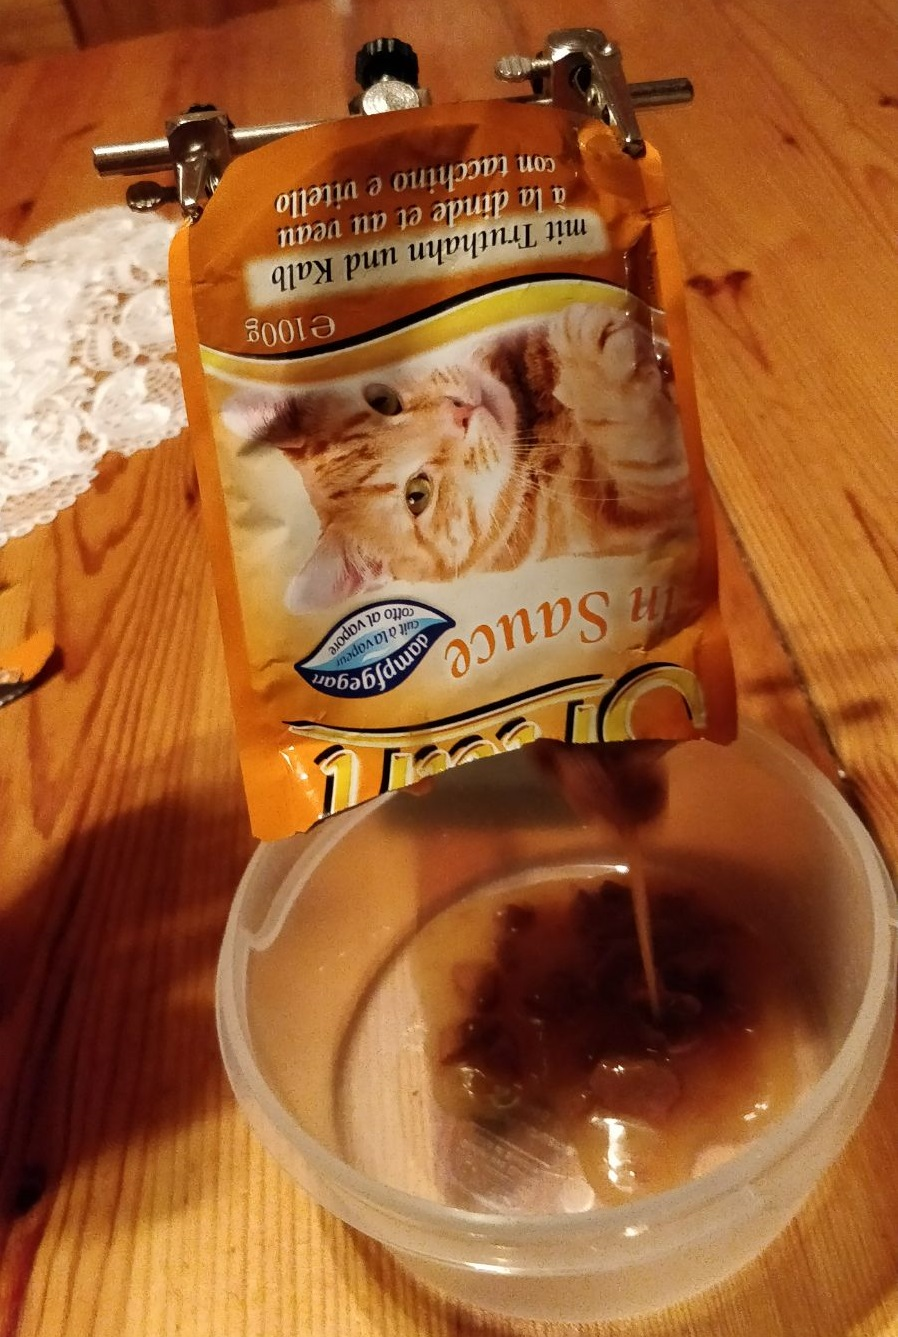
\includegraphics[width=\linewidth]{Bilder/Fuetterungsexperiment/Fuetterungs_Mitte}
      \caption{Fütterungs Mitte}
      \label{Fütterungs Mitte}
   \end{minipage}
   \hspace{.4\linewidth}% Abstand zwischen Bilder
   \begin{minipage}[hbt]{.3\linewidth} % [b] => Ausrichtung an \caption
     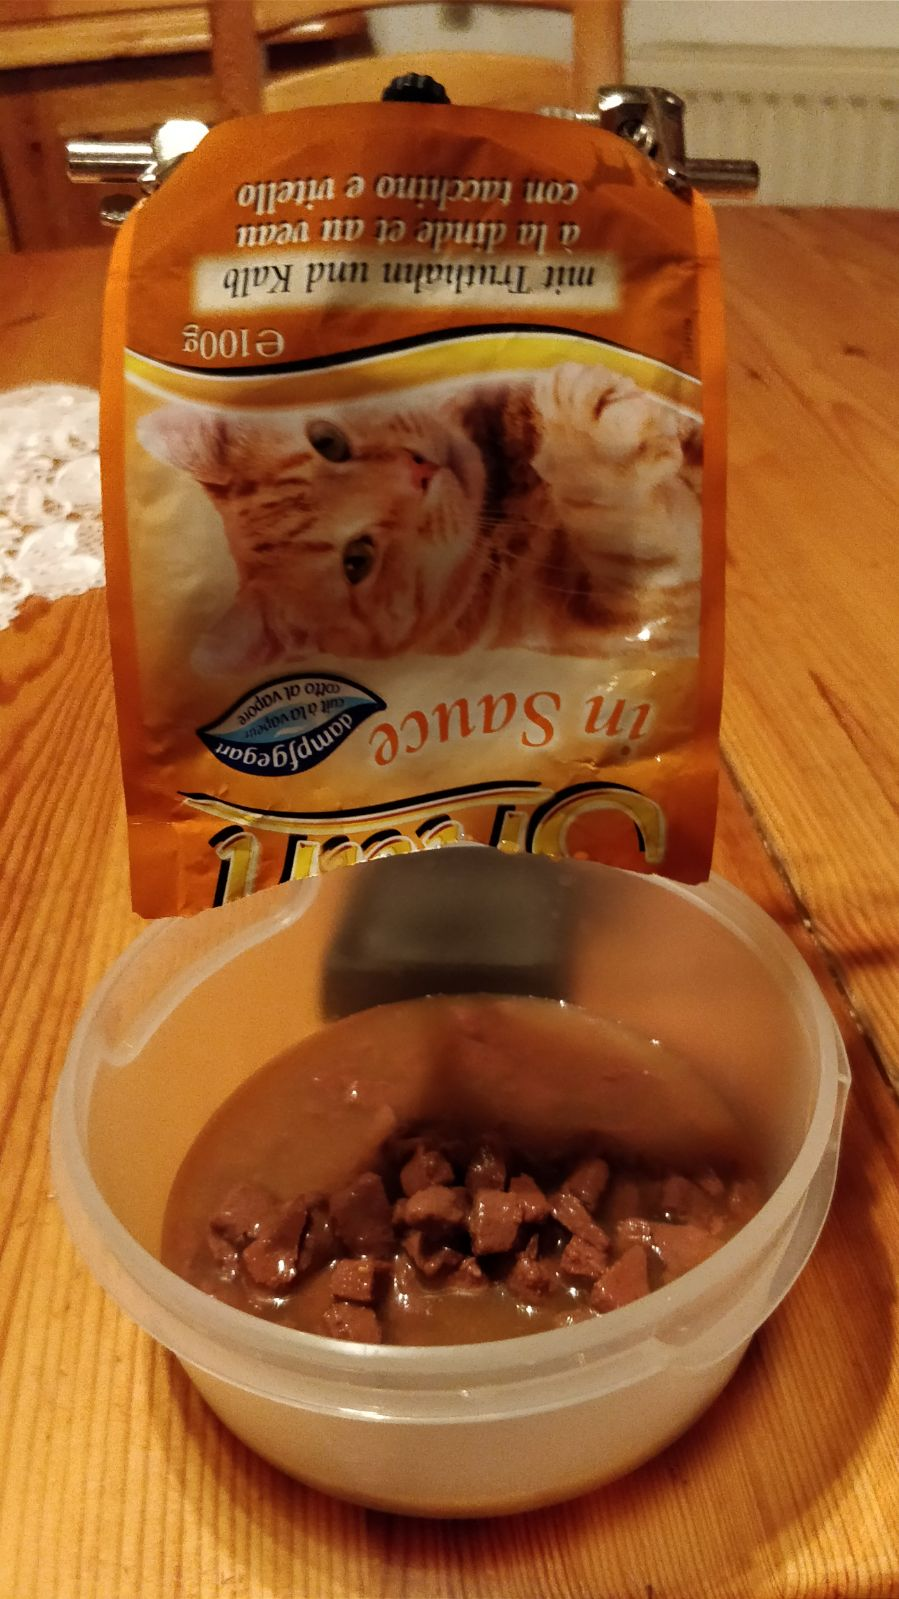
\includegraphics[width=\linewidth]{Bilder/Fuetterungsexperiment/Fuetterungs_Ende}  
      \caption{Fütterungs Ende}
     \label{Fütterungs_Ende}
   \end{minipage}
\end{figure}

In der Abbildung: \ref{Fütterungs_Ende} sieht man das nach 10 Minuten der Inhalte ganz in der Futterschüssel ist, dennoch Tropft es nach.
\newpage
\subsection{Schneideversuch 1.Art der 1.Variante}

Schnitt anhand einer praxischen Anwendung dargestellt. Der Beutel wird mithilfe einer Papierschneidemaschine geschnitten. Siehe Abbildungen: \ref{Einlegen}, \ref{Anfangsschnitt}, \ref{Endschnitt}

\begin{figure}[H]
   \begin{minipage}[hbt]{.3\linewidth} % [b] => Ausrichtung an \caption
      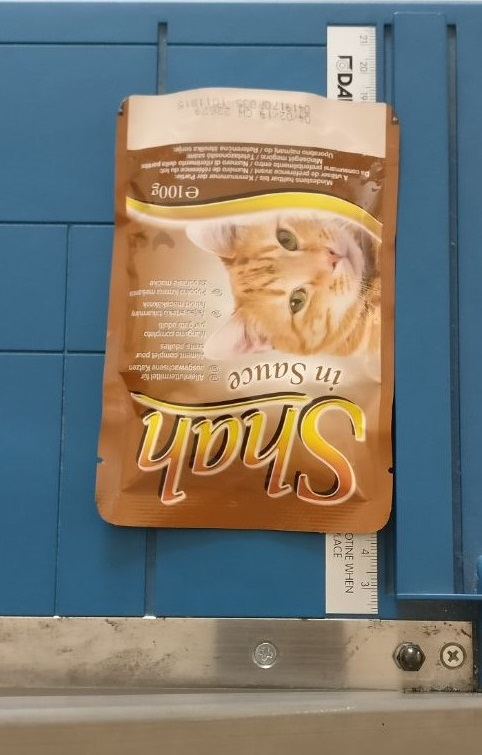
\includegraphics[width=\linewidth]{Bilder/Schneideversuch_1.Art/Einlegen}
      \caption{Einlegen}
      \label{Einlegen} 
   \end{minipage}
   \hspace{.2\linewidth}% Abstand zwischen Bilder
   \begin{minipage}[hbt]{.5\linewidth} % [b] => Ausrichtung an \caption
      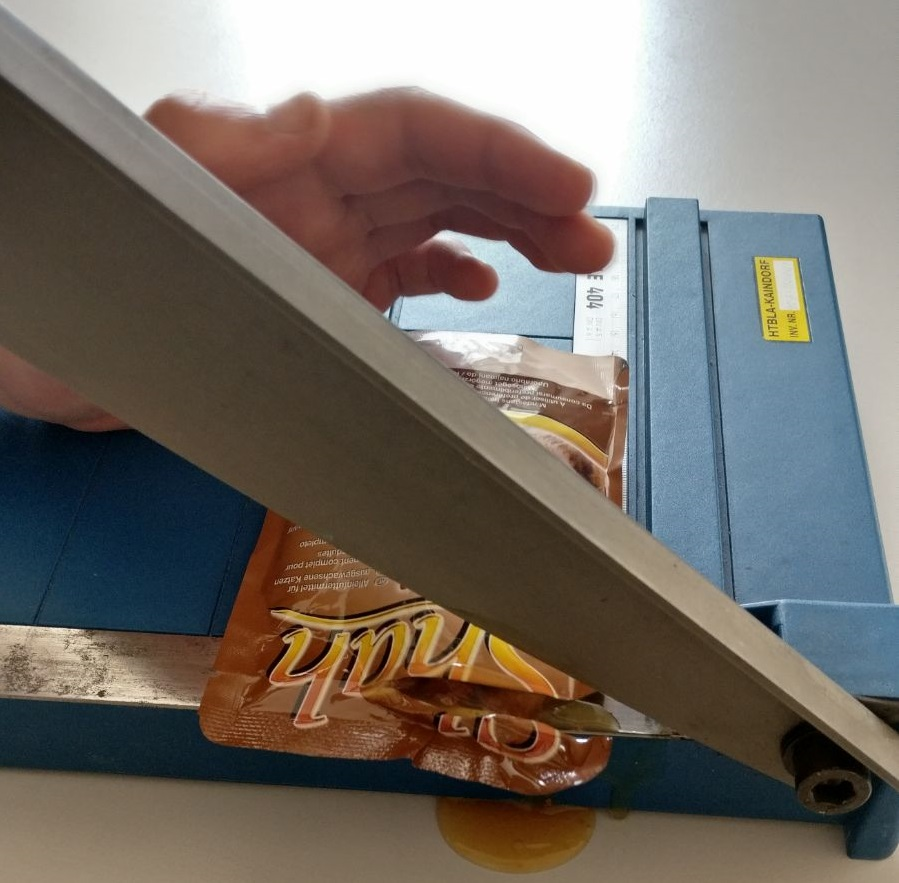
\includegraphics[width=\linewidth]{Bilder/Schneideversuch_1.Art/Anfangsschnitt}
      \caption{Anfangsschnitt}
      \label{Anfangsschnitt} 
   \end{minipage}
\end{figure}

\begin{figure}[H]
\begin{center}
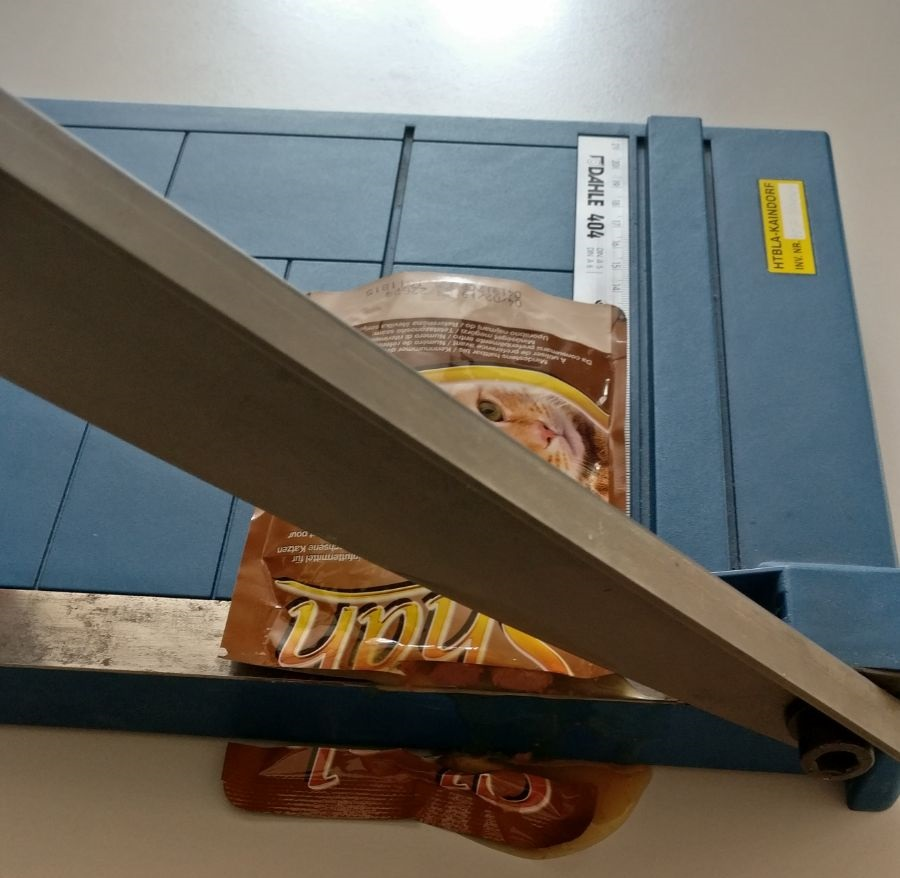
\includegraphics[width=7cm]{Bilder/Schneideversuch_1.Art/Endschnitt}
\caption{Endschnitt}
\label{Endschnitt} 
\end{center}
\end{figure}
\newpage
\subsection{Schneideversuch 2.Art der 1.Variante}

Mit einem Metallwerkzeug mit Wellenschliffartiger Kante wird der Futterbeutel entlang der Oberseite aufgeschnitten. Um die Packung vollständig geöffnet zu haben, mussten mehrere Schnitte verwendet werden. Siehe Abbildung: \ref{Schneidemittel}

\begin{figure}[H]
   \begin{minipage}[hbt]{.3\linewidth} % [b] => Ausrichtung an \caption
      \includegraphics[width=\linewidth]{Bilder/Schneideversuch_2.Art/Schneidemittel}
      \caption{Schneidemittel}
      \label{Schneidemittel} 
   \end{minipage}
   \hspace{.4\linewidth}% Abstand zwischen Bilder
   \begin{minipage}[hbt]{.3\linewidth} % [b] => Ausrichtung an \caption
      \includegraphics[width=\linewidth]{Bilder/Schneideversuch_2.Art/Anfangsschnitt}
      \caption{Anfangsschnitt 2.Art}
      \label{Nach 3 Schnitten}
   \end{minipage}
\end{figure}

In der Abbildung: \ref{Nach 3 Schnitten} erkennt man wie offen die Packung nach 3 Schnitten ist.

\begin{figure}[H]
   \begin{minipage}[hbt]{.4\linewidth} % [b] => Ausrichtung an \caption
      \includegraphics[width=\linewidth]{Bilder/Schneideversuch_2.Art/Mittelschnitt}
      \caption{Mittelschnitt 2.Art}
      \label{Nach 6 Schnitten}
   \end{minipage}
   \hspace{.2\linewidth}% Abstand zwischen Bilder
   \begin{minipage}[hbt]{.4\linewidth} % [b] => Ausrichtung an \caption
      \includegraphics[width=\linewidth]{Bilder/Schneideversuch_2.Art/Endschnitt}
      \caption{Endschnitt 2.Art}
      \label{Nach 9 Schnitten}
   \end{minipage}
\end{figure}
In der Abbildung: \ref{Nach 6 Schnitten} erkennt man wie offen die Packung nach 6 Schnitten ist.\\

In der Abbildung: \ref{Nach 9 Schnitten} wurde die Packung nach 9 Schnitten vollständig geöffnet.

\section{Vergleich der Varianten}
\subsection{Klemmen}
\subsubsection{Einfache Klemme}

\begin{wrapfigure}{r}{0.5\textwidth}
\vspace{-20pt}
  \begin{center}
    \includegraphics[width=0.32\textwidth]{Bilder/Powerpoint/Einfach_Klemme}
  \end{center}
  \caption{Einfache Klemme}
  \label{Einfache Klemme}
  \vspace{-30pt}
\end{wrapfigure}

Die einfach Klemme ist für gewöhnliche Verpackungen gut zu nutzen jedoch ist sie für unsere Variante nicht zu gebrauchen, dadurch Kunstoff nicht so stabil wie Metall ist drück sie die Packung an manchen Stellen zu wenig zusammen und an diesen Stellen kann Flüssigkeit austreten. Außerdem hält sie bei Zugbelastung nur wenig stand. Siehe Abbildung: \ref{Einfache Klemme}

\subsubsection{Hebel Klemme} 

\begin{wrapfigure}{r}{0.5\textwidth}
\vspace{-30pt}
  \begin{center}
    \includegraphics[width=0.32\textwidth]{Bilder/Powerpoint/Hebel_Klemme}
  \end{center}
  \caption{Hebel Klemme}
  \label{Hebel Klemme}
  \vspace{-65pt}
\end{wrapfigure}

Die Hebel Klemme ist für diese Diplomarbeit die bevorzugte Methode sie kann viel Druck auf die Packung ausüben sodass keine Flüssigkeit entrinnen kann. Außerdem lässt sich durch den Hebel mit wenig Kraft die Klemme öffnen. Weiters können die Klemmen auf einer Stange aufgesammelt werden und liegen nicht an unerwünschten Positionen an denen man nicht herankommt. Siehe Abbildung:    
 \ref{Hebel Klemme}
 \vspace{40pt}


\subsubsection{Gummiband Klemme}
 
\begin{wrapfigure}{r}{0.5\textwidth}
\vspace{-40pt}
  \begin{center}
    \includegraphics[width=0.30\textwidth]{Bilder/Powerpoint/Gummiband_Klemme}
  \end{center}
  \caption{Gummiband Klemme}
  \label{Gummiband Klemme}
  \vspace{-20pt}
\end{wrapfigure}

Die Gummiband Klemme hat eine starke Klemmkraft, dies Schützt vor dem Aufplatzen der Verpackung. Das Problem dieser Variante ist das das Gummiband spröder werden kann und irgendwann reißen, also ein hoher Verschleiß. Die Klemmen kann man auch nicht kontrolliert sammeln und somit sind sie schwerer zugänglich.

\subsection{Futterschüsseln}

\subsubsection{Drehfutterplatte}

\begin{wrapfigure}{r}{0.5\textwidth}
\vspace{-40pt}
  \begin{center}
    \includegraphics[width=0.25\textwidth]{Bilder/Powerpoint/Drehplatte}
  \end{center}
  \caption{Drehplatte}
  \label{Drehplatte}
  \vspace{-20pt}
\end{wrapfigure}

Die Drehplatte besteht aus fünf Schüsseln man kann pro Schüssel die Katze 2-mal am Tag füttern abends und morgens. Dadurch hat die Katze jeden Tag einen neue Schüssel und falls sie nicht frisst muss sie nicht Hunger leiden. Auf einer Welle wird eine Platte befestigt 
darin werden fünf Löcher geschnitten und die Schüssel hinein gelegt. Die Drehplatte wird mit einen Schneckengewinde in die gewünschten Position gebracht. Siehe Abbildung:  	
 \ref{Drehplatte} \vspace{+80pt}
 

\subsubsection{Futterplatte Zylinder}

\begin{wrapfigure}{}{0.5\textwidth}
\vspace{-50pt}
  \begin{center}
    \includegraphics[width=0.32\textwidth]{Bilder/Powerpoint/Platte_Zylinder}
  \end{center}
  \caption{Platte Zylinder}
  \label{Platte Zylinder}
  \vspace{-20pt}
\end{wrapfigure}

Die Futterplatte mit Zylinder ist die umständlichste Variante. Es ist eine viereckige Platte auf der Schienen für das schieben der Futterschüsseln platziert sind. Diese werden von Magnetzylindern angeschoben. Der Nachteil hierbei ist, man benötigt viele Bauteile und alle Zylinder müssen zugleich arbeiten um die Futterschüssel zur richtigen Position zu führen. Siehe Abbildung: \ref{Platte Zylinder} 


\newpage
\subsubsection{Platte mit einer Schüssel}

\begin{wrapfigure}{r}{0.5\textwidth}
\vspace{-40pt}
  \begin{center}
    \includegraphics[width=0.17\textwidth]{Bilder/Powerpoint/Einschuessel_platte}
  \end{center}
  \caption{Einschüsselplatte}
  \label{Schüssel Eins}
  \vspace{-20pt}
\end{wrapfigure}

Die Platte mit nur einer Schüssel ist leicht zu realisieren da sie nur wenige Bauteile benötigt. Das wäre zum Einem die Platte auf der die Futterschüssel mit einer Schiene darauf platziert ist. Sowohl als auch die zwei Magnetzylinder die die Futterschüssel in die Anfangs und Endposition bringt. Jedoch ein großer Nachteil weswegen diese Methode nicht in Frage kommt ist, wenn die Katze nach dem Füttern nicht frisst dann bleibt der Inhalt in der Schale und trocknet ein oder es kommt Ungeziefer hinein. Das hat zu Folge das die Schüssel jeden Tag befüllt wird und übergeht. Siehe Abbildung: \ref{Schüssel Eins} 



\subsection{Futtermagazine}

\subsubsection{Futtermagazin Horizontal}

\begin{wrapfigure}{r}{0.5\textwidth}
\vspace{-40pt}
  \begin{center}
    \includegraphics[width=0.30\textwidth]{Bilder/Powerpoint/Futtermagazin_horizontal}
  \end{center}
  \caption{Futtermagazin Horizontal}
  \label{Magazin Horizontal}
  \vspace{-10pt}
\end{wrapfigure} 

Das Futtermagazin Horizontal wäre für die erste Variante optimal. Da man den gewünschten Vorrat an Futterpackungen in die abgetrennten Räume platziert. Somit ist es einfach die gewünschte Position anzufahren und mit einen Greifer in die Schneideposition zu bringen. Der Aufbau ist wie ein Förderband, zwei Räder, ein Band mit oben platzierten Trennwänden und ein Motor der dieses Futtermagazin in Bewegung bringt. Zu beachten wäre wie die Futterpackungen ins Magazin eingelegt werden, nämlich mit der dünneren Fläche mit der Einkerbung die der Hersteller angegeben hat. Siehe Abbildung: \ref{Magazin Horizontal}
\newpage
\subsubsection{Futtermagazin Vertikal}

\begin{wrapfigure}{r}{0.5\textwidth}
\vspace{-40pt}
  \begin{center}
    \includegraphics[width=0.26\textwidth]{Bilder/Powerpoint/Futtermagazin_vertikal}
  \end{center}
  \caption{Futtermagazin Vertikal}
  \label{Magazin Vertikal}
  \vspace{-10pt}
\end{wrapfigure}

Das Futtermagazin Vertikal ist ein rechteckiges Gehäuse an denen 4 Magnetzylinder platziert werden. In dieser Box kommen die 10 Futterpackungen. Der Ablauf funktioniert in einer gewissen Reihenfolge. Zuerst öffnet sich der erste linke Magnetzylinder danach der gegenüberliegende zweite Magnetzylinder. Daraufhin gelangt die erste Futterpackung auf die unteren Zylinder. Nach diesem Schritt schließen sich die beiden Magnetzylinder wieder, damit die anderen Packungen nach den öffnen der unteren Magnetzylinder nicht durch die Maschine fallen. Daraufhin wenn der Fütterungsbefehl kommt öffnen sich die unteren Zylinder und die Packung gleitet über ein Blech zur Schnittfläche. Der große Nachteil dieser Methode ist das immer wieder Fehler auftreten können. Die Futterpackung kann falsch an der Schneidfläche ankommen bzw. sich an einem bestimmten Ort verkeilen. Siehe Abbildung: \ref{Magazin Vertikal}

\section{Konstruktion der Wahlvariante und Details}

\subsection{Drehplatte}
\subsection{Förderband}
\subsection{Walze}
\section{Berechnung und Dimensionierung}
\section{Simulation}
\section{Bedienung und Wartung}
\section{Selbstkritische Analyse und Ausblick}


\ihead{Julian Wolf}
\chapter{Elektronik und Mechanik}
\label{sec:elektronik-und-mechanik}

\section{Anforderung Elektronik Variante 1}
\subsection{Aktoren}
Die Aufgabe der Aktoren im elektrischen Teil besteht darin, ein Förderband und eine Drehplatte anzutreiben. Für beide Anwendungen werden Motoren mit einem hohen Drehmoment und einer niedrigen Drehzahl benötigt. Weiteres dürfen sich die Motoren nicht drehen, wenn sie nicht angesteuert werden.
Zur Positionierung, Befestigung und Durchführung anderer linearer Bewegungen werden Hubmagnete in Form von Zylindermagneten benötigt. Diese haben die Aufgabe Futterbeutel zu verschieben, zu positionieren, festzuhalten und einen Scherenhebel zum öffnen der Futterbeutel zu betätigen.  
\subsection{Sensoren}
Die Aufgabe der Sensoren im elektrischen Teil besteht darin, zu erkennen, ob ein Objekt vor ihnen steht. Dadurch kann überprüft werden, ob Futterschüsseln und Futterbeutel an der richtigen Stelle stehen.
\subsection{Ansteuerungen}
Die Aufgabe der Ansteuerung ist es, mithilfe eines Raspberrys und einem Arduino Nano, Motoren anzusteuern so wie Sensoren abzufragen. 
\newpage

\section{Anforderung Elektronik Variante 2}
\subsection{Aktoren}
Die Aufgabe der Aktoren im elektrischen Teil besteht darin, ein Förderband und eine Drehplatte anzutreiben. Für beide Anwendungen werden Motoren mit einem hohen Drehmoment und einer niedrigen Drehzahl benötigt. Zusätzlich dürfen sich die Motoren nicht drehen, wenn sie nicht angesteuert werden.
\subsection{Sensoren}
Die Aufgabe der Sensoren im elektrischen Teil besteht darin, zu erkennen, ob ein Objekt vor ihnen steht. Dadurch kann überprüft werden, ob Futterschüsseln und Futterbeutel an der richtigen Stelle stehen.
\subsection{Ansteuerungen}
Die Aufgabe der Ansteuerung ist es, mithilfe eines Raspberrys und einem Arduino Nano, Motoren anzusteuern so wie Sensoren abzufragen. \\

\section{Variante 1}
\subsection{Aktoren}
\subsubsection{Hubmagnete}
\begin{figure}[H] 
\begin{center}

\includegraphics[width=5cm]{Bilder/Bauteile/Hubmagnet}
\caption{Hubmagnet}
\label{Hubmagnet}

\end{center}
\end{figure}
Zylinderhubmagnete bestehen aus einem zylindrischen Dauermagnetkern. Umgeben ist dieser Magnetkern von einer Spule und einem Gehäuse, welches als Schutz vor Festkörpern dient. Wird an die Spule eine Spannung angelegt, fließt ein Strom durch die Spule und erzeugt ein Magnetfeld welches den Magnetkern anzieht oder abstößt. Durch eine gezielte Übersteuerung des Magnetzylinders kann die Kraft des Magnetfeldes kurzzeitig verstärkt werden, jedoch verhindert die erhöhte Hitzeentwicklung einen dauerhaften Betrieb im übersteuerten Zustand. Der übersteuerte Zustand wird mit einer geringeren relativen Einschaltdauer gegenüber der Zykluszeit bewirkt. \\Der Strom, der durch die Spule fließt, kann sich durch die kurze Einschaltdauer nicht einpendeln was der Spule erlaubt mit einem durchschnittlich höheren Strom betrieben zu werden, das wiederum zu einem stärkeren Magnetfeld und somit zu einer stärkeren Kraft führt. Die genauen Werte der Kraft zur relativen Einschaltdauer lassen sich dem Datenblatt jedes einzelnen Hubmagneten entnehmen. Ein Vorteil von Hubmagneten ist es, dass sie in allen möglichen Formen, Hublängen, Hubkräften und Wechsel- oder Gleichspannungsbereichen verfügbar sind. Hubmagnete können mit drei verschiedenen Hubzuständen erworben werden. Monostabile Hubmagnete halten sich mithilfe einer Feder bei stromlosem Zustand immer an der Anfangs oder Endposition. Bistabile Hubmagnete verweilen im stromlosem Zustand an ihrer aktuellen Position, also entweder im eingefahrenen oder ausgefahrenen Zustand. Tristabile Hubmagnete bleiben, wie bistabile Hubmagnete, stromlos an ihrer aktuellen Position. Jedoch kann diese Hubmagnetart auch an einer vorgegebenen Mittelposition verweilen.

\subsubsection{Motoren}
Nach einigen Problemen und Variantenänderungen in der Mechanik, wurde die Motorenauswahl erst in Variante 2 vorgenommen, da die Auswahl für Variante 1 sinnfrei wäre.

\subsection{Sensoren}
\begin{figure}[H] 
\begin{center}

\includegraphics[width=5cm]{Bilder/Bauteile/Sensor}
\caption{Sensor}
\label{Sensor}

\end{center}
\end{figure}
Die Auswahl des Sensors für unsere Anwendung wurde durch folgende Kriterien beeinflusst: Befestigungsmöglichkeiten, Preis und zusätzlich benötigte Ansteuerungen.
Kapazitive und induktive Näherungsschalter lassen sich einfach befestigen, sind jedoch in der Anschaffung teuer. Die Reichweite der Sensoren ist nicht sehr groß, was aber für unsere Anwendung nicht relevant ist. Für diese Arten von Sensoren werden zusätzliche Ansteuerungen benötigt. Diese Ansteuerungen sind meistens etwas teuerer und benötigen zur Kommunikation mit einem Raspberry eine Schnittstelle.
Aus diesen Gründen haben wir uns in diesem Anwendungsbereich für einen optischen Näherungsschalter entschieden. Dieser beinhaltet ein fertiges Modul bestehend aus einer Infrarot LED und einem Infrarot Fototransistor. Dieses Modul ist preiswert und leicht zu befestigen. Dadurch, dass unsere Anwendung keine genaue Abstandsmessung erfordert, wird keine zusätzliche Ansteuerung benötigt. Zur Stromversorgung reichen 5V Gleichspannung mit einem laut Datenblatt berechneten Vorwiderstand. Die Auswertung erfolgt durch einen digitalen Input-Pin des Raspberrys. Sobald sich eine Reflektorfläche vor dem Sensor bewegt, wird der Fototransistor niederohmig und ermöglicht einen Stromfluss. Dadurch liegt eine Spannung von 3,3V am Input-Pin an und wird vom Raspberry als HIGH-Zustand angesehen. Wenn die Reflektorfläche vom Modul nicht mehr erfasst wird, sperrt der Fototransistor, der Stromfluss wird unterbunden und am Input-Pin liegen nur mehr 0V an, was als LOW-Zustand angesehen wird. \\

Kennlinie des Sensors:

\begin{figure}[H]
  \begin{minipage}[hbt]{0.45\textwidth}
    \includegraphics[width=0.9\textwidth]{Bilder/Kennlinien/Sens_Vf_If}
 	\caption{Diodenspannung zu \\Diodenstrom}
  	\label{Sens_vf_if}
  \end{minipage}
\hspace{.03\linewidth}
  \begin{minipage}[hbt]{0.45\textwidth}
    \includegraphics[width=0.9\textwidth]{Bilder/Kennlinien/Sens_op_If}
  	\caption{Optische Übertragungs-\\stärke zu Diodenstrom}
  	\label{Sens_op_if}
  \end{minipage}
\end{figure}

\subsection{Ansteuerungen}
Da Variante 1 nur kurze Zeit verfolgt wurde, wurden genaue Ansteuerungen für Motoren und Hubmagnete nicht herausgesucht. Der Sensor benötigt keine zusätzliche Ansteuerung.
\newpage
\section{Variante 2}
\subsection{Aktoren}
\subsubsection{Hubmagnete}
Für die zweite Variante werden keine Hubmagnete benötigt.

\subsubsection{Motoren}
\begin{figure}[H] 
\begin{center}

\includegraphics[width=8cm]{Bilder/Bauteile/Motor}
\caption{Motor}
\label{Motor}

\end{center}
\end{figure}
Die Motoren wurden mithilfe folgender Kriterien ausgesucht: Preis, Drehzahl, Kraft, stromloses Verhalten und Spannung.
Wir haben uns  darauf festgelegt nur mit sicherer niedriger Gleichspannung zu arbeiten. Daher kommen nur Motoren mit einem Spannungsbereich von 0-24V in Frage. Aus diesem Grund werden die Auswahl eines Asynchronmotors ausgeschlossen. Die Anwendung fordert, dass sich die Motoren im stromlosem Zustand nicht bewegen lassen. Dadurch können folgende Motorarten ausgeschlossen werden: Synchronmotoren, reine Gleichstrommotoren, Schrittmotoren und Servomotoren, falls diese Motoren nicht über eine aktive Bremse verfügen. Ideal für unsere Anwendungen sind Gleichstrom-Schneckengetriebe-Motoren. Diese Motoren lassen sich aufgrund des mechanischen Aufbaus im stromlosem Zustand nicht drehen. Sie verfügen meistens auch über ein Getriebe, welches eine Übersetzung in eine niedrigere Drehzahl zur Folge hat. Gleichzeitig wird mit diesem Getriebe auch das Drehmoment erhöht, wodurch der Motor eine höhere Kraft aufbringen kann. Da Schneckengetriebemotoren in der Automobil Industrie als Scheibenwischermotoren verwendet werden, sind diese sehr preisgünstig zu erwerben.

\subsubsection{Lüfter}
\begin{figure}[H] 
\begin{center}

\includegraphics[width=5cm]{Bilder/Bauteile/Luefter}
\caption{Lüfter}
\label{Luefter}

\end{center}
\end{figure}
Zur Kühlung des Raspberrys, findet ein externer 12V-Lüfter Verwendung, welcher einen Luftstrom um den Raspberry und den \ac{uC}ontroller erzeugt.
\subsection{Sensoren}
Der ausgewählte optische Sensor wurde in Variante 1 bereits beschrieben. Für genauere Informationen lesen Sie bitte in Punkt 4.3.2 nach.
Es werden zwei dieser Sensoren zur Positionierung verwendet. Der Sensor muss nur erkennen, ob sich eine Reflektorfläche vor ihm befindet. Bei der Futterschüsseldrehplatte wird am Rand der Scheibe, an der Position jeder Futterschüssel ein Reflektorstreifen verwendet. Dadurch kann mit der Software gezählt und erkannt werden, welche Futterschüssel sich aktuell vor dem Sensor befindet. Im Futterbeutelmagazin wird der Sensor dazu verwendet, um erkennen zu können, ob ein Futterbeutel für die Fütterung verfügbar ist. Wird vom Sensor, nach Drehen des Motors, kein weiterer Futterbeutel erkannt, wird von der Software, falls nötig, ein Fehler ausgegeben und der Benutzer informiert. Der Reflektorstreifen wird auf der Verschlussklemme jedes Futterbeutels befestigt.
\subsection{Ansteuerung}
Der Gesamtschaltplan wurde in ProfiCad realisiert. Der Schaltplan beinhaltet die Ansteuerung der Motoren und Sensoren, sowie die Visualisierung der Verkabelung der einzelnen Elemente.
Für ein einfacheres Verständnis wird der Gesamtschaltplan in kleinere Elemente aufgeteilt und in Unterpunkten beschrieben.
\newpage
\subsubsection{Motoransteuerung Variante 1}
Der Gleichstrom Schneckengetriebemotor in unserer Anwendung kann in beide Richtungen betrieben werden, je nach Polarität der Anschlüsse. Um eine softwaretechnisch einfache Ansteuerung ermöglichen zu können, wird oft eine H-Brücke zur Ansteuerung der Motoren verwendet. Diese H-Brücke besteht aus vier Transistoren. Für Motoren mit höheren Stromanforderungen werden MOSFET-Transistoren verwendet. Die Schaltung besteht aus zwei P-Kanal MOSFET T1, T3 und aus zwei N-Kanal MOSFET T2, T4. Die Schaltung laut Abbildung \ref{HBridge}, wurde aus dem Web\footfullcite{HBridge} entnommen und abgeändert. Dabei wurden die Bauteilwerte der MOSFETs und Teile der Schaltung übernommen. Der Raspberry steuert über Optokoppler die MOSFETs. Dabei wird über eine entsprechende Vorschaltung entweder das Gate vom MOSFET auf Ground- oder 12V-Potenzial gezogen. Zur Veranschaulichung wurden in Abbildung \ref{HBridge} die Raspberry Pins mit einer Klemme ersetzt, wobei die Klemme 1, T1, Klemme 2, T2, Klemme 3, T3 und Klemme 4, T4 steuert. 

Es gibt bei dieser Ansteuerungsart folgende erwünschte Zustände der Klemmen: \\
\begin{table}[htb]
\centering
\begin{tabular}{|c|c|c|c|c|c|} \hline
Klemme & Uhrzeigersinn & gegen Uhrzeigersinn & Auslaufen & Bremsen & Bremsen \\ \hline
1 & HIGH & LOW & LOW & HIGH & LOW  \\ \hline
2 & LOW & HIGH & LOW & LOW & HIGH \\ \hline
3 & LOW & HIGH & LOW & HIGH & LOW \\ \hline
4 & HIGH & LOW & LOW & LOW & HIGH \\ \hline
\end{tabular}
\caption{H-Brückenzustände}
\label{HBridge states}
\end{table}

Jede unterschiedliche Beschaltungsart als die oben angeführten, würde zu einem Kurzschluss führen und muss softwaretechnisch verhindert werden. \\


Kennlinie der Transistoren:

\begin{figure}[H]
  \begin{minipage}[hbt]{0.45\textwidth}
    \includegraphics[width=0.9\textwidth]{Bilder/Kennlinien/P_Kanal}
 	\caption{P-Kanal}
  	\label{Pchannel}
  \end{minipage}
\hspace{.03\linewidth}
  \begin{minipage}[hbt]{0.45\textwidth}
    \includegraphics[width=0.9\textwidth]{Bilder/Kennlinien/N_Kanal}
  	\caption{N-Kanal}
  	\label{Nchannel}
  \end{minipage}
\end{figure}


\begin{figure}[H] 
\begin{center}

\includegraphics[width=15cm]{Bilder/Schaltplan/Schaltplan_HBridge}
\caption{H-Bridge}
\label{HBridge}

\end{center}
\end{figure}

Dieser Schaltplan dient nur als Beispiel-Schaltung und wurde aufgrund der Motoransteuerung Variante 2, nicht mehr weiter verfolgt. Um die Schaltung wirklich benutzen zu können, müsste eine Sicherung gegen einen Kurzschluss eingebaut werden. Für unsere Anwendung müsste eine Drehzahlregelung der Motoren Verwendung finden.
\newpage
\subsubsection{Motoransteuerung Variante 2}
\begin{figure}[H] 
\begin{center}

\includegraphics[width=6.5cm]{Bilder/Bauteile/Motorsteuerung}
\caption{Motorsteuerung}
\label{Motoransteuerung}

\end{center}
\end{figure}
Aus sicherheits- und kostentechnischen Gründen, wurde von einer manuell gesteuerten H-Brücke auf ein fertiges Motorsteuerungsmodul umgestiegen. Der Vorteil dieser Ansteuerung besteht darin, dass ein Kurzschluss der H-Brücke hardwaretechnisch ausgeschlossen werden kann und damit nicht von der Software abgesichert werden muss. Das Motormodul verfügt außerdem über eine interne Strommessung für jeden der zwei unterstützten Motoren. Diese Messung kann bei Bedarf abgefragt werden. Für unsere Anwendung ist dies jedoch nicht erforderlich. Der Motortreiber unterstützt zwei Motoren, welche mit bis zu 30 Ampere bei 16V betrieben werden können, bevor der IC überhitzt oder andere Bauteile zerstört werden. Die Ansteuerung jedes Motors erfolgt über ein digitales Signal. Motor Nr.1 kann über den Pin AI0 aktiviert (enabled) werden. Dies dient zur Sicherung, dass der Motor nicht aus Versehen betätigt werden kann, solange der AI0 Pin nicht auf HIGH ist. Der enable Pin für Motor Nr.2 ist AI1. Um Motor Nr.1 im Uhrzeigersinn drehen zu lassen, muss der Pin D7 mit einem HIGH Signal und der Pin D8 mit einem LOW Signal angesteuert werden. Um Motor Nr.2 gegen den Uhrzeigersinn drehen zu lassen, muss der Pin D8 mit einem HIGH Signal und der Pin D7 mit einem LOW Signal angesteuert werden. Um den Motor Nr.1 bremsen zu können, muss Pin D8 und D7 mit entweder einem HIGH oder einem LOW Signal angesteuert werden. Für Motor Nr.2 ist die Funktionsweise gleich, jedoch muss der Pin D7 mit Pin D4 und Pin D8 mit Pin D9 ersetzt werden. Die externe Stromversorgung für den IC von 5V erfolgt über den VCC Pin. Die externe Stromversorgung für die Motoren erfolgt über den PWR Pin. Zusätzlich muss der GND Pin noch mit einem der beiden Ground Anschlüsse der externen Stromversorgungen verbunden werden. Motor Nr.1 wird über die Outputs A1 und B1 versorgt. Motor Nr.2 wird über die Outputs A2 und B2 versorgt. Beim Anschluss der Motoren muss auf die Polung geachtet und gegebenenfalls getestet werden, ob sich die Motoren auch wirklich beim Ansteuern der D7 oder D4 Pins im Uhrzeigersinn drehen und nicht gegen den Uhrzeigersinn. Falls beim Motor gekennzeichnet, sollte der Pluspol des Motors mit dem A1 beziehungsweise dem A2 Pin verbunden werden. Der Motortreiber verfügt auch über eine interne Drehzahlregelung, welche extra für beide Motoren über zwei \ac{PWM} Input Pins gesteuert werden kann. Die Drehzahl kann über den Duty Cycle des \ac{PWM} Signals geregelt werden.
\subsubsection{PWM-Signal-erzeugung für Motoransteuerung}
\begin{figure}[H] 
\begin{center}

\includegraphics[width=12cm]{Bilder/PWM/Duty_Cycle}
\caption{PWM-Signal}
\label{PWM_Signal}

\end{center}
\end{figure}
Ein \ac{PWM} Signal ist ein periodisches Rechteck-Signal. Eine Periode wird als Duty Cycle bezeichnet. Dieser Duty Cycle enthält eine Prozentangabe, welche aussagt, wie viel Prozent des Duty Cycles HIGH und wie viel Prozent LOW sind. Ein Signal mit einem Duty Cycle von 100\% sagt aus, dass eine Periodendauer zu 100\% aus einem HIGH Signal und zu 0\% aus einem LOW Signal besteht. Ein Duty Cycle von 25\% sagt aus, dass eine Periode zu 25\% aus einem HIGH Signal und zu 75\% aus einem LOW Signal besteht. Das \ac{PWM} Signal kann von manchen ICs intern aufgenommen und der Duty Cycle ausgemessen werden. Dabei muss jedoch beachtet werden, dass die Frequenz des \ac{PWM} Signals nicht die maximale Schaltfrequenz des ICs übersteigt. In den meisten Fällen wird diese Frequenz, wie bei unserem Motortreiber, im Datenblatt angegeben. Das \ac{PWM} kann entweder über eigene ICs mit \ac{PWM} Generatoren oder \ac{uC}s mit internen \ac{PWM} Generatoren erzeugt werden. Das System muss nur über eine Echtzeitfähigkeit besitzen, damit der Duty Cycle keine Takte beim Zählen überspringen und nicht die Frequenz fehlerhaft werden kann. 
Unser \ac{PWM} Generator wurde mithilfe eines Arduino Nanos realisiert. Mithilfe des \ac{uC} Atmega328P wird der interne Zähler (Timer 2) dazu verwendet, einen Output Pin in den richtigen Abständen zu toggeln (von HIGH auf LOW oder umgekehrt schalten) um ein \ac{PWM} Signal zu erzeugen.


\begin{itemize}
\item verwendete Register:
\begin{itemize}
\item TCCR2A: Im TCCR2A Register wird festgelegt, in welchem Modus der Timer laufen soll und was mit den Pins OC2A und OC2B passieren soll, wenn der der aktuelle Timer-Wert mit einem der beiden Output Compare Register übereinstimmt. Die Bits COM2A1 und COM2A0 setzen im Fast-\ac{PWM} Modus fest, ob der OC2A Pin nicht beeinflusst wird und nicht verbunden ist, vom WGM22 Bit abhängig ist oder bei einem Compare Match, also wenn das Output Compare Register OCR2A mit dem aktuellen Timer Wert übereinstimmt, der OC2A Pin gesetzt und beim Reset des Timers resetet wird (non-inverting Mode), oder bei einem Compare Match der OC2A Pin resetet und beim Reset des Timers gesetzt wird (inverting Mode). \\ Die selbe Funktion haben die Bits COM2B1 und COM2B0, nur dass der Pin OC2B verändert und mit dem Compare Registe OCR2B verglichen wird. \\
Die Bits WGM21 und WGM20 setzen den Modus des Signalgenerators, die vom Timer unterstützt werden. Es gibt grundsätzlich drei Modi, in denen der Signalgenerator laufen kann: CTC, Fast \ac{PWM}, \ac{PWM} Phase Correct. \\
\begin{itemize}
\item Im CTC Modus kann der TOP Wert, zu dem der Counter zählt, immer bei jedem vollständigen Zählvorgang geändert werden. Der Zähler zählt in Form eines Sägezahn Signals und toggled den Pin immer, wenn der Top Wert erreicht wird.\\
\item Im Fast \ac{PWM} Modus zählt der Zähler in Form eines Sägezahnsignals und es wird bei jedem Zählschritt überprüft, ob der aktuelle Wert des Zählers mit dem Output Compare Register übereinstimmt. Was passiert, wenn die Werte übereinstimmen, wird in den COM2xx Bits festgelegt. Die Frequenz des Ausgangssignals am Pin kann nur über einen Prescaler verändert werden. Das bedeutet, dass die Frequenz nur sieben Frequenzen mit dem internen Timer annehmen kann. Das OCR2x Register kann während des Betriebes geändert werden. Damit kann der Duty Cycle während des Betriebes geändert werden. \\
\item Der \ac{PWM} Phase Correct Modus, lässt den Zähler von Bottom zu Top und wieder zu Bottom zählen. Das bewirkt, dass er Zähler in Form eines Dreiecksignals zählt. Somit ist das Ausgangs \ac{PWM} Signal immer symmetrisch um den BOTTOM und TOP Wert des Zählers. Daher bleibt das Signal immer Phasen-korrekt. Der Nachteil dieses Modus ist, dass er nur die halbe Frequenz des Fast \ac{PWM} Modus erreichen kann. Der \ac{PWM} Phase Correct Modus kann auch nur sieben Frequenzen annehmen.\\
\end{itemize} 
\item TCCR2B: Im TCCR2B Register wird für unsere Anwendung der Prescaler festgelegt, um die Frequenz des \ac{PWM}-Signales einzustellen. Dazu werden die Bits 0 bis 2 verwendet. Das sind die Bits CS20, CS21 und CS22. Die Bits FOC2A, FOC2B und WGM22 werden in unserer Anwendung nicht benötigt und können ignoriert werden. \\
\item OCR2A: Das Register OCR2A ist das Output Compare Match Register für den OC2A Pin. Das Register kann einen Wert zwischen 0 und 255 haben, wobei im Fast \ac{PWM} Modus 0 einem Duty Cycle von 0\% und 255 einem Duty Cycle von 100\% entspricht.\\
\item OCR2B: Das Register OCR2B ist das Output Compare Match Register für den OC2B Pin. Das Register kann einen Wert zwischen 0 und 255 haben, wobei im Fast \ac{PWM} Modus 0 einem Duty Cycle von 0\% und 255 einem Duty Cycle von 100\% entspricht.\\
\item DDRD: Im Register DDRD können I/O Pins als Output Pins gesetzt werden. Es muss nur das Bit des entsprechenden Pins gesetzt werden.\\
\item DDRB: Im Register DDRB können I/O Pins als Output Pins gesetzt werden. Es muss nur das Bit des entsprechenden Pins gesetzt werden.\\
\end{itemize}
\item Frequenz berechnen:\\
Die maximal Frequenz des \ac{PWM}-Signals für die Motoransteuerung beträgt 20kHz. Das bedeutet, dass man einen Frequenzwert so nahe wie möglich, aber unter der maximalen Frequenz wählen soll.\\
Berechnen lässt sich die Frequenz des \ac{PWM}-Signals mit folgender Formel:
\begin{align*}
f_{OC2xPWM}=\frac{f_{clk\_I/O}}{N*256} \\
\end{align*} 
f$_{OC2xPWM}$ ist die Frequenz, die das \ac{PWM}-Signal haben wird.\\
f$_{clk_I/O}$ ist die Taktfrequenz des Atmega328P, also 16MHz. \\
N ist der Wert des Prescalers, welcher im TCCR2B Register festgelegt wird. \\

\textbf{Frequenz Berechnung:}\\
$f_{OC2xPWM}$=$\frac{f_{clk\_I/O}}{N*256}$ = $\frac{16000000}{8 \cdot 256}$ = $\underline{7812,5Hz}$
\item Programm für Atmega328P: \\
\begin{lstlisting}[caption=$\mu$C-Programm,style=C]
void app_main (void)
{
  DDRD = (1<<PD3);
  DDRB = (1<<PB3);
  TCCR2A = (1<<COM2A1) | (1<<COM2B1) | (1<<WGM21) | (1<<WGM20);
  TCCR2B = (1<<CS21);
  OCR2A = 0x5f;
  OCR2B = 0x5f;
  
}
\end{lstlisting}
\newpage
\begin{itemize}
\item DDRD: Im DDRD Register wird der PD3 Pin auf Output geschaltet.
\item DDRB: Im DDRB Register wird der PB3 Pin auf Output geschaltet.
\item TCCR2A: Im TCCR2A Register wird der Non-Inverting Fast-\ac{PWM} Modus eingestellt für OC2A und OC2B. 
\item TCCR2B: Im TCCR2B Register wird der Prescaler festgelegt. 
\item OCR2A: Im OCR2A Register wird der Duty Cycle festgelegt. 0 entspricht 0\% und 255 entspricht 100\% 
\item OCR2B: Im OCR2B Register wird der Duty Cycle festgelegt. 0 entspricht 0\% und 255 entspricht 100\% 
\end{itemize}
\end{itemize}

Ein Signal, dass nach dem oben angeführten Programm generiert wird, sieht wie in Abbildung \ref{PWM} aus.
\begin{figure}[H] 
\begin{center}

\includegraphics[width=13cm]{Bilder/PWM/PWM}
\caption{PWM-Signal}
\label{PWM}

\end{center}
\end{figure}
\newpage
\subsubsection{Optokoppler}

Die Optokoppler in unserer Anwendung werden zur Potenzialerhöhung oder Potenzialverminderung von 3,3V auf 5V oder umgekehrt verwendet. Durch eine LED und einen Phototransistor werden die Schaltkreise getrennt. Wenn an der LED eine Spannung anliegt, beginnt sie zu leuchten und erhöht damit die Leitfähigkeit des Phototransistors. Dadurch ermöglicht ein Stromfluss der LED-Schaltung einen Stromfluss in der Phototransistor-Schaltung.

Kennlinie des Optokopplers:

\begin{figure}[H]
  \begin{minipage}[hbt]{0.45\textwidth}
    \includegraphics[width=0.9\textwidth]{Bilder/Kennlinien/Opto_Vf_If}
 	\caption{Diodenstrom zu \\Diodenspannung}
  	\label{Opto_Vf_If}
  \end{minipage}
\hspace{.03\linewidth}
  \begin{minipage}[hbt]{0.45\textwidth}
    \includegraphics[width=0.9\textwidth]{Bilder/Kennlinien/Opto_Vce_Ic}
  	\caption{Transistorstrom zu \\Transistorspannung}
  	\label{Opto_Vce_Ic}
  \end{minipage}
\end{figure}
\subsubsection{Gesamtschaltplan}
\begin{figure}[H]
\begin{minipage}[t]{6cm}
\vspace{0pt}
\centering
\includegraphics[width=8cm]{Bilder/Schaltplan/Blockschaltbild}
\caption{Blockschaltbild}
\label{Blockschaltbild}
\end{minipage}
\hfill
\begin{minipage}[t]{7cm}
\vspace{0pt}
Das Blockschaltbild vereinfacht die Gesamtschaltung und zeigt an, welche Bauteile miteinander verbunden sind. Die einzelnen Bauteile werden in den weiteren Punkten noch genauer beschrieben.
Verbindungen der Schaltpläne erfolgen mittels der Klemmen X1 bis X6.
\end{minipage}
\end{figure}

 
\subsubsection{Verkabelung der Motoransteuerung mit dazugehörigen Elementen}
\begin{figure}[H] 

\begin{center}

\includegraphics[width=15cm]{Bilder/Schaltplan/Motoransteuerung}
\caption{Motoransteuerung}
\label{Motoransteuerung}
\end{center}
\end{figure}
Die Motoransteuerung besteht aus folgenden Komponenten:\\
\begin{itemize}
\item Dem Motortreiber mit dem IC VNH2SP30.
\item Der Klemme X4, X3, X2, X1.
\item Sechs Optokopplern, welche die Ausgangsspannung von den GPIO-Pins auf 5V anheben.
\item Den beiden Motoren M1 und M2.
\item Den Widerständen R1 bis R6, welche den Strom begrenzen, damit der Optokoppler nicht überlastet wird.
\item Den Pulldown-Widerständen R7 bis R12 welche ein floaten, also eine fehlerhafte Spannung an den Input-Pins der Motorsteuerung verhindern sollen. \\
\end{itemize}
\newpage
\textbf{Genereller Ablauf:}
\begin{enumerate}
\item Der Arduino Nano erzeugt ein dauerhaftes \ac{PWM}-Signal, welches an die \ac{PWM}-Inputs D6 und D5, über die Klemme X4, der Motoransteuerung gelegt wird.
\item Die GPIO-Pins geben ein High-Signal über die Klemme X3, von 3,3V aus, welches die Optokoppler ansteuert. 
\item Der Optokoppler schaltet seinen internen Phototransistor durch und ermöglicht einen Stromfluss.
\item Der Strom fließt nun von der 5V Spannungsversorgung über die Klemme X2, über den Optokoppler in den Input-Pin der Motoransteuerung.
\item Je nach Ansteuerung der Pins, dreht sich einer oder beide Motoren im oder gegen den Uhrzeigersinn, oder werden gebremst. Dabei fließt ein Strom von der 12V Spannungsversorgung über die Klemme X1, über die Motoransteuerung zu den Motoren.
\item Die Motoransteuerung regelt die Spannung an den Motoren mittels des \ac{PWM}-Signals und regelt auch die Drehrichtung der Motoren je nach Ansteuerung.
\end{enumerate}
\textbf{Berechnungen:}
\begin{itemize}
\item R1 bis R6: \\
Die Spannung, die abfällt und der Strom, der fließt, kann aus dem Datenblatt des Optokopplers entnommen werden.\\
$U_{Optokoppler 5mA}=$1,15V \\
$U_{Optokoppler 10mA}=$1,2V \\
$I_{Optokoppler}$=5/10mA \\

\begin{center}
$R_{1,2,3,4,5,6}=\frac{U}{I}=\frac{U_{GPIO}-U_{Optokoppler 5mA}}{I_{Optokoppler}}=\frac{3,3V-1,15V}{0,005A}=430\Omega$
\end{center}

\begin{center}
$R_{1,2,3,4,5,6}=\frac{U}{I}=\frac{U_{GPIO}-U_{Optokoppler 10mA}}{I_{Optokoppler}}=\frac{3,3V-1,2V}{0,010A}=210\Omega$
\end{center}

Da der Ausgangsstrom durch den Eingangsstrom bestimmt wird, kann zur vereinfachten Berechnung durch die Kennlinie von Abbildung \ref{Opto_Vce_Ic} ein Eingangsstrombereich angenommen werden. Dadurch kann mithilfe der Kennlinie von Abbildung \ref{Opto_Vf_If} die abfallende Spannung am Optokoppler abgelesen werden. Mithilfe dieser Werte kann ein Widerstandsbereich berechnet werden, in dem der Widerstandswert liegen muss, damit der Ausgangsstrom hoch genug ist. Der berechnete Widerstandsbereich von $R_{1,2,3,4,5,6}$ beträgt 210$\Omega$-430$\Omega$. Es wird für diese Schaltung ein 390$\Omega$ Widerstand ausgewählt.
\end{itemize}

\subsubsection{Verkabelung des Sensors mit dazugehörigen Elementen} 
\begin{figure}[H] 
\begin{center}

\includegraphics[width=15cm]{Bilder/Schaltplan/Sensoransteuerung}
\caption{Sensoransteuerung}
\label{Sensoransteuerung}

\end{center}
\end{figure}

Die Sensoransteuerung besteht aus folgenden Komponenten:
\begin{itemize}
\item Den optischen Sensoren OPB732WZ.
\item Der Klemme X2, X5, X6. 
\item Zwei Optokopplern, welche die Spannung der Sensoren von 5V auf ein 3,3V Potenzial bringen.
\item Den Widerständen R13 und R14, welche einen Spannungsabfall erzeugen, damit der Sensor nicht überlastet wird.
\item Den Widerständen R17 und R18, welche einen Spannungsabfall erzeugen, damit der Optokoppler nicht überlastet wird.
\item Den Pulldown-Widerständen R15 und R16 welche ein floaten, also eine fehlerhafte Spannung an den Input-Pins des Raspberrys verhindern sollen.\\
\end{itemize}
\newpage
\textbf{Genereller Ablauf:}
\begin{enumerate}
\item Wenn der Sensor eine Reflektor-Fläche vor sich erkennt, schaltet der Phototransistor im Sensor durch.
\item Der durchgeschaltete Phototransistor ermöglicht einen Stromfluss von der Spannungsquelle über die Klemme X2, in den Optokoppler.
\item Dadurch schaltet der interne Phototransistor des Optokopplers durch.
\item Der durchgeschaltete Phototransistor ermöglicht einen Stromfluss von einem der 3,3V-Pins über die Klemme X5, in einen der GPIO-Pins, über die Klemme X6 des Raspberrys.
\item Somit kann erkannt werden, welcher der Sensoren eine Reflektor-Fläche erkennt und weitere softwaretechnische Maßnahmen können erfolgen.
\end{enumerate}
\textbf{Berechnungen:}
\begin{itemize}
\item R17 und R18: \\
Die Spannung, die abfallen muss und der Strom, der fließt, kann aus den Datenblättern des Sensors und des Optokopplers entnommen werden.\\
$U_{Optokoppler 5mA}=$1,15V \\
$U_{Optokoppler 10mA}=$1,2V \\
$U_{CE(SAT)}=$0,4V \\
$I_{Optokoppler}$=5/10mA \\

\begin{center}
$R_{17,18}=\frac{U}{I}=\frac{U_{5V}-U_{Optokoppler 5mA}-U_{CE(SAT)}}{I_{Optokoppler}}=\frac{5V-1,15V-0,4V}{0,005A}=690\Omega$
\end{center}

\begin{center}
$R_{17,18}=\frac{U}{I}=\frac{U_{5V}-U_{Optokoppler 10mA}-U_{CE(SAT)}}{I_{Optokoppler}}=\frac{5V-1,2V-0,4V}{0,01A}=340\Omega$
\end{center}

Da der Ausgangsstrom durch den Eingangsstrom bestimmt wird, kann zur vereinfachten Berechnung durch die Kennlinie von Abbildung \ref{Opto_Vce_Ic} ein Eingangsstrombereich angenommen werden. Dadurch kann mithilfe der Kennlinie von Abbildung \ref{Opto_Vf_If} die abfallende Spannung am Optokoppler abgelesen werden. Mithilfe dieser Werte kann ein Widerstandsbereich berechnet werden, in dem der Widerstandswert liegen muss, damit der Ausgangsstrom hoch genug ist. Der berechnete Widerstandsbereich von $R_{17,18}$ beträgt 340$\Omega$-690$\Omega$. Es wird für diese Schaltung ein 680$\Omega$ Widerstand ausgewählt.
\newpage
\item R13 und R14:\\
Die Spannung die abfallen muss und der Strom der fließt, kann aus dem Datenblatt des Sensors entnommen werden.\\
$U_{F 50mA}=$1,45V \\
$U_{F 30mA}=$1,375V \\
$I_{F}$=30/50mA \\

\begin{center}
$R_{13,14}=\frac{U}{I}=\frac{U_{5V}-U_{F 50mA}}{I_{F}}=\frac{5V-1,45V}{0,05A}=72\Omega$
\end{center}
\begin{center}
$R_{13,14}=\frac{U}{I}=\frac{U_{5V}-U_{F 30mA}}{I_{F}}=\frac{5V-1,375V}{0,03A}=121\Omega$
\end{center}
Da die optische Übertragungsstärke durch den Eingangsstrom bestimmt wird, kann zur vereinfachten Berechnung durch die Kennlinie von Abbildung \ref{Sens_op_if} ein Eingangsstrombereich angenommen werden. Dadurch kann mithilfe der Kennlinie von Abbildung \ref{Sens_vf_if} die abfallende Spannung am Sensor abgelesen werden. Mithilfe dieser Werte kann ein Widerstandsbereich berechnet werden, in dem der Widerstandswert liegen muss, damit die optische Übertragungsstärke  hoch genug ist. Der berechnete Widerstandsbereich von $R_{13,14}$ beträgt 72$\Omega$-121$\Omega$. Es wird für diese Schaltung ein 100$\Omega$ Widerstand ausgewählt.
\item R15 und R16:\\
Diese Widerstandswerte werden mit 22k$\Omega$ angenommen.
\end{itemize}
\subsubsection{Spannungsversorgung}
\begin{figure}[H] 
\begin{center}

\includegraphics[width=15cm]{Bilder/Schaltplan/Spannungsversorgungen}
\caption{Spannungsversorgung Schaltplan}
\label{Spannungsversorgung}

\end{center}
\end{figure}
Die Spannungsversorgung erfolgt mittels eines 12V 400W Schaltnetzteils, welches aus 230V Wechselspannung 12V Gleichspannung erzeugt. Die 5V Versorgung erfolgt mittels eines 5V DC/DC Buck Down Converters.
Die Spannungen werden an die Klemmen X1 und X2 gelegt.

\subsubsection{Raspberry Verkabelung}
\begin{figure}[H] 
\begin{center}

\includegraphics[width=12cm]{Bilder/Schaltplan/Raspberry_Verkabelung}
\caption{Raspberry Schaltplan}
\label{Rasp_Circuit}

\end{center}
\end{figure}
Der Schaltplan zeigt, welche Raspberry-Pins mit welcher Klemme verbunden sind.
Die Pins werden mit den Klemmen X3, X5, X6 verbunden.
Der Raspberry wird über die Klemme X2 versorgt.

\subsubsection{Arduino Verkabelung}
\begin{figure}[H] 
\begin{center}

\includegraphics[width=8cm]{Bilder/Schaltplan/Arduino_Verkabelung}
\caption{Arduino Schaltplan}
\label{Ard_Circuit}

\end{center}
\end{figure}
Der Schaltplan zeigt, welche Arduino Nano-Pins mit welcher Klemme verbunden sind.
Die Pins werden mit der Klemme X4 verbunden.
Der Arduino wird über die Klemme X2 versorgt.

\section{Mechanische Konstruktion}
\subsection{Motorhalterung Futterschüsseldrehplatte}
Der Motor der Drehplatte wird an der Spitze der Welle befestigt. Der Motor wird über die Motoraufnahme mit der Decke der Anlage verschraubt. Damit wird der Motor auf der richtigen Höhe gehalten und ist gegen Drehung gesichert. Die genauen Höhe der Platte kann noch nicht bestimmt werden, da die Gesamthöhe der Anlage und damit die Deckenhöhe nicht festgelegt wurde. Die Position der Befestigung auf der Decke ist noch nicht festgelegt, da die genaue Position der Wände der Anlage noch nicht festgelegt wurden und die Werte von diesen Positionen abhängig sind. Die Motoraufnahme wird mit drei M5 Schrauben an der Decke befestigt. Der Motor wird mit zwei M10 Schrauben mit Muttern an der Motoraufnahme befestigt.
\begin{figure}[H] 
\begin{center}
\includegraphics[width=10cm]{Bilder/Inventor/Motoraufnahme}
\caption{Motoraufnahme}
\label{Motoraufnahme}
\end{center}
\end{figure}
\newpage
\subsection{Motorhalterung Förderband}
Der Motor für das Förderband wird am Ende der Welle befestigt. Der Motor wird auf eine Aufnahme geschraubt und mithilfe eines Winkels an der rechten Stütze des Förderbandes befestigt. Die genaue Position variiert nach Förderbandlänge und muss nach Auslegung dimensioniert werden. Der Winkel wird mit drei M5 Schrauben an die Motoraufnahme geschraubt. Der Motor wird mit zwei M10 Schrauben mit Muttern an der Motoraufnahme befestigt. Der Winkel wird mit vier M6 Schrauben mit Muttern an der Förderbandstütze befestigt.
\begin{figure}[H] 
\begin{center}
\includegraphics[width=9cm]{Bilder/Inventor/Motorhalterung_Foerderband}
\caption{Motorhalterung Förderband}
\label{Motor_mount_foerd}
\end{center}
\end{figure}
\subsection{Sensorhalterung Futterschüsseldrehplatte}

\begin{figure}[H]
\begin{minipage}[t]{6cm}
\vspace{0pt}
\centering
\includegraphics[width=3cm]{Bilder/Inventor/Sensorhalterung_Drehplatte}
\caption{Sensorhalterung Drehplatte}
\label{Sens_Dreh}
\end{minipage}
\hfill
\begin{minipage}[t]{12cm}
\vspace{0pt}
Der Sensor der Drehplatte wird so nah wie möglich auf Höhe der Drehplatte befestigt. Der Sensor wird mit einer Holzleiste direkt auf die Grundplatte geschraubt. Der Sensor wird auf die Holzleiste mit zwei M2,5 Holzschrauben geschraubt und die Leiste wird mit zwei M2,5 Holzschrauben von der Unterseite der Grundplatte auf deren Oberseite verschraubt. Die genaue Position auf der Grundplatte kann noch variieren. Die Höhe der Holzleiste kann sich je nach Höhe der Futterschüsseldrehplatte verändern.
\end{minipage}
\end{figure}
\subsection{Sensorhalterung Förderband}
Der Sensor muss so nah wie möglich an der Klemme auf Höhe der Reflektorfläche befestigt werden. Der Sensor wird mit zwei Holzplatte an der linken Förderbandstütze befestigt. Der Sensor wird auf der ersten Holzleiste mit zwei M2,5 Holzschrauben befestigt. Die erste Holzleiste wird auf der zweiten Holzleiste mit zwei M2,5 Holzschrauben befestigt. Die zweite Holzleiste wird mit zwei M2,5 Schrauben und Muttern an die Förderbandstütze geschraubt. Die genaue Position kann variieren und muss in der Praxis ausgetestet werden. Die genauen Maße der Holzleisten und deren Befestigungen können noch variieren, je nach Größe der Stützen, der Befestigung des Förderbandes und weiteren Faktoren.

\begin{figure}[H]
  \begin{minipage}[hbt]{0.45\textwidth}
    \includegraphics[width=0.9\textwidth]{Bilder/Inventor/Sensorhalterung_Klemme}
 	\caption{Sensorhalterung mit \\Position}
  	\label{Sens_halt_mit_gesamt}
  \end{minipage}
\hspace{.03\linewidth}
  \begin{minipage}[hbt]{0.45\textwidth}
    \includegraphics[width=0.9\textwidth]{Bilder/Inventor/Sensorhalterung_Klemme_2}
  	\caption{Sensorhalterung}
  	\label{Sens_halt_allein}
  \end{minipage}
\end{figure}
\subsection{Halterung Raspberry}
Der Raspberry wird an die Unterseite des 7"  Touchdisplays befestigt. Das Touchdisplay selber wird in eine Vertiefung in der Decke der Anlage geschraubt. 
\subsection{Lüfterhalterung für Raspberry}
Der Lüfter wird am Ende eines Schachts, welcher sämtliche Elektronik, bis auf das 12V Schaltnetzteil, umschließt befestigt. Der Lüfter wird von der Innenseite an ein Loch in der Wand befestigt und von vier M4 Schrauben mit Muttern gehalten. Die genaue befestigung des Kanals und des Lüfters variiert noch je nach verfügbarem Platz. \\
\subsection{Förderband Stützen}

\begin{figure}[H]
\begin{minipage}[t]{6cm}
\vspace{0pt}
\centering
\includegraphics[width=4cm]{Bilder/Inventor/Foerderband_Stuetze}
\caption{Förderband Stütze links}
\label{Foerd_stue}
\end{minipage}
\hfill
\begin{minipage}[t]{11cm}
\vspace{0pt}
Die Halterungen des Förderbandes sind in unserer Konstruktion überdimensioniert gezeichnet, da das Förderband je nach Benutzer eine gewünschte Länge annehmen kann. Die vier Halterungen aus Holz müssen daher standardmäßig eine Förderbandlänge von einem Meter tragen können. Die Halterungen sind mit zwei rechten Winkel an der Grundplatte befestigt. An der Oberseite der vorderen Halterungen ist eine extra Platte angeschraubt, die als Federbefestigung und Halterung der losen Walze dient. Für die Feder wird eine Schraube durch die Platte geschraubt, an der diese eingehängt wird. Für die Halterung der Walze wird ein Bolzen zwischen den beiden gegenüberliegenden Halterungen befestigt, an der zwei kleine Platten die Walzen an einer bestimmten Position halten. Unter der angeschraubten Platte wird ein Lager eingepresst um die Welle zu lagern wie in Abbildung \ref{Stuetz_Platte} zu sehen.  An den beiden hinteren Halterungen wird nur ein Lager für die Welle gepresst wie in Abbildung \ref{Stuetz_ohne_Platte} zu sehen.
\end{minipage}
\end{figure}
\begin{figure}[H]
  \begin{minipage}[hbt]{0.45\textwidth}
    \includegraphics[width=0.9\textwidth]{Bilder/Inventor/Foerderband_mit_Platte}
 	\caption{Stütze mit Platte}
  	\label{Stuetz_Platte}
  \end{minipage}
\hspace{.03\linewidth}
  \begin{minipage}[hbt]{0.45\textwidth}
    \includegraphics[width=0.9\textwidth]{Bilder/Inventor/Foerderband_ohne_Platte}
  	\caption{Stütze ohne Platte}
  	\label{Stuetz_ohne_Platte}
  \end{minipage}
\end{figure}

\newpage
\section{Zusammenfassung und Selbstkritik}
\subsection{Relevante Meilensteine}
01.06.2017 Projektstart \\

13.10.2017 Grundkonzept Freeze\\

08.12.2017 Konstruktion + Elektronik fertig\\

02.03.2018 Dokumentation fertig\\ 
\subsection{Probleme}
\begin{itemize}
\item \textbf{Konstruktion:} Die ersten Konstruktionsvarianten stellten sich als viel zu aufwendig heraus, weshalb die geplante Zeit bis zum Grundkonzept Freeze nicht ausreichte und sich der Grundkonzept Freeze um Monate verschob. Des weiteren haben sich Probleme in der Elektronik ergeben, weshalb sich das Konzept der Elektronik auch nach dem Grundkonzept Freeze verändert hat.
\item \textbf{Elektronik:} Da ich versucht habe, so viel wie möglich von der Ansteuerung selbst zu machen, hat ein Großteil der Schaltung nicht funktioniert und musste verbessert oder ersetzt werden. 
\item \textbf{Dokumentation:} Das Einarbeiten in Latex hat mehr Zeit in Anspruch genommen als erwartet, weshalb sich das Ende der Dokumentation verzögerte.
\end{itemize}
\subsection{Zukünftige Verbesserungen}
\begin{itemize}
\item \textbf{Konstruktion:} Bei erneuter Arbeit an einem Projekt, sollten eher einfache Varianten verwendet werden, die gegebenenfalls noch verbessert und ergänzt werden können, als direkt mit einer schwierigen Variante zu beginnen, welche zu viel Zeit in Anspruch nimmt.
\item \textbf{Elektronik:} Bei der Elektronik muss ich in Zukunft versuchen eher bereits fertige Module für Schaltungen zu verwenden, als diese selbst zu entwerfen. Fertige Module sind meistens günstiger zu erwerben, als die einzelnen Bauteile und verfügen meist über zusätzliche Funktionen, welche die eigene Schaltung nicht bieten könnte. Als Beispiel wird die Motoransteuerung hergenommen. Die fertige Motoransteuerung ist günstiger als die selbst gezeichnete H-Brücke und verfügt zusätzlich über eine Drehzahlregelung mittels \ac{PWM}-Signal, internen Sicherungen gegen Kurzschlüsse und kann die Ströme der Motoren messen.
\item \textbf{Dokumentation:} Ich würde in Zukunft die Dokumentation parallel zur generellen Arbeit im Projekt beginnen, um eine Überforderung zum Schluss des Projektes zu vermeiden.
\end{itemize}
\subsection{Tatsächlicher Zeitpunkt der erreichten Meilensteine}
01.06.2017 Projektstart\\

10.03.2017 Grundkonzept Freeze\\

24.03.2018 Konstruktion + Elektronik fertig\\

27.03.2018 Dokumentation fertig\\
\section{Stückliste}

\begin{table}[htb]
\begin{tiny}
\centering
\begin{tabular}{|p{2cm}|c|c|p{3cm}|p{7cm}|} \hline
Name & ID & Stückzahl & Anmerkung & Link \\ \hline
Optek Optischer Näherungsschalter & OPB732WZ & 2 & - & \url{https://at.rs-online.com/web/p/products/9087113/?gclid=Cj0KCQjw6NjNBRDKARIsAFn3NMq0RvGj3r_5q7xtFIs2eGGmyLAENp-a446vhWDjUIsFB9L3bRjBDXUaAqj1EALw_wcB&cm_mmc=AT-PLA-DS3A-_-google-_-PLA_AT_DE_Automation-_-Sensoren_Und_Messwandler-_-PRODUCT+GROUP&matchtype=&grossPrice=Y&gclsrc=aw.ds} \\ \hline 
Optokoppler & SFH6916 & 2 & 4 Optokoppler pro Bauteil & \url{https://www.neuhold-elektronik.at/catshop/product_info.php?products_id=4181} \\ \hline
Motorsteuerung & VNH2SP30 & 1 & Fertiges Modul aus 2 ICs und zusätzlicher Beschaltung & \url{https://www.ebay.at/itm/30A-VNH2SP30-Dual-Stepper-Motor-Driver-Monster-Moto-Shield-Module-Motortreiber/122543212784?hash=item1c882508f0:g:QGkAAOSwsy9amWPw} \\ \hline
Gleichstrom Motor & FD MY2007 U222 60x & 2 & Schneckengetriebe & \url{https://www.neuhold-elektronik.at/catshop/product_info.php?cPath=96_99&products_id=5522} \\ \hline
DC/DC Wandler 5V & MURATA LSN-5/10-D12-C 5 V-/ 10 A & 1 & 12V zu 5V & \url{https://www.neuhold-elektronik.at/catshop/product_info.php?cPath=222_361&products_id=6778} \\ \hline
Schaltnetzteil 12V & - & 1 & 400W & \url{https://www.amazon.de/dp/B0111MEUWY/ref=twister_B0111MEFW4?_encoding=UTF8&th=1} \\ \hline
Lüfter 12V & EE80251S2-0000-999 & 1 & 80x80x25mm & \url{https://www.conrad.at/de/axialluefter-12-vdc-6286-mh-l-x-b-x-h-80-x-80-x-25-mm-sunon-ee80251s2-0000-999-323905.html} \\ \hline
Widerstand & - & 6 & Kohleschicht 390$\Omega$ & \url{https://www.conrad.at/de/kohleschicht-widerstand-390-axial-bedrahtet-0204-01-w-5-tru-components-1-st-1557169.html} \\ \hline
Widerstand & - & 2 & Kohleschicht 150$\Omega$ & \url{https://www.conrad.at/de/kohleschicht-widerstand-150-axial-bedrahtet-0204-01-w-5-1-st-400157.html} \\ \hline
Widerstand & - & 2 & Kohleschicht 10$\Omega$ & \url{https://www.conrad.at/de/kohleschicht-widerstand-10-axial-bedrahtet-0207-025-w-5-yageo-cfr-25jt-52-10r-1-st-1417641.html} \\ \hline
Widerstand & - & 2 & Kohleschicht 680$\Omega$ & \url{https://www.conrad.at/de/kohleschicht-widerstand-680-axial-bedrahtet-0207-025-w-5-yageo-cfr-25jt-52-680r-1-st-1417677.html} \\ \hline
Widerstand & - & 8 & Kohleschicht 22k$\Omega$ & \url{https://www.conrad.at/de/kohleschicht-widerstand-22-k-axial-bedrahtet-0207-025-w-5-yageo-cfr-25jt-52-22k-1-st-1417666.html} \\ \hline
Arduino Nano & - & 1 & Atmega328P zur PWM generierung & \url{https://www.amazon.de/AptoFun-Org-ATmega328P-FT232RL-Development-kompatibel/dp/B014TE52RS/ref=sr_1_1_sspa?ie=UTF8&qid=1521579402&sr=8-1-spons&keywords=arduino+nano&psc=1} \\ \hline
\end{tabular}
\caption{Stückliste}
\label{Parts list}
\end{tiny}
\end{table}
\newpage
\section{Quellenverzeichnis} 
\begin{table}[htb]
\begin{scriptsize}
\centering
\begin{tabular}{|c|c|p{12cm}|}\hline
Verwendung für Kapitel & Datum & URL \\ \hline
4.3.1.1 & 22.10.2017 & \url{http://tremba.de/orientierung.php}\\ \hline
4.3.1.1 & 22.10.2017 & \url{http://tremba.de/zylindermagnete/zylindermagnete.php}\\ \hline
4.3.1.1 & 22.10.2017 & \url{http://tremba.de/zylindermagnete/db-zylindermagnete-ZMF-2551z.002.pdf}\\ \hline
4.3.1.1 & 22.10.2017 & \url{http://tremba.de/zylindermagnete/db-zylindermagnet-ZMF-1130d.002.pdf} \\ \hline
4.3.1.1 & 22.10.2017 & \url{http://tremba.de/zylindermagnete/db-zylindermagnet-ZMF-1130d.002.pdf} \\ \hline
4.3.1.1 & 22.10.2017 & \url{http://tremba.de/kurzhubmagnete/db-hubmagnete-KHM-1113.001.pdf} \\ \hline
4.3.1.1 & 22.10.2017 & \url{http://tremba.de/hubmagnete/db-hubmagnete-HMF-3830d-15.002.pdf} \\ \hline
4.3.2, 4.4.2, 4.4.3.7 & 25.10.2017 & \url{http://at.rs-online.com/web/p/products/9087113/?grossPrice=Y&cm_mmc=AT-PLA-DS3A-_-google-_-PLA_AT_DE_Automation-_-Sensoren_Und_Messwandler-_-PRODUCT+GROUP&matchtype=&gclid=Cj0KCQjw6NjNBRDKARIsAFn3NMq0RvGj3r_5q7xtFIs2eGGmyLAENp-a446vhWDjUIsFB9L3bRjBDXUaAqj1EALw_wcB&gclsrc=aw.ds} \\  \hline
4.3.2, 4.4.2, 4.4.3.7 & 25.10.2017 & \url{http://docs-europe.electrocomponents.com/webdocs/14a6/0900766b814a6875.pdf} \\ \hline
4.3.2, 4.4.2, 4.4.3.7 & 25.10.2017 & \url{http://www.mouser.com/ds/2/414/OP265-266-45966.pdf} \\ \hline
4.4.3.1 & 01.12.2017 & \url{http://forum.arduino.cc/index.php?topic=430436.0} \\ \hline
4.4.3.1 & 01.12.2017 & \url{http://www.bristolwatch.com/ele/h_bridge.htm} \\ \hline
4.4.3.1 & 01.12.2017 & \url{https://www.conrad.at/de/mosfet-vishay-irf9630pbf-1-p-kanal-74-w-to-220-162541.html?insert=U3&gclid=Cj0KCQiAmITRBRCSARIsAEOZmr5pGS-Z97ve6qOgyJbyrJljLlzOkaKVUCa1omiA_ZBUXX-yv1mTz2gaAhY5EALw_wcB} \\ \hline
4.4.3.1 & 01.12.2017 & \url{https://www.conrad.at/de/mosfet-infineon-technologies-irf630n-1-n-kanal-82-w-to-263-3-162421.html} \\ \hline
4.4.3.1 & 14.02.2018 & \url{http://www.produktinfo.conrad.com/datenblaetter/150000-174999/162421-da-01-en-IRF_630_N.pdf} \\ \hline
4.4.3.1 & 14.02.2018 & \url{http://www.produktinfo.conrad.com/datenblaetter/150000-174999/162541-da-01-en-TRANSISTOR_HEXFET_IRF9630PBF_TO_220__VIS.pdf} \\ \hline
4.4.3.2, 4.4.3.6 & 02.03.2018 & \url{https://www.ebay.at/itm/30A-VNH2SP30-Dual-Stepper-Motor-Driver-Monster-Moto-Shield-Module-Motortreiber/122543212784?hash=item1c882508f0:g:QGkAAOSwsy9amWPw} \\ \hline
4.4.3.2, 4.4.3.6 & 02.03.2018 & \url{http://www.st.com/content/ccc/resource/technical/document/datasheet/group2/66/b8/f5/2c/9a/66/41/c7/CD00043711/files/CD00043711.pdf/jcr:content/translations/en.CD00043711.pdf} \\ \hline
4.4.3.2, 4.4.3.6 & 02.03.2018 & \url{http://www.instructables.com/id/Monster-Motor-Shield-VNH2SP30/} \\ \hline
4.4.3.3, 4.4.3.10 & 04.03.2018 & \url{http://ww1.microchip.com/downloads/en/DeviceDoc/Atmel-42735-8-bit-AVR-Microcontroller-ATmega328-328P_Datasheet.pdf} \\ \hline
4.4.3.4, 4.4.3.6, 4.4.3.7 & 11.12.2017 & \url{https://www.neuhold-elektronik.at/datenblatt/N6465.pdf} \\ \hline
4.4.3.8 & 12.03.2018 & \url{https://www.neuhold-elektronik.at/catshop/product_info.php?cPath=222_361&products_id=67786} \\ \hline
\end{tabular}
\caption{Quellen}
\label{Quellen}
\end{scriptsize}
\end{table}
\renewcommand\appendixname{Anhang}
\renewcommand\appendixpagename{Anhang}
\renewcommand\appendixtocname{Anhang}

\lohead{}

\appendix
\begingroup
\makeatletter
\let\ps@plain\ps@empty
\appendixpage
\makeatother
\endgroup

\listoffigures
\listoftables
\lstlistoflistings
\chapter{Abkürzungsverzeichnis}
\begin{acronym}
	%Abkürzung hinzufügen: \acro{Kürzel}{Ausgeschrieben}
	\acro{npm}{Node Package Manager}
	\acro{JSON}{JavaScript Object Notation}
	\acro{JWT}{\ac{JSON} Web Token}
	\acro{DBS}{Database management System}
	\acro{API}{Application Programming Interface}
	\acro{HTML}{HyperText Markup Language}
\end{acronym}
%\bibliographystyle{jurabib}
\bibliographystyle{unsrt}
\bibliography{Literaturverzeichnis}

\end{document}